\documentclass[12pt]{article}

\usepackage{ishn}

\makeindex[intoc]

\begin{document}

\hypersetup{pageanchor=false}
\begin{titlepage}
	\begin{center}
		\vspace*{1em}
		\Huge
		\textbf{III General Relativity}

		\vspace{1em}
		\large
		Ishan Nath, Michaelmas 2024

		\vspace{1.5em}

		\Large

		Based on Lectures by Prof. Claude Warnick

		\vspace{1em}

		\large
		\today
	\end{center}
	
\end{titlepage}
\hypersetup{pageanchor=true}

\tableofcontents

\newpage

% lecture 1

\setcounter{section}{-1}

\section{Introduction}%
\label{sec:intro}

Office hours: 8:40AM MWF, in MR2. Normal room E1.14. Will follow roughly Reall's course.

General relativity is our best theory of gravitation on the largest scales. It is:
\begin{itemize}
	\item Classical : No quantum effects.
	\item Geometrical: Space and time are combined in a curved spacetime.
	\item Dynamical: In contrast to Newton's theory of gravity, Einstein's gravitational field has its own non-trivial dynamics.
\end{itemize}

\newpage

\section{Differentiable Manifolds}%
\label{sec:diff_man}

The basic object of study in differential geometry is the (differentiable) manifold. This is an object which `locally looks like $\mathbb{R}^n$', and has enough structure to let us do calculus.

\begin{definition}
	A \emph{differentiable manifold}\index{differentiable manifold}\index{manifold} of dimension $n$ is a set $M$, together with a collection of coordinate charts $(O_\alpha, \phi_\alpha)$, where:
	\begin{itemize}
		\item $O_\alpha \subseteq M$ are subsets of $M$ such that
			\[
			\bigcup_{\alpha} O_\alpha = M.
			\]
		\item $\phi_\alpha$ is a bijective map from $O_\alpha$ to $U_\alpha$, an open subset of $\mathbb{R}^n$.
		\item If $O_\alpha \cap O_\beta \neq \emptyset$, then
			\[
			\phi_\beta \circ \phi_\alpha^{-1}
			\]
			is a smooth map from $\phi_\alpha(O_\alpha \cap O_\beta) \subseteq U_\alpha$ to $\phi_\beta(O_\alpha \cap O_\beta) \subseteq U_\beta$.
	\end{itemize}
	
\end{definition}

\begin{center}
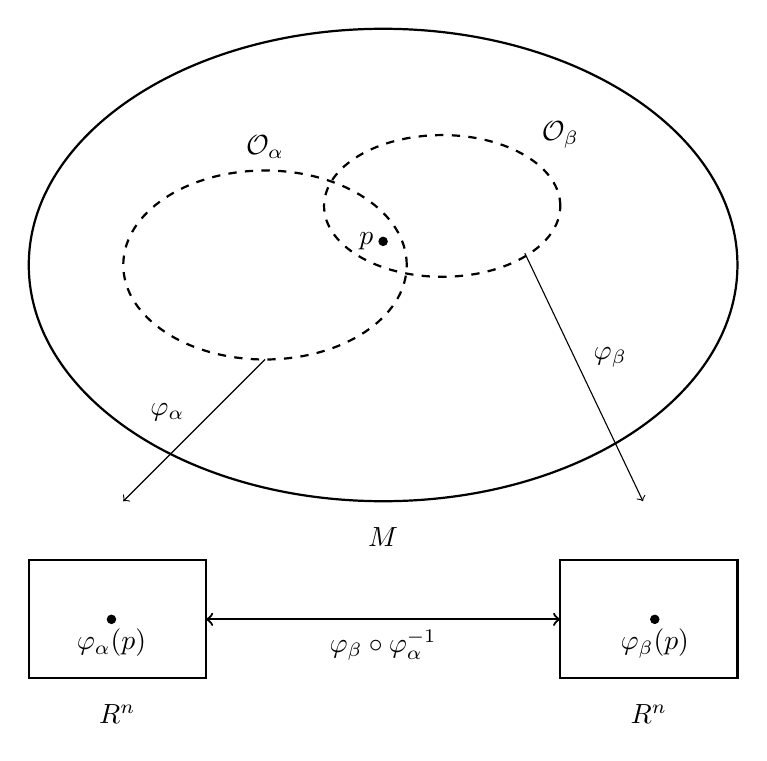
\begin{tikzpicture}[scale=1.5]

    % Define the manifold M
    \draw[thick] (0,0) ellipse (3 and 2);
    \node at (0,-2.3) {$M$}; % Label for M

    % Define open sets O_alpha and O_beta
    \draw[thick, dashed] (-1,0) ellipse (1.2 and 0.8);
    \node at (-1,1) {$\mathcal{O}_\alpha$};
    
    \draw[thick, dashed] (0.5,0.5) ellipse (1 and 0.6);
    \node at (1.5,1.1) {$\mathcal{O}_\beta$};



    % Define arrows to Euclidean spaces
    \draw[->] (-1,-0.8) -- (-2.2,-2) node[midway, above left] {$\varphi_\alpha$};
    \draw[->] (1.2,0.1) -- (2.2,-2) node[midway, above right] {$\varphi_\beta$};

    % Define Euclidean spaces
    \draw[thick] (-3,-2.5) rectangle (-1.5,-3.5);
    \node at (-2.25,-3.8) {$\mathbb{R}^n$};

    \draw[thick] (3,-2.5) rectangle (1.5,-3.5);
    \node at (2.25,-3.8) {$\mathbb{R}^n$};

    % Transition map between charts
    \draw[<->, thick] (-1.5,-3) -- (1.5,-3) node[midway, below] {$\varphi_\beta \circ \varphi_\alpha^{-1}$};

    % Points in the manifold and Euclidean space
    \filldraw (0,0.2) circle (1pt) node[left] {$p$};
    %\filldraw (1.5,0.1) circle (1pt) node[right] {$p$};

    \filldraw (-2.3,-3) circle (1pt) node[below] {$\varphi_\alpha(p)$};
    \filldraw (2.3,-3) circle (1pt) node[below] {$\varphi_\beta(p)$};

\end{tikzpicture}
\end{center}

\begin{remark}
	\begin{itemize}
		\item[]
		\item We could replace smooth with finite differentiability (e.g. $k$-times differentiable).
		\item The charts define a topology on $M$: $U \subseteq M$ is open if and only if $\phi_\alpha(U \cap O_\alpha)$ is open in $\mathbb{R}^n$ for all $\alpha$. Every open subset of $M$ is itself a manifold, by restricting the charts to $U$.
	\end{itemize}
\end{remark}

The collection $\{(O_\alpha, \phi_\alpha)\}$ is called an \emph{atlas}\index{atlas}. Two atlases are \emph{compatible}\index{compatible atlases} if their union is an atlas.

An atlas $A$ is \emph{maximal}\index{maximal atlas} if there exists no atlas $B$ which is compatible with $A$, and strictly larger than $A$. Every atlas is contained in a maximal atlas (by taking the union of all compatible atlases). Hence we can assume without loss of generality that we work with a maximal atlas.

\begin{exbox}
	\begin{enumerate}
		\item If $U \subseteq \mathbb{R}^n$ is open, we can take $O = U$, and $\phi : U \to \mathbb{R}^n$ to be the identity on $U$. Then $\{(O, \phi)\}$ is an atlas.
		\item Take $S^1$. If $p \in S^1 \setminus \{(-1, 0)\} = O_1$, there is a unique $\theta_1 \in (-\pi, \pi)$ such that
			\[
			p = (\cos \theta_1, \sin \theta_1).
			\]
			If $p \in S^1 \setminus \{(1, 0)\} = O_2$, there is a unique $\theta_2 \in (0, 2\pi)$ such that
			\[
			p = (\cos \theta_2, \sin \theta_2).
			\]
			These maps from $(-\pi, \pi)$ and $(0, 2\pi)$ to $O_1, O_2$ give $\phi_1^{-1}, \phi_2^{-1}$ respectively. Note that $\phi_1(O_1 \cap O_2) = (-\pi, 0) \cup (0, \pi)$, and the transition function is
			\[
			\phi_2 \circ \phi_1^{-1} (\theta) = 
			\begin{cases}
				\theta & \theta \in (0, \pi), \\
				\theta + 2 \pi & \theta \in (-\pi, 0).
			\end{cases}
			\]
			This is smooth where defined, and similarly for $\phi_2 \circ \phi_1^{-1}$. Hence $S^1$ is a manifold.
		\item More generally, we can consider $S^n$, and can define charts by stereographic projections. If $\{\mathbf{E}_1, \ldots, \mathbf{E}_{n+1}\}$ is the standard basis for $\mathbb{R}^{n+1}$, and $\{\mathbf{e}_1, \ldots, \mathbf{e}_n\}$ is the standard basis for $\mathbb{R}^n$, write
			\[
			\mathbf{P} = P^1 \mathbf{E}_1 + \cdots + P^{n+1} \mathbf{E}_{n+1}.
			\]
			Set $O_1 = S^n \setminus \{\mathbf{E}_{n+1}\}$, and write
			\[
			\phi_1(\mathbf{P}) = \frac{1}{1 - P^{n+1}}(P^1 \mathbf{e}_1 + \cdots + P^n \mathbf{e}_n).
			\]
			In a similar way we may define $O_2, \phi_2$, for $-\mathbf{E}_{n+1}$. The transition map is then
			\[
			\phi_2 \circ \phi_1^{-1}(\mathbf{x}) = \frac{\mathbf{x}}{|\mathbf{x}|^2},
			\]
			which is smooth on $\mathbb{R}^n \setminus \{0\} = \phi_1 (O_1 \cap O_2)$.
	\end{enumerate}
\end{exbox}

% lecture 2

``Nice'' surfaces in $\mathbb{R}^n$ are manifolds with no cusps, cornered or self-intersections, for example $S^n \subseteq \mathbb{R}^{n+1}$.

\subsection{Smooth Functions on Manifolds}%
\label{sub:smooth_fn}

Suppose $M, N$ are manifolds of dimension $n, n'$ respectively. Let $f : M \to N$.

Then let $p \in M$, and pick charts $(O_\alpha, \phi_\alpha)$ for $M$, and $(O_\beta', \phi_\beta')$ for $N$, with $p \in O_\alpha$ and $f(p) \in O_\beta$. Then,
\[
\phi_\beta' \circ f \circ \phi_\alpha^{-1}
\]
maps a neighbourhood of $\phi_\alpha(p)$ in $U_\alpha \subseteq \mathbb{R}^n$, to $U_\beta' \in \mathbb{R}^{n'}$. If this function is smooth for all possible choices of this chart, we say that $f : M \to N$ is smooth.

\begin{center}
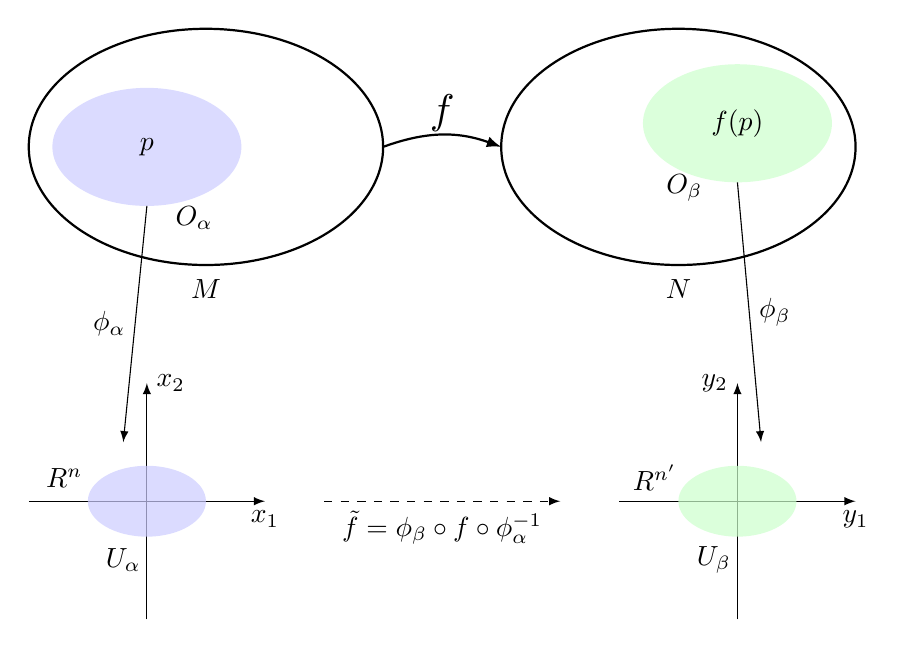
\begin{tikzpicture}[scale=1.5,>=latex]

    % Draw manifold M (as an ellipse) and mark the chart O_alpha
    \draw[thick] (-2,0) ellipse (1.5 and 1);  % Manifold M
    \node at (-2,-1.2) {$M$};  % Label M

    % Draw chart O_alpha as a shaded region on M
    \fill[blue!20,opacity=0.7] (-2.5,0) ellipse (0.8 and 0.5);
    \node at (-2.1,-0.6) {$O_\alpha$};
    \node at (-2.5,0) {$p$};  % Label point p

    % Draw manifold N (as an ellipse) and mark the chart O_beta
    \draw[thick] (2,0) ellipse (1.5 and 1);  % Manifold N
    \node at (2,-1.2) {$N$};  % Label N

    % Draw chart O_beta as a shaded region on N
    \fill[green!20,opacity=0.7] (2.5,0.2) ellipse (0.8 and 0.5);
    \node at (2.05,-0.35) {$O_\beta$};
    \node at (2.5,0.2) {$f(p)$};  % Label point f(p)

    % Draw smooth map f from M to N
    \draw[->, thick] (-0.5,0) to [out=20,in=160] (0.5,0) node[midway,above] {$f$};

    % Add Euclidean spaces R^n and R^{n'}
    %\node at (-2,-2.5) (Rn) {$\mathbb{R}^n$};
    %\node at (2,-2.5) (Rnp) {$\mathbb{R}^{n'}$};

    % Map from O_alpha to R^n
    %\draw[->] (-2.5,-0.6) -- (-2,-2) node[midway,left] {$\phi_\alpha$};

    % Map from O_beta to R^{n'}
    %\draw[->] (2.5,0.5) -- (2,-2) node[midway,right] {$\phi_\beta$};

    % Dashed arrow for the map between R^n and R^{n'}
    %\draw[->, dashed] (Rn) -- (Rnp) node[midway,below] {$\tilde{f} = \phi_\beta \circ f \circ \phi_\alpha^{-1}$};

 % Add Euclidean spaces R^n and R^{n'} as axes
    % R^n axes
    \draw[->] (-3.5,-3) -- (-1.5,-3) node[anchor=north] {$x_1$};
    \draw[->] (-2.5,-4) -- (-2.5,-2) node[anchor=west] {$x_2$};
    \node at (-3.2,-2.8) {$\mathbb{R}^n$};

    % R^{n'} axes
    \draw[->] (1.5,-3) -- (3.5,-3) node[anchor=north] {$y_1$};
    \draw[->] (2.5,-4) -- (2.5,-2) node[anchor=east] {$y_2$};
    \node at (1.8,-2.8) {$\mathbb{R}^{n'}$};

    % Map from O_alpha to R^n
    \draw[->] (-2.5,-0.5) -- (-2.7,-2.5) node[midway,left] {$\phi_\alpha$};

    % Map from O_beta to R^{n'}
    \draw[->] (2.5,-0.3) -- (2.7,-2.5) node[midway,right] {$\phi_\beta$};

    % Dashed arrow for the map between R^n and R^{n'}
    \draw[->, dashed] (-1,-3) -- (1,-3) node[midway,below] {$\tilde{f} = \phi_\beta \circ f \circ \phi_\alpha^{-1}$};

    % Draw open sets U_alpha in R^n and U_beta in R^{n'}
    \fill[blue!20,opacity=0.7] (-2.5,-3) ellipse (0.5 and 0.3);
    \node at (-2.7,-3.5) {$U_\alpha$};

    \fill[green!20,opacity=0.7] (2.5,-3) ellipse (0.5 and 0.3);
    \node at (2.3,-3.5) {$U_\beta$};

\end{tikzpicture}
\end{center}

\begin{remark}
	\begin{itemize}
		\item[]
		\item A smooth map $\psi : M \to N$ which has a smooth inverse is called a \emph{diffeomorphism}\index{diffeomorphism}.
		\item If $N = \mathbb{R}$ or $\mathbb{C}$, we sometimes call $f$ a \emph{scalar field}\index{scalar field}.
		\item If $M = I \subseteq \mathbb{R}$, an open interval, then $f : I \to N$ is a \emph{smooth curve} in $N$.
		\item If $f$ is smooth in one atlas, then it is smooth in all compatible atlases.
	\end{itemize}
\end{remark}

\begin{exbox}
	\begin{enumerate}
		\item Recall $S^1$. Let $f(x, y) = x$, $f : S^1 \to \mathbb{R}$. Using our previous charts,
			\begin{align*}
				f \circ \phi_1^{-1} : (-\pi, \pi) &\to \mathbb{R} \\
				\theta_1 \mapsto \cos \theta_1.
			\end{align*}
			Similarly,
			\begin{align*}
				f \circ \phi_2^{-1} : (0, 2\pi) &\to \mathbb{R} \\
				\theta_2 \mapsto \cos \theta_2.
			\end{align*}
			Hence $f$ is smooth.
		\item If $(O, \phi)$ is a coordinate chart on $M$, write
			\[
			\phi(p) = (x^1(p), x^2(p), \ldots, x^n(p)),
			\]
			for $p \in O$. Then $x^i(p)$ defines a map from $O$ to $\mathbb{R}$. This is smooth for each $i = 1, \ldots, n$. If $(O', \phi')$ is another overlapping coordinate chart, then $x^i \circ (\phi')^{-1}$ is the $i$'th component of $\phi \circ (\phi')^{-1}$, hence smooth.
		\item We can define a smooth function chart-by-chart. For simplicity, let $N = \mathbb{R}$, and let $\{(O_\alpha, \phi_\alpha)\}$ be an atlas on $M$. Define smooth functions
			\[
			F_\alpha : U_\alpha \to \mathbb{R},
			\]
			and suppose that $F_\alpha \circ \phi_\alpha = F_\beta \circ \phi_\beta$ on $O_\alpha \cap O_\beta$, for all $\alpha, \beta$.

			Then for $p \in M$, we can define
			\[
			f(p) = F_\alpha \circ \phi_\alpha(p),
			\]
			for any chart $(O_\alpha, \phi_\alpha)$ with $p \in O_\alpha$. Now $f$ is smooth, as
			\[
			f \circ \phi_p^{-1} = F_\alpha \circ \phi_\alpha \circ \phi_\beta^{-1}.
			\]
			In practice, we often don't distinguish between $f$ and its coordinate chart representations $F_\alpha$.
	\end{enumerate}	
\end{exbox}

\subsection{Curves and Vectors}%
\label{sub:cav}

For a surface in $\mathbb{R}^3$, we have a notion of the `tangent space' at a point $p$, which consists of all vectors tangent to the surface at that point.

The tangent spaces are vector spaces (copies of $\mathbb{R}^2$). Different points have different tangent spaces.

In order to define the tangent space for a manifold, we first consider tangent vectors of a curve.

Recall that $\lambda : I \to M$ a smooth map, is a smooth curve in $M$.

If $\lambda(t)$ is a smooth curve in $\mathbb{R}^n$, and $f : \mathbb{R}^n \to \mathbb{R}$ is a smooth function, the chain rule gives
\[
	\frac{\diff}{\diff t} [f(\lambda(t))] = X(t) \cdot \nabla f(\lambda(t)),
\]
where $X(t) = \diff \lambda / \diff t (t)$ is the tangent vector to $\lambda$ at $t$.

\begin{definition}
	Let $\lambda : I \to M$ be a smooth curve with $\lambda(0) = p$. The \emph{tangent vector}\index{tangent vector} to $\lambda$ at $p$ is the linear map $X_p$ from the space of smooth functions $f : M \to \mathbb{R}$, given by
	\[
	X_p(f) = \frac{\diff}{\diff t} f(\lambda(t)) \biggr|_{t = 0}.
	\]
\end{definition}

We observe that:
\begin{enumerate}[(i)]
	\item $X_p$ is linear: $X_p(f + a g) = X_p(f) + a X_p (g)$, for $f, g$ smooth, and $a \in \mathbb{R}$.
	\item $X_p$ satisfies the Leibniz rule:
		\[
		X_p(fg) = X_p(f) g(p) + f(p) X_p(g).
		\]
\end{enumerate}

If $(O, \phi)$ is a chart and $p \in O$, write
\[
\phi(p) = (x^1(p), \ldots, x^n(p)).
\]
Let $F = f \circ \phi^{-1}$, and $x^i(t) = x^i(\lambda(t))$. Now $F : \mathbb{R}^n \to \mathbb{R}$, and $x : \mathbb{R} \to \mathbb{R}^n$. Then,
\[
f \circ \lambda(t) = f \circ \phi^{-1} \circ \phi \circ \lambda(t) = F \circ x(t),
\]
and by applying the regular chain rule for functions $\mathbb{R}^m \to \mathbb{R}^n$,
\[
\frac{\diff}{\diff t} f(\lambda(t)) \biggr|_{t = 0} = \frac{\partial F}{\partial x^\mu} (x) \cdot \frac{\diff x^\mu}{\diff t} \biggr|_{t = 0}.
\]

% lecture 3

\begin{proposition}
	The set of tangent vectors to curves at $p$ forms a vector space, $T_pM$, of dimension $n = \dim M$. We call $T_p M$ the \emph{tangent space}\index{tangent space} to $M$ at $p$.
\end{proposition}

\begin{proofbox}
	Given $X_p, Y_p$ tangent vectors, we need to show that $\alpha X_p + \beta Y_p$ is a tangent vector for $\alpha, \beta \in \mathbb{R}$.

	Let $\lambda, \kappa$ be smooth curves with $\lambda(0) = \kappa(0) = p$, and whose tangent vectors at $p$ are $X_p, Y_p$, respectively.

	Let $(O, \phi)$ be a chart with $p \in O$ and $\phi(p) = 0$, and define
	\[
	\gamma(t) = \phi^{-1}( \alpha \phi(\lambda (t)) + \beta \phi (\kappa (t)) ).
	\]
	This exists, as this is just the sum of elements in $\mathbb{R}^n$.

	Now $\gamma(0) = \phi^{-1}(0) = p$. If $Z_p$ is the tangent to $v$ at $p$, then
	\begin{align*}
		Z_p(f) &= \frac{\diff}{\diff t} f(v(t)) \biggr|_{t = 0} = \frac{\partial F}{\partial x^\mu} \biggr|_{0} \frac{\diff}{\diff t} [\alpha x^\mu (\lambda(t)) + \beta x^\mu(\kappa(t)) ] \biggr|_{t = 0} \\
		       &= \alpha \frac{\partial F}{\partial x^\mu} \biggr|_0 \frac{\diff}{\diff t} x^\mu(\lambda(t)) \biggr|_{t = 0} + \beta \frac{\partial F}{\partial x^\mu} \biggr|_0 \frac{\diff}{\diff t} x^\mu(\kappa(t)) \biggr|_{t =0} \\
		       &= \alpha X_p(f) + \beta Y_p(f).
	\end{align*}
	Thus $T_p M$ is a vector space.

	To see that $T_p M$ is $n$-dimensional, consider the curves
	\[
		\lambda_\mu(t) = \phi^{-1} \underbrace{(0, \ldots, 0, t, 0, \ldots, 0).}_{\mu\text{'th component}}
	\]
	We denote the tangent vector to $\lambda_\mu$ at $p$ by $(\partial / \partial x^\mu)_p$. To see why, note that
	\[
	\left(\frac{\partial}{\partial x^\mu} \right)_p f = \frac{\partial F}{\partial x^\mu} \biggr|_{\phi(p) = 0}.
	\]

	These vectors are linearly independent. Otherwise there exists $\alpha^\mu$ not all zero such that
	\[
	\alpha^\mu \left( \frac{\partial}{\partial x^\mu} \right)_p = 0 \implies \alpha^\mu \frac{\partial F}{\partial x^\mu} \biggr|_0 = 0,
	\]
	for all $F$. Setting $F = x^\nu$ gives $\alpha^\nu = 0$.

	Further, these vectors form a basis for $T_p M$, since if $\lambda$ is any curve with tangent $X_p$ at $p$, then
	\[
	X_p(f) = \frac{\partial F}{\partial x^\mu} \biggr|_0 \frac{\diff}{\diff t} x^\mu(\lambda(t)) \biggr|_{t = 0} = X^\mu \left( \frac{\partial}{\partial x^\mu} \right) f.
	\]
	Here, we set
	\[
	X^\mu = \frac{\diff}{\diff t} x^\mu(\lambda(t)) \biggr|_{t = 0}.
	\]
	These are the components of $X_p$ with respect to the basis.
\end{proofbox}

\begin{center}
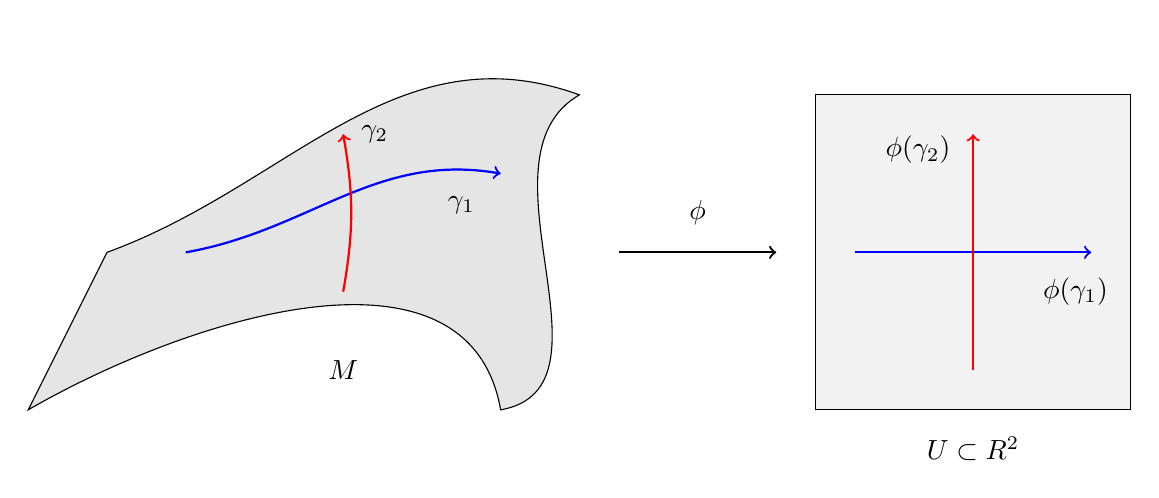
\begin{tikzpicture}

% Manifold M (2D surface, wavy shape)
\draw[fill=gray!20] (0,0) to[out=20,in=160] (6,2) to[out=-150,in=10] (5,-2) to[out=100, in=30] (-1, -2) -- cycle;
\node at (3, -1.5) {$M$};

% Horizontal path on M (blue)
\draw[thick, blue, ->] (1,0) to[out=10,in=170] (5,1);
\node at (4.5, 0.6) {$\gamma_1$};

% Vertical path on M (red)
\draw[thick, red, ->] (3,-0.5) to[out=80,in=-80] (3,1.5);
\node at (3.4, 1.5) {$\gamma_2$};

% Projection map phi
\draw[->, thick] (6.5,0) -- (8.5,0);
\node at (7.5, 0.5) {$\phi$};

% Open set U in R^2 (rectangle)
\draw[fill=gray!10] (9, 2) rectangle (13, -2);
\node at (11, -2.5) {$U \subset \mathbb{R}^2$};

% Projection of horizontal path in U
\draw[thick, blue, ->] (9.5,0) -- (12.5,0);
\node at (12.3, -0.5) {$\phi(\gamma_1)$};

% Projection of vertical path in U
\draw[thick, red, ->] (11,-1.5) -- (11,1.5);
\node at (10.3, 1.3) {$\phi(\gamma_2)$};

% Axes in U (x and y)
%\draw[->] (9,-4.5) -- (9,-0.5) node[anchor=south east] {$y$};
%\draw[->] (9,-4.5) -- (13,-4.5) node[anchor=north west] {$x$};

\end{tikzpicture}
\end{center}

Notice that the basis $\{(\partial / \partial x^\mu)_p\}$ depends on the coordinate chart $\phi$. Suppose we choose another chart $(O', \phi')$, again centred at $p$. Write $\phi' = (x'^1, \ldots, x'^n)$.

Then if $F\ = f \circ (\phi')^{-1}$, then
\begin{align*}
	F(x) & = f \circ \phi^{-1}(x) = f \circ (\phi')^{-1} \circ \phi' \circ \phi^{-1}(x)  \\
	     &= F'(x'(x)).
\end{align*}
Therefore,
\[
	\left( \frac{\partial}{\partial x^\mu} \right)_p f = \frac{\partial F}{\partial x^\mu} \biggr|_{\phi(p)} = \left( \frac{\partial x'^\nu}{ \partial x^\mu} \right)_{\phi(p)} \left( \frac{\partial F'}{\partial x'^\nu} \right)_{\phi'(p)} = \left( \frac{\partial x'^\nu}{ \partial x^\mu} \right)_{\phi(p)} \cdot \left( \frac{\partial}{\partial x'^\nu} \right)_p f.
\]
We deduce that
\[
\left( \frac{\partial}{\partial x^\mu} \right)_p = \left( \frac{\partial x'^\nu}{\partial x^\mu}\right)_{\phi(p)} \left( \frac{\partial}{\partial x'^\nu} \right)_p.
\]
So let $X^\mu$ be the components of $X_p$ with respect to $\{(\partial / \partial x^\mu)_p\}$, and $X'^\mu$ be the components with respect to $\{(\partial / \partial x'^\mu)_p\}$. So,
\begin{align*}
	X_p &= X^\mu \left( \frac{\partial}{\partial x^\mu} \right)_p = X'^\mu \left( \frac{\partial}{\partial x'^\mu} \right)_p \\
	    &= X^\mu \left( \frac{\partial x'^\sigma}{\partial x^\mu} \right)_{\phi(p)} \left( \frac{\partial}{\partial x'^\sigma} \right)_p.
\end{align*}
Therefore,
\[
X'^\mu = \left( \frac{\partial x'^\mu}{\partial x^\nu} \right)_{\phi(p)} X^\nu.
\]
We do not have to choose a coordinate basis such as $\{(\partial/\partial x^\mu)_p\}$. With respect to a general basis $\{e_\mu\}$ for $T_p M$, we write $X_p = X^\mu e_\mu$, for $X^\mu \in \mathbb{R}$ the components.

We always use summation conventions: we always contract one upstairs and one downstairs index.

\subsection{Covectors}%
\label{sub:cov}

Recall that if $V$ is a vector space over $\mathbb{R}$, the \emph{dual space}\index{dual space} $V^\ast$ is the space of linear maps from $V$ to $\mathbb{R}$. If $V$ is $n$-dimensional, then so is $V^\ast$.

Given a basis $\{e_\mu\}$ for $V$, we define the \emph{dual basis}\index{dual basis} $\{f^\mu\}$ for $V^\ast$ by requiring that
\[
f^\mu(e_\nu) = \delta\indices{^{\mu}_{\nu}}.
\]
If $V$ is finite dimensional, then $V^{\ast\ast} = (V^\ast)^\ast$ is isomorphic to $V$: to an element $x$ of $V$, we assign a linear map $\Lambda_x : V^\ast \to \mathbb{R}$ by
\[
\Lambda_x(\omega) = \omega(x).
\]
\begin{definition}
	The dual space of $T_pM$ is denoted $T^\ast_p M$, and is called the \emph{cotangent space}\index{cotangent space} to $M$ at $p$.

	An element of this space is a covector at $p$. If $\{e_\mu\}$ is a basis for $T_p M$ and $\{f^\mu\}$ the dual basis for $T^\ast_p M$, then we can expand a covector $\eta$ as
	\[
	\eta = \eta_\mu f^\mu,
	\]
	for $\eta_\mu \in \mathbb{R}$ the components of $\eta$.
\end{definition}

% lecture 4

Note that:
\begin{itemize}
	\item $\eta(e_\nu) = \eta_\mu f^\mu (e_\nu) = \eta_\mu \delta\indices{^{\mu}_{\nu}} = \eta_\nu$.
	\item $\eta(X) = \eta(X^\mu e_\mu) = X^\mu \eta(e_\mu) = X^\mu \eta_\mu$.
\end{itemize}

\begin{definition}
	If $f : M \to \mathbb{R}$ is a smooth function, define $(\diff f)_p \in T^\ast_p M$, the \emph{differential}\index{differential} of $f$ at $p$, by
	\[
		(\diff f)_p (X) = X(f),
	\]
	for any $X \in T_p M$. $(\diff f)_p$ is sometimes also called the \emph{gradient}\index{gradient} of $f$ at $p$.
\end{definition}

If $f$ is a constant, then $X(f) = 0 \implies (\diff f)_p = 0$.

If $(O, \phi)$ is a coordinate chart with $p \in O$ and $\phi = (x^1, \ldots, x^n)$, then we can set $f = x^\mu$ to find $(\diff x^\mu)_p$. Now,
\[
	(\diff x^\mu)_p \left( \frac{\partial}{\partial x^\nu} \right)_p = \left( \frac{\partial x^\mu}{\partial x^\nu} \right)_{\phi(p)} = \delta\indices{^{\mu}_{\nu}}.
\]
Hence, $\{(\diff x^\mu)_p\}$ is the dual basis to $\{(\partial/\partial x^\mu)_p\}$. In this basis, we can compute
\[
	[(\diff f)_p]_\mu = (\diff f)_p \left( \frac{\partial}{\partial x^\mu} \right)_p = \left( \frac{\partial}{\partial x^\mu} \right)_p f = \left( \frac{\partial F}{\partial x^\mu} \right)_{\phi(p)},
\]
justifying the language of the `gradient'.

It can be shown that if $(O', \phi')$ is another chart with $p \in O'$, then
\[
	(\diff x^\mu)_p = \left( \frac{\partial x^\mu}{\partial x'^\nu} \right)_{\phi'(p)} (\diff x'^\nu)_p,
\]
where $x(x') = \phi \circ \phi'^{-1}$, and hence if $\eta_\mu$, $\eta'_\mu$ are components with respect to these bases, then
\[
\eta_\mu' = \left(\frac{\partial x^\nu}{\partial x'^\mu} \right)_{\phi'(p)} \eta_\nu.
\]

\subsection{The (Co)tangent bundle}%
\label{sub:tb}

We can glue together the tangent spaces $T_pM$ as $p$ varies to get a new $2n$ dimensional manifold, $TM$, the \emph{tangent bundle}\index{tangent bundle}. We let
\[
	TM = \bigcup_{p \in M} \{p\} \times T_pM,
\]
the set of ordered pairs $(p, X)$, with $p \in M$, $X \in T_pM$. If $\{(O_\alpha, \phi_\alpha)\}$ is an atlas on $M$, we obtain an atlas for $TM$ by setting
\[
	\tilde O_\alpha = \bigcup_{p \in O_\alpha} \{p\} \times T_p M,
\]
and
\[
\tilde \phi_\alpha((p, X)) = (\phi_\alpha(p), X^\mu) \in U_\alpha \times \mathbb{R}^{n} = \tilde U_\alpha,
\]
where $X^\mu$ are the components of $X$ with respect to the coordinate basis of $\phi_\alpha$.

It can be shown that if $(O, \phi)$ and $(O', \phi')$ are two charts on $M$, on $\tilde U \cap \tilde U'$, if we write $\phi' \circ \phi^{-1}(x) = x'(x)$, then
\[
\tilde \phi' \circ \tilde \phi^{-1}(x, X^\mu) = \left( x'(x), \frac{\partial x'^\mu}{\partial x^\nu} X^\nu \right).
\]
This lets us deduce that $TM$ is a manifold.

A similar construction permits us to define the \emph{cotangent bundle}\index{cotangent bundle}
\[
	T^\ast M = \bigcup_{p \in M} \{p\} \times T_p^\ast M.
\]
The map $\pi : TM \to M$ which takes $(p, X) \mapsto p$ is smooth (show this!)

\subsection{Abstract Index Notation}%
\label{sub:ain}

We have used Greek letters $\mu, \nu$ to label components of vectors (or covectors) with respect to the bases $\{e_\mu\}$. Equations involving these quantities refer to the specific basis, for example if we write $X^\mu = \delta^\mu$, this says $X$ only has one non-zero component \emph{in the current basis}, which will not be true in other bases.

However, we know that some equations hold in all bases, e.g.
\[
\eta(X) = X^\mu \eta_\mu.
\]
To capture this, we can use \emph{abstract index notation}\index{abstract index notation}. We denote a vector by $X^a$, where the latin index $a$ does not denote a component, rather it tells us that $X^a$ is a vector. Similarly we denote a covector $\eta$ by $\eta_a$.

If an equation is true in all bases, then we can replace Greek indices by latin indices:
\[
\eta(X) = X^a \eta_a = \eta_a X^a,
\]
or
\[
X(f) = X^a (\diff f)_a.
\]
An equation in abstract index notation can always be turned into an equation for components, by picking a basis and changing $a \to \mu$, $b \to \nu$.

\subsection{Tensors}%
\label{sub:tens}

In Newtonian physics, we know that some quantities are described by higher rank orders, e.g. the inertia tensor or the metric.

\begin{definition}
	A \emph{tensor}\index{tensor} of type $(r, s)$ is a multilinear map
	\[
		T : (T^\ast_p M)^r \times (T_p M)^s \to \mathbb{R}.
	\]
\end{definition}

\begin{exbox}
	\begin{enumerate}
		\item A tensor of type $(0, 1)$ is a linear map $T_p M \to \mathbb{R}$, i.e. just a covector.
		\item A tensor of type $(1, 0)$ is a linear map $T^\ast p M \to \mathbb{R}$, i.e. an element of $(T^\ast p M)^\ast \cong T_p M$, a vector.
		\item We can define a $(1, 1)$ tensor $\delta$ by
			\[
			\delta(\omega, X) = \omega(X),
			\]
		where $\omega \in T_p^\ast M$, $X \in T_p M$.
	\end{enumerate}
\end{exbox}

If $\{e_\mu\}$ is a basis for $T_p M$ and $\{f^\mu\}$ its dual basis, then the components of an $(r, s)$ tensor $T$ are
\[
T\indices{^{\mu_1 \cdots \mu_r}_{\nu_1 \cdots \nu_s}} = T(f^\mu_1, \ldots, f^{\mu_r}, e_{\nu_1}, \ldots, e_{\nu_s}).
\]
In abstract index notation, we denote $T$ by $T\indices{^{a_1 \cdots a_r}_{b_1 \cdots b_s}}$. Tensors at $p$ form a vector space over $\mathbb{R}$ of dimension $n^{r + s}$.

\begin{exbox}
	\begin{enumerate}
		\item Consider $\delta$ above. Then,
			\[
			\delta\indices{^{\mu}_{\nu}} = \delta(f^\mu, e_\nu) = f^\mu(e_\nu) =
			\begin{cases}
				1 & \mu = \nu,\\
				0 & \mu \neq \nu.
			\end{cases}
			\]
			We can write $\delta$ as $\delta\indices{^{a}_{b}}$ in AIN.
		\item Consider a $(2, 1)$ tensor $T$, and let $\omega, \eta \in T_p^\ast M$, $X \in T_p M$. Then,
			\begin{align*}
				T(\omega, \eta, X) &= T(\omega_\mu f^\mu, \eta_\nu f^\nu, X^\sigma e_\sigma) \\
						   &= \omega_\mu \eta_\nu X^\sigma T(f^\mu, f^\nu, e_\sigma) \\
						   &= \omega_\mu \eta_\nu X^\sigma T\indices{^{\mu\nu}_{\sigma}}.
			\end{align*}
			In AIN,
			\[
			T(\omega, \nu, X) = \omega_a \eta_b X^c T\indices{^{ab}_{c}}.
			\]
			This can be generalized to higher ranks.
	\end{enumerate}
	
\end{exbox}

% lecture 5

\subsection{Change of Bases}%
\label{sub:cob}

We have already seen how the components of $X$ or $\eta$ with respect to a coordinate basis ($X^\mu, \eta_\nu$ respectively) change under a change of coordinates.

But we do not only have to consider coordinate bases.

Suppose $\{e_\mu\}$ and $\{e'_\mu\}$ are two bases for $T_pM$ with dual bases $\{f^\mu\}$ and $\{f'^\mu\}$.

As these are bases, we can expand
\[
f'^\mu = A\indices{^{\mu}_{\nu}} f^\nu, \qquad e'_\mu = B\indices{^{\nu}_{\mu}} e_\nu,
\]
for some $A\indices{^{\mu}_{\nu}}, B\indices{^{\mu}_{\nu}} \in \mathbb{R}$. But,
\begin{align*}
	\delta\indices{^{\mu}_{\nu}} &= f'^\mu (e'_\nu) = A\indices{^{\mu}_{\tau}} f^\tau ( B\indices{^{\sigma}_{\nu}} e_\sigma) \\
				     &= A\indices{^{\mu}_{\tau}} B\indices{^{\sigma}_{\nu}} f^\tau(e_\sigma) = A\indices{^{\mu}_{\tau}} B\indices{^{\sigma}_{\nu}} \delta\indices{^{\tau}_{\sigma}} \\
				     &= A\indices{^{\mu}_{\sigma}} B\indices{^{\sigma}_{\nu}}.
\end{align*}
Therefore, looking at these as matrices,
\[
B\indices{^{\mu}_{\nu}} = (A^{-1})\indices{^{\mu}_{\nu}}.
\]
If
\[
e_\mu = \left( \frac{\partial}{\partial x^\mu} \right)_p, \qquad e'_\mu = \left( \frac{\partial}{\partial x'^\mu} \right)_p,
\]
then we have already seen
\[
A\indices{^{\mu}_{\nu}} = \left( \frac{\partial x'^\mu}{\partial x^\nu} \right)_{\phi(p)}, \qquad B\indices{^{\mu}_{\nu}} = \left( \frac{\partial x^\mu}{\partial x'^\nu} \right)_{\phi(p)},
\]
which indeed satisfies $A\indices{^{\mu}_{\sigma}}B\indices{^{\sigma}_{\nu}} = \delta\indices{^{\mu}_{\nu}}$, by the chain rule.

A chance of bases induces a transformation of tensor components, for example if $T$ is a $(1, 1)$-tensor, then
\begin{align*}
	T\indices{^{\mu}_{\nu}} &= T(f^\mu, e_\nu) \\
	{T'}\indices{^{\mu}_{\nu}} &= T(f'^\mu, e'_\nu) = T(A\indices{^{\mu}_{\sigma}} f^\sigma, (A^{-1})\indices{^{\tau}_{\nu}} e_\tau ) \\
				 &= A\indices{^{\mu}_{\sigma}} (A^{-1})\indices{^{\tau}_{\nu}} T(f^\sigma, e_\tau) \\
				 &= A\indices{^{\mu}_{\sigma}} (A^{-1})\indices{^{\tau}_{\nu}} T\indices{^{\sigma}_{\tau}}.
\end{align*}


\subsection{Tensor Operations}%
\label{sub:top}

Given an $(r, s)$-tensor, we can form a $(r - 1, s-1)$-tensor by \emph{contraction}\index{contraction}.

For simplicity, assume $T$ is a $(2, 2)$-tensor. Define a $(1, 1)$-tensor $S$ by
\[
S(\omega, X) = T(\omega, f^\mu, X, e_\mu).
\]
To see that this is independent of the choice of basis, note
\begin{align*}
	T(\omega, f'^\mu, X, e'_\mu) &= T(\omega, A\indices{^{\mu}_{\sigma}} f^\sigma, X, (A^{-1})\indices{^{\tau}_{\mu}} e_\tau ) = A\indices{^{\mu}_{\sigma}} (A^{-1})\indices{^{\tau}_{\mu}} T(\omega, f^\sigma, X, e_\tau) \\
				     &= \delta\indices{^{\tau}_{\sigma}} T(\omega, f^\sigma, X, e_\tau) = T(\omega, f^\tau, X, e_\tau) = S(\omega, X).
\end{align*}
So this does not depend on the choice of basis. $S$ and $T$ have components related by
\[
S\indices{^{\mu}_{\nu}} = T\indices{^{\mu\sigma}_{\nu\sigma}}.
\]
In any basis in AIN we write
\[
S\indices{^{a}_{b}} = T\indices{^{ac}_{bc}}.
\]
We can generalise to contract any upstairs index with any downstairs index in a general $(r, s)$-tensor.

Another way to make new tensors from old tensors is to form the \emph{tensor product}\index{tensor product}. If $S$ is a $(p, q)$-tensor and $T$ is a $(r, s)$-tensor, then $S \otimes T$ is an $(p + r, q + s)$-tensor:
\begin{align*}
	S \otimes &T(\omega^1, \ldots, \omega^p, \eta^1, \ldots, \eta^r, X_1, \ldots, X_q, Y_1, \ldots, Y_s) \\
		  &= S(\omega^1, \ldots, \omega^p, X_1, \ldots, X_q) T(\eta^1, \ldots, \eta^r, Y_1, \ldots, Y_s).
\end{align*}
This is independent of basis. In AIN,
\[
	(S \otimes T)\indices{^{a_1\ldots a_p b_1 \ldots b_r}_{c_1 \ldots c_q d_1 \ldots, d_s}} = S\indices{^{a_1 \ldots a_r}_{ c_1 \ldots c_q}} T\indices{^{b_1 \ldots b_r}_{d_1 \ldots b_r}}.
\]
We can show that for any $(1, 1)$-tensor $T$, in any basis we have
\[
T = T\indices{^{\mu}_{\nu}} e_\mu \otimes f^\nu.
\]
The final tensor operations we require are \emph{(anti)symmetrization}\index{symmetrization}\index{antisymmetrization}. If $T$ is a $(0, 2)$-tensor, we can define two new tensors:
\begin{align*}
	S(X, Y) &= \frac{1}{2}(T(X, Y) + T(Y, X)), \\
	A(X, Y) &= \frac{1}{2} (T(X, Y) - T(Y, X)).
\end{align*}
In AIN,
\begin{align*}
	S_{ab} = \frac{1}{2} (T_{ab} + T_{ba}) = T_{(ab)}, \\
	A_{ab} = \frac{1}{2} (T_{ab} - T_{ba}) = T_{[ab]}.
\end{align*}
These operations can be applied to any pair of matching symmetries in a more general tensor, for example:
\[
T\indices{^{a(bc)}_{de}} = \frac{1}{2} (T\indices{^{abc}_{de}} + T\indices{^{acb}_{de}}).
\]
We can also (anti)symmetrize over more than two indices.
\begin{itemize}
	\item To symmetrize over $n$ indices, we sum over all permutations of the indices and divide by $n!$.
	\item To anti-symmetrize over $n$ indices, we sum over all permutation weighted by their sign, and then divide by $n!$.
\end{itemize}

For example,
\begin{align*}
	T^{(abc)} &= \frac{1}{3!} (T^{abc} + T^{bca} + T^{cab} + T^{acb} + T^{cba} + T^{bac}), \\
	T^{[abc]} &= \frac{1}{3!} (T^{abc} + T^{bca} + T^{cab} - T^{acb} - T^{cba} - T^{bac}).
\end{align*}
To exclude indices from (anti)symmetrization, we use vertical lines:
\[
T^{(a|b|c)} = \frac{1}{2} (T^{abc} + T^{c b a}).
\]
\subsection{Tensor Bundles}%
\label{sub:tense_buns}

The space of $(r, s)$-tensors at a point $p$ is the vector space $(T\indices{^{r}_{s}})_pM$. These can be glued together to form the bundle of $(r, s)$-tensors
\[
	T\indices{^{r}_{s}} M = \bigcup_{p \in M}\{ p\} \times (T\indices{^{r}_{s}} )_p M.
\]
If $(O, \phi)$ is a coordinate chart on $M$, set
\[
	\tilde O = \bigcup_{p \in O} \{p\} \times (T{\indices{^{r}_{s}}})_p M \subseteq T\indices{^{r}_{s}}M,
\]
and
\[
\tilde \phi(p, S_p) = (\phi(p), S\indices{^{\mu_1 \ldots \mu_r}_{\nu_1 \ldots \nu_s}} ).
\]
$T\indices{^{r}_{s}} M$ is a manifold, with a natural smooth map $\Pi : T\indices{^{r}_{s}}M \to M$ such that $\Pi(p, S_p) = p$.

A \emph{tensor field}\index{tensor field} is a smooth map $T : M \to T\indices{^{r}_{s}}M$ such that $\pi \circ T = \id$.

If $(O, \phi)$ is a coordinate chart on $M$, then
\[
\tilde \phi \circ T \circ \phi(x) = (x, T\indices{^{\mu_1 \ldots \mu_r}_{ \nu_1 \ldots \nu_s}}(x)),
\]
which is smooth provided the components $T\indices{^{\mu_1 \ldots, \mu_r}_{ \nu_1 \ldots \nu_s}}(x)$ are smooth functions of $x$.

\begin{exbox}
	If $T\indices{^{r}_{s}} M = T\indices{^{1}_{0}}M \cong TM$, the tensor field is called a \emph{vector field}\index{vector field}. In a local coordinate patch, if $X$ is a vector field, we write $X(p) = (p, X_p)$, with
	\[
	X_p = X^\mu(x) \left( \frac{\partial}{\partial x^\mu} \right)_p.
	\]
	In particular, $\partial / \partial x^\mu$ are always smooth, but only defined locally.
\end{exbox}

% lecture 6

A vector field can act on a function $f : M \to \mathbb{R}$ to give a new function $Xf$ by
\[
Xf(p) = X_p(f).
\]
In coordinates,
\[
Xf(p) = X^\mu(\phi(p)) \frac{\partial F}{\partial x^\mu} \biggr|_{\phi(p)},
\]
where $F = f \circ \phi^{-1}$.

\subsection{Integral Curves}%
\label{sub:ic}

Given a vector field $X$ on $M$, we say a curve $\lambda : I \to M$ is an \emph{integral curve}\index{integral curve} of $X$ if its tangent at every point $x$, which we denote by $\diff \lambda/ \diff t$, then
\[
\frac{\diff \lambda}{\diff t} (t) = X_{\lambda(t)}.
\]
Through each point $p$, there is a unique integral curve passing through it, unique up to extension or shift of the parameter.

To see this, pick a chart $\phi$ with $\phi = (x^1, \ldots, x^n)$, and $\phi(p) = 0$. In this chart, the equation becomes
\[
\frac{\diff x^\mu}{\diff t}(t) = X^\mu(x(t)),
\]
where $x^\mu(t) = x^\mu(\lambda(t))$. Assuming without loss of generality that $\lambda(0) = p$, we get an initial condition $x^\mu(0)= 0$.

By standard ODE theory, this equation with initial conditions has a solution which is unique up to extension.

\subsection{Commutators}%
\label{sub:com}

Suppose $X$ and $Y$ are two vector fields, and $f : M \to \mathbb{R}$ is smooth. Then $X(Y(f))$ is a smooth function, however it is not of the form $K(f)$ for some vector field $K$, since
\begin{align*}
	X(Y(fg)) &= X(f Y(g) + g Y(f)) = X(f(Y(g)) + X(g Y(f)) \\
		 &= f X(Y(g)) + g X(Y(f)) + X(f) Y(g) + X(g) Y(f).
\end{align*}
So the Leibniz rule does not hold. But, if we consider $[X, Y](f) = X(Y(f)) - Y(X(f))$, then the Leibniz rule does hold. In fact, $[X, Y]$ defines a vector field.

To see this, we can use coordinates:
\begin{align*}
	[X, Y](f) &= X \left( Y^\nu \frac{\partial f}{\partial x^\nu} \right) - Y \left( X^\mu \frac{\partial f}{\partial x^\mu} \right) \\
		  &= X^\mu \frac{\partial}{\partial x^\mu} \left( Y^\nu \frac{\partial f}{\partial x^\nu} \right) - Y^\nu \frac{\partial}{\partial x^\nu} \left( X^\mu \frac{\partial F}{\partial x^\mu} \right) \\
		  &= X^\mu Y^\nu \left( \frac{\partial^2 f}{\partial x^\mu \partial x^\nu} - \frac{\partial^2 f}{\partial x^\nu \partial x^\mu} \right) + X ^\mu \frac{\partial Y^\nu}{\partial x^\mu} \frac{\partial F}{\partial x^\nu} - Y^\nu \frac{\partial X^\mu}{\partial x^\nu} \frac{\partial F}{\partial x^\mu} \\
		  &= \left( X^\mu \frac{\partial Y^\nu}{\partial x^\mu} - Y^\mu \frac{\partial X^\nu}{\partial x^\mu} \right) \frac{\partial F}{\partial x^\nu} \\
		  &= [X, Y]^\nu \frac{\partial F}{\partial x^\nu},
\end{align*}
where
\[
	[X, Y]^\nu = X^\mu \frac{\partial Y^\nu}{\partial x^\mu} - Y^\mu \frac{\partial X^\nu}{\partial x^\mu}
\]
are the components of the commutator. Since $f$ is arbitrary,
\[
	[X, Y] = [X, Y]^\nu \frac{\partial}{\partial x^\nu}
\]
is valid only in a coordinate basis.

\subsection{Metric Tensor}%
\label{sub:met_tens}

We are familiar from Euclidean geometry (and special relativity) with the fact that the fundamental object when talking about distances and angles (or time intervals and rapidity) is an inner product between vectors. For example,
\[
\mathbf{x} \cdot \mathbf{y} = x_1 y_1 + x_2 y_2 + x_3 y_3
\]
in $\mathbb{R}^3$ with Euclidean geometry, and
\[
	X \cdot Y = - X^0 Y^0 + X^1 Y^1 + X^2 Y^2 + X^3 Y^3
\]
for $\mathbb{R}^{3 + 1}$ with the Minkowski geometry (and $c = 1$).

\begin{definition}
	A \emph{metric tensor}\index{metric tensor} at $p \in M$ is a $(0, 2)$-tensor satisfying:
	\begin{enumerate}[(i)]
		\item $g$ is symmetric, so $g(X, Y) = g(Y, X)$ for all $X, Y \in T_pM$. In coordinates, $g_{ab} = g_{ba}$.
		\item $g$ is \emph{non-degenerate}\index{non-degenerate}: $g(X, Y) = 0$ for all $Y \in T_p M$ if and only if $X = 0$.
	\end{enumerate}
\end{definition}

We sometimes write
\[
g(X, Y) = \langle X, Y\rangle = \langle X, Y\rangle_g = X \cdot Y.
\]
By adapting the Gram-Schmidt algorithm, we can always find a basis $\{e_\mu\}$ for $T_p M$ such that
\[
g(e_\mu, e_\nu) =
\begin{cases}
	0 & \mu \neq \nu, \\
	+1 \text{ or } -1 & \mu = \nu.
\end{cases}
\]
The number of $-1$'s and $1$'s does not depend on the choice of basis, by Sylvester's law of inertia, and is called the \emph{signature}\index{signature}.

If $g$ has signature that is entirely positive, we say it is \emph{Riemannian}\index{Riemannian}.

If $g$ has signature that is positive apart from one component, we say it is \emph{Lorentzian}\index{Lorentzian}.

\begin{definition}
	A \emph{Riemannian} (resp. \emph{Lorentzian}) manifold is a pair $(M, g)$ where $M$ is a manifold, and $g$ is a Riemannian (resp. Lorentzian) metric tensor field.

	On a Riemannian manifold, the \emph{norm}\index{norm} of a vector $X \in T_p M$ is
	\[
		|X| = \sqrt{g(X, X)},
	\]
	and the \emph{angle}\index{angle} between $X, Y \in T_p M$ is given by
	\[
	\cos \theta = \frac{g(X, Y)}{|X||Y|}.
	\]
	The \emph{length}\index{length} of a curve $\lambda : (a, b) \to M$ is given by
	\[
	\ell(\lambda) = \int_a^b \left| \frac{\diff \lambda}{\diff t} (t) \right| \diff t.
	\]
\end{definition}

It is an easy exercise to show that if $\tau : (c, d) \to (a, b)$ is a reparametrization with $\diff \tau/ \diff u > 0$, and $\tau(c) = a$, $\tau(d) = b$, then $\tilde \lambda = \lambda \circ \tau : (c, d) \to M$ is a reparametrization of $\lambda$, in which $\ell(\tilde \lambda) = \ell(\lambda)$.

% lecture 7

In a coordinate basis, $g = g_{\mu\nu} \diff x^\mu \otimes \diff x^\nu$. We often write
\[
\diff x^\mu \diff x^\nu = \frac{1}{2} (\diff x^\mu \otimes \diff x^\nu + \diff x^\nu \otimes \diff x^\mu).
\]
And by convention we often write $g = \diff s^2$, so that
\[
g = \diff s^2 = g_{\mu\nu} \diff x^\mu \diff x^\nu.
\]
\begin{exbox}
	\begin{enumerate}[(i)]
		\item Consider $\mathbb{R}^n$ with
			\[
			g = \diff s^2 = (\diff x^1)^2 + (\diff x^2)^2 + (\diff x^n)^2 + \delta_{\mu\nu} \diff x^\mu \diff x^\nu.
			\]
			This is called Euclidean space, and any chart covering $\mathbb{R}^n$ in which the metric takes this form is called \emph{Cartesian}\index{Cartesian}.
		\item Consider $\mathbb{R}^{1+3}$ with
			\[
			g = \diff s^2 = -(\diff x^0)^2 + (\diff x^1)^2 + (\diff x^2)^2 + (\diff x^3)^2 = \eta_{\mu\nu} \diff x^\mu \diff x^\nu.
			\]
			This is \emph{Minkowski space}\index{Minkowski space}. A coordinate chart covering $\mathbb{R}^{1+3}$ in which the metric takes this form is an \emph{intertial frame}\index{intertial frame}.
		\item On $S^2 = \{\mathbf{x} \in \mathbb{R}^3 \mid |\mathbf{x}| = 1\}$, define a chart by $\phi^{-1} : (0, \pi) \times (-\pi, \pi) \to S^2$ by
			\[
				(\theta, \varphi) \mapsto (\sin\theta \cos \varphi, \sin \theta \sin \varphi, \cos \theta).
			\]
			In this chart, the round metric is
			\[
			g = \diff s^2 = \diff \theta^2 + \cos^2\theta \diff \varphi^2.
			\]
			This covers $S^2 \setminus \{\mathbf{x}| = 1, x^2 = 0, x^1 \leq 0\}$.

			To cover the rest, let $\tilde \phi^{-1}$ be given by
			\[
				(\theta', \varphi') \mapsto (-\sin\theta' \cos \varphi', \cos \theta', \sin \theta' \sin \varphi').
			\]
			Setting $g = \diff \theta'^2 + \sin^2 \theta' \diff \varphi'^2$ defines a metric on all of $S^2$.
	\end{enumerate}
\end{exbox}

Since $g_{ab}$ is non-degenerate, it is invertible as a matrix in any basis. We can check the inverse define a symmetric $(2, 0)$-tensor $g^{ab}$ satisfying
\[
g^{ab} g_{bc} = \delta\indices{^{a}_{c}}.
\]

\begin{exbox}
	In the $\phi$ coordinates of the $S^2$ example, note
	\[
	g^{\mu\nu} = \left( 1, \frac{1}{\sin^2\theta}\right).
	\]
\end{exbox}

An important property of the metric is that it induces a canonical identification of $T_pM$ and $T^\ast_pM$.

Given $X^a \in T_pM$, we define a covector $g_{ab} X^b = X_a$, and given $\eta_a \in T_p^\ast M$, we define a vector $g^{ab}\eta_b = \eta^a$.

In $(\mathbb{R}^3, \delta)$ we often do this without realizing. More generally, this allows us to raise tensor indices with $g^{ab}$ and lower with $g_{ab}$. For example if $T\indices{^{ab}_{c}}$ is  $(2, 1)$-tensor, then $T\indices{_{a}^{bc}}$ is the $(2, 1)$-tensor given by
\[
T\indices{_{a}^{bc}} = g_{ad} g^{ce} T\indices{^{db}_{e}}.
\]

\subsection{Lorentzian Signature}%
\label{sub:lorsig}

In Lorentzian signature, with indices $0, 1, \ldots, n$. At any point in a Lorentzian manifold we can find a basis $\{e_\mu\}$ such that
\[
g(e_\mu, e_\nu) = \eta_{\mu\nu} = \mathrm{diag}(-1, 1, 1, \ldots, 1).
\]
This basis is not unique; if $e_\mu' = (A^{-1})\indices{^{\nu}_{\mu}} e_\nu$ is another such basis, then
\[
\eta_{\mu\nu} = g(e_\mu', e_\nu') = (A^{-1})\indices{^{\sigma}_{\mu}} (A^{-1})\indices{^{\tau}_{\nu}} g(e_\sigma, e_\tau) = (A^{-1})\indices{^{\sigma}_{\mu}} (A^{-1})\indices{^{\tau}_{\nu}} \eta_{\sigma\tau}.
\]
This is the condition that $A$ is a \emph{Lorentz transformation}\index{Lorentz transformation}.

The tangent space at $p$ has $\eta_{\mu\nu}$ as a metric tensor, so it has the structure of Minkowski space.

\begin{definition}
	$X \in T_p M$ is:
	\begin{itemize}
		\item \emph{spacelike}\index{spacelike} if $g(X, X) > 0$,
		\item \emph{null}\index{null} or \emph{lightlike}\index{lightlike} if $g(X, X) = 0$,
		\item \emph{timelike}\index{timelike} if $g(X, X) < 0$.
	\end{itemize}
\end{definition}

A curve $\lambda : I \to M$ in a Lorentzian manifold is \emph{spacelike}/\emph{timelike}/\emph{null} if the tangent vector is everywhere spacelike/timelike/null respectively.

A spacelike curve has a well-defined \emph{length}\index{length}, given by the same formula as in the Riemannian case. For a timelike curve $\lambda : (a, b) \to M$, the relevant quantity is the \emph{proper time}\index{proper time}
\[
	\tau(\lambda) = \int_{a}^b \sqrt{-g_{ab} \frac{\diff x^a}{\diff u} \frac{\diff x^b}{\diff u}} \diff u.
\]
If
\[
g_{ab} \frac{\diff \lambda^a}{\diff u} \frac{\diff \lambda^b}{\diff u} = -1
\]
for all $u$, then $\lambda$ is parametrized by proper time. In this case, we call the tangent vector $U^a = \frac{\diff \lambda^a}{\diff x}$ the \emph{four-velocity}\index{four-velocity} of $\lambda$.

\subsection{Curves of Extremal Proper Time}%
\label{sub:cept}

Suppose $\lambda : (0, 1) \to M$ is timelike, satisfies $\lambda(0) = p$, $\lambda(1) = q$, and extremizes the proper time along all such curves. This is a variational problem associated to
\[
	\tau[\lambda] = \int_0^1 G(x^\mu(u), \dot x^\mu(u)) \diff u,
\]
with
\[
	G(x^\mu(u), \dot x^\mu(u)) = \sqrt{-g_{\mu\nu}(x(u)) \dot x^\mu(u) \dot x^\nu(u)}
\]
The Euler-Lagrange equation is
\[
\frac{\diff}{\diff u} \left( \frac{\partial G}{\partial \dot x^\mu} \right) = \frac{\partial G}{\partial x^\mu}.
\]
We can compute
\begin{align*}
	\frac{\partial G}{\partial \dot x^\mu} &= - \frac{1}{G} g_{\mu\nu} \dot x^\nu, \\
	\frac{\partial G}{\partial x^\mu} &= - \frac{1}{2G} \frac{\partial}{\partial x^\mu} (g_{\mu\nu}) \dot x^\sigma \dot x^\tau \\
					  &= - \frac{1}{2G} g_{\sigma\tau,\mu} \dot x^\sigma \dot x^\tau.
\end{align*}

% lecture 8

Fix the parametrization so that the curve is parametrized by proper time $\tau$. Doing this, we get
\[
\frac{\diff x^\mu}{\diff \tau} = \dot x^\mu \frac{\diff u}{\diff \tau} , \qquad -1 = g_{\mu\nu} \frac{\diff x^\mu}{\diff \tau} \frac{\diff x^\nu}{\diff \tau}.
\]
We deduce that
\begin{align*}
	-1 = g_{\mu\nu} \dot x^\mu \dot x^\nu \left( \frac{\diff u}{\diff \tau} \right)^2 &\implies \frac{\diff u}{\diff \tau} = \frac{1}{G} \\
											  &\implies \frac{1}{G} \frac{\diff}{\diff u} = \frac{\diff}{\diff \tau}.
\end{align*}
Returning to the Euler-Lagrange quations, we find
\[
\frac{\diff}{\diff \tau} \left( g_{\mu\nu} \frac{\diff x^\nu}{\diff \tau} \right) = \frac{1}{2} g_{\nu\rho,\mu} \frac{\diff x^\nu}{\diff \tau} \frac{\diff x^\rho}{\diff \tau}.
\]
Hence expanding the LHS,
\[
	g_{\mu\nu} \frac{\Diff2 x^\nu}{\diff \tau^2} + g_{\mu[\nu,\rho]} \frac{\diff x^\nu}{\diff \tau} \frac{\diff x^\rho}{\diff \tau} - \frac{1}{2} g_{\sigma\rho,\mu} \frac{\diff x^\rho}{\diff \tau} \frac{\diff x^\rho}{\diff \tau} = 0,
\]
after symmetrizing. Thus,
\[
	\frac{\Diff2 x^\mu}{\diff \tau^2} + \Gamma\indices{_\mu^\nu_\rho} \frac{\diff x^\mu}{\diff \tau} \frac{\diff x^\rho}{\diff \tau} = 0, \tag{$\ast$}
\]
where
\[
\Gamma\indices{_\mu^\nu_\rho} = \frac{1}{2} g^{\nu\sigma} \left( g_{\mu\sigma, \rho} + g_{\sigma\rho,\mu} - g_{\mu\rho,\sigma} \right)
\]
are the \emph{Christoffel symbols}\index{Christoffel symbols} of $g$. Note that:
\begin{itemize}
	\item $\Gamma\indices{_\nu^\mu_\rho} = \Gamma\indices{_\rho^\mu_\nu}$.
	\item $\Gamma\indices{_\nu^\mu_\rho}$ are not tensor components.
	\item We can solve ($\ast$) with standard ODE theory, to get \emph{geodesics}\index{geodesics}.
	\item The same equation governs curves of extremal length in a Riemannian manifold, or spacelike curves in a Lorentzian manifold, parametrized by arc-length.
\end{itemize}
We can show that the geodesic equation can be obtained as the Euler-Lagrange equation for the Lagrangian
\[
L = - g_{\mu\nu}(x(\tau)) \dot x^\mu(\tau) \dot x^\nu(\tau).
\]
\begin{exbox}
	\begin{enumerate}
		\item In Minkowski space in an inertial frame, $g_{\mu\nu} = \eta_{\mu\nu}$, so $\Gamma\indices{_\mu^\nu_\rho} = 0$, and the geodesic equation is
			\[
			\frac{\Diff2 x^\mu}{\diff \tau^2} = 0.
			\]
			These are straight lines.
		\item The Schwarzschild metric in the Schwarzchild coordinates is a metric on $M = \mathbb{R}_t \times  (2m, \infty)_r \times S^2_{\theta, \varphi}$ given by
			\[
			\diff s^2 = - f \diff t^2 + \frac{\diff r^2}{f} + r^2 (\diff \theta^2 + \sin^2\theta \diff \varphi^2),
			\]
			where $f = 1 - 2m/r$. Then
			\[
			L = f \left( \frac{\diff t}{\diff \tau}\right)^2 - \frac{1}{f}\left( \frac{\diff r}{\diff \tau} \right)^2 - r^2 \left( \frac{\diff \theta}{\diff \tau} \right)^2 - r^2 \sin^2 \theta \left( \frac{\diff \varphi}{\diff \tau} \right)^2.
			\]
			The Euler-Lagrange equation for $t(\tau)$ is
			\[
			\frac{\diff}{\diff \tau} \left( \frac{\partial L}{\partial t'} \right) = \frac{\partial L}{\partial t},
			\]
			where $t' = \diff t/\diff \tau$. This gives
			\[
			2 \frac{\diff}{\diff\tau} \left( f \frac{\diff t}{\diff \tau} \right) = 0,
			\]
			or
			\[
			f \frac{\diff^2 t}{\diff \tau^2} + \frac{\diff f}{\diff r} \left( \frac{\diff r}{\diff \tau} \right) \left( \frac{\diff t}{\diff \tau} \right) = 0.
			\]
			We can compare this with the geodesic equation to see that
			\[
			\Gamma\indices{_1^0_0} = \Gamma\indices{_0^0_1} = \frac{1}{2f} \frac{\diff f}{\diff r},
			\]
			and $\Gamma\indices{_\mu^0_\nu} = 0$ otherwise. The other symbols can be found from the other Euler-Lagrange equations.
	\end{enumerate}
\end{exbox}

\subsection{Covariant Derivative}%
\label{sub:cov_dev}

For a function $f : M \to \mathbb{R}$, we know that $\partial f/\partial x^\mu$ are components of a covector $(\diff f)$. For a vector field, we cannot just differentiate the components.

Indeed, we can show that if $V$ is a vector field, then
\[
T\indices{^{\mu}_{\nu}} = \frac{\partial V^\mu}{\partial x^\nu}
\]
do not form the components of a $(1, 1)$-tensor.

\begin{definition}
	A \emph{covariant derivative}\index{covariant derivative} $\nabla$ on a manifold $M$ is a map sending $X, Y$, smooth vector fields, to a vector field $\nabla_X Y$ satisfying, for $X, Y, Z$ smooth vector fields and $f, g$ functions:
	\begin{enumerate}[(i)]
		\item $\nabla_{fX + gY}Z = f \nabla_X Z + g \nabla_Y Z$.
		\item $\nabla_X(Y + Z) = \nabla_X Y + \nabla_X Z$.
		\item $\nabla_X(fY) = f \nabla_X Y + (\nabla_X f)Y$, where $\nabla_X f = X(f)$.
	\end{enumerate}	
\end{definition}

Here a \emph{smooth vector field}\index{smooth vector field} is a map $X : C^\infty(M) \to C^\infty(M)$ that satisfies the Leibniz rule.

Note the first definition implies $\nabla Y : X \mapsto \nabla_X Y$ is a linear map of $T_p M$ to itself, so it defines a $(1, 1)$-tensor, the \emph{covariant derivative} of $Y$. In AIN,
\[
	(\nabla Y)\indices{^{a}_{b}} = \nabla_b Y^a,
\]
or $Y\indices{^{a}_{;b}}$.

\begin{definition}
	In a basis $\{e_\mu\}$, the \emph{connection components}\index{connection components} $\Gamma\indices{_\nu^\mu_\rho}$ are defined by
	\[
	\nabla_{e_\rho} e_\nu = \Gamma\indices{_\nu^\mu_\rho} e_\mu.
	\]
	These define $\nabla$, as
	\begin{align*}
		\nabla_X Y &= \nabla_{X^\mu e_\mu} (Y^\nu e_\nu) = X^\mu \nabla_{e_\mu} (Y^\nu e_\nu) \\
			   &= X^\mu(e_\mu (Y^\nu)e_\nu + Y^\sigma \nabla_{e_\mu} e_\sigma) \\
			   &= (X^\mu e_\mu(Y^\nu) + \Gamma\indices{_\sigma^\nu_\mu} Y^\sigma X^\mu)e_\nu.
	\end{align*}
\end{definition}

Hence,
\[
	(\nabla_X Y)^\nu = X^\mu(e_\mu(Y^\nu) + \Gamma\indices{_\sigma^\nu_\mu} Y^\sigma),
\]
and so
\[
	Y\indices{^{\nu}_{;\mu}} = e_\mu(Y^\nu) + \Gamma\indices{_\sigma^\nu_\mu} Y^\sigma.
\]
In the coordinate bases $e_\mu = \partial/\partial x^\mu$, then
\[
	Y\indices{^{\nu}_{;\mu}} = \frac{\partial Y^\nu}{\partial x^\mu} + \Gamma\indices{_\sigma^\nu_\mu} Y^\sigma = Y\indices{^{\nu}_{,\mu}} + \Gamma\indices{_\sigma^\nu_\mu} Y^\sigma.
\]
Again note $\Gamma\indices{_\mu^\nu_\sigma}$ are not components of a tensor.

We can extend $\nabla$ to arbitrary tensor field by requiring that the Leibniz property holds, for example for $\eta$ a tensor field, we define $\nabla_X \eta$ by
\[
	(\nabla_X \eta) (Y) = \nabla_X(\eta(Y)) - \eta(\nabla_X Y).
\]
In components,
\begin{align*}
	(\nabla_X \eta)Y &= X^\mu e_\mu(\eta_\sigma Y^\sigma) - \eta_{\sigma}(\nabla_X Y)^{\sigma} \\
			 &= X^\mu e_\mu(\eta_\sigma)Y^{\sigma} + X^{\mu} \eta_\sigma e_\mu(Y^{\sigma}) - \eta_\sigma(X^\nu e_\nu(Y^{\sigma}) + X^\nu \Gamma\indices{_\tau^\sigma_\nu} Y^{\tau}) \\
			 &= (e_\mu(\eta_\sigma) - \Gamma\indices{_\sigma^\nu_\mu} \eta_\nu) X^\mu Y^{\sigma},
\end{align*}
which is linear in $X$ and $Y$. Hence $\nabla \eta$ is a $(0, 2)$-tensor, with components
\[
\nabla_\mu \eta_\sigma = e_\mu(\eta_\sigma) - \Gamma\indices{_\sigma^\nu_\mu} \eta_\nu = \eta_{\sigma;\mu}.
\]
In a coordinate basis,
\[
n_{\sigma;\mu} = n_{\sigma,\mu} - \Gamma\indices{_\sigma^\nu_\mu} \eta_{\nu}.
\]

% lecture 9

In general, we can show, due to the Leibniz rule, that in a coordinate basis,
\begin{align*}
	T\indices{^{\mu_1 \ldots \mu_r}_{ \nu_1 \ldots \nu_s ; \rho}} &= T\indices{^{\mu_1 \ldots \mu_r}_{ \nu_1 \ldots \nu_s, \rho}} + \Gamma\indices{_\sigma^{\mu_1}_\rho} T\indices{^{\sigma \mu_2 \ldots \mu_r}_{ \nu_1 \ldots \nu_s}} + \cdots \\
								      & \qquad + \Gamma\indices{_\sigma^{\mu_r}_\rho} T\indices{^{\mu_1 \ldots \mu_{r-1} \sigma}_{\nu_1 \ldots \nu_s}} - \Gamma\indices{_{\nu_1}^\sigma_\rho} T\indices{^{\mu_1 \ldots \mu_r}_{ \sigma \nu_2 \ldots \nu_s}} - \cdots \\
								      & \qquad - \Gamma\indices{_{\nu_s}^\sigma_\rho} T\indices{^{\mu_1 \ldots \mu_r}_{ \nu_1 \ldots \nu_{s-1} \sigma}}.
\end{align*}

\begin{remark}
	If $T\indices{^{a}_{b}}$ is a $(1, 1)$-tensor, then $T\indices{^{a}_{b;c}}$ is a $(1, 2)$-tensor, and we can take further derivatives:
	\[
		(T\indices{^{a}_{b; c}})_{;d} = T\indices{^{a}_{b;cd}} = \nabla_d \nabla_c T\indices{^{a}_{b}}.
	\]
	In general, $T\indices{^{a}_{b;cd}} \neq T\indices{^{a}_{b;dc}}$.
\end{remark}

If $f$ is a function, then $f_{;a} = (\diff f)_a$ is a covector. In a coordinate basis $f_{;\mu} = f_{,\mu}$, then 
\[
f_{;\mu\nu} = f_{,\mu\nu} - \Gamma\indices{_\mu^\sigma_\nu} f_{,\sigma},
\]
hence
\[
	f_{;[\mu\nu]} = - \Gamma\indices{_{[\mu}^\sigma_{\nu]}} f_{,\sigma}.
\]
\begin{definition}
	A connection (or covariant derivative) is \emph{torsion free}\index{torsion free} (or symmetric) if
	\[
	\nabla_a \nabla_b f = \nabla_b \nabla_a f
	\]
	for any function $f$. In a coordinate basis, this is equivalent to
	\[
		\Gamma\indices{_{[\mu}^\rho_{\nu]}}= 0 \implies \Gamma\indices{_\mu^\rho_\nu} = \Gamma\indices{_\nu^\rho_\mu}.
	\]
\end{definition}

\begin{lemma}
	If $\nabla$ is torsion free, then for $X, Y$ vector fields,
	\[
		\nabla_X Y - \nabla_Y X = [X, Y].
	\]
\end{lemma}

\begin{proofbox}
	We show this is true in one basis: then as the objects are defined in a basis-free way, this must be true in all bases.

	In a basis,
	\begin{align*}
		(\nabla_X Y - \nabla_Y X)^{\mu} &= X^{\sigma} Y\indices{^{\mu}_{;\sigma}} - Y^{\sigma} X\indices{^{\mu}_{;\sigma}} \\
						&= X^{\sigma} (Y\indices{^{\mu}_{,\sigma}} + \Gamma\indices{_\rho^\mu_\sigma} Y^{\rho}) - Y^{\sigma} (X\indices{^{\mu}_{,\sigma}} + \Gamma\indices{_\rho^\mu_\sigma} Y^{\rho}) \\
						&= [X, Y]^{\mu} + 2 X^{\sigma} Y^{\rho} \Gamma\indices{_{[\rho}^\mu_{\sigma]}} = [X, Y]^{\mu}.
	\end{align*}
\end{proofbox}

Even if $\nabla$ is torsion free, we may still not have $\nabla_a \nabla_b X^{c} = \nabla_b \nabla_a X^{c}$.

\subsection{The Levi-Civita Connection}%
\label{sub:lcc}

For a manifold with a metric, there is a preferred connection.

\begin{theorem}[Fundamental Theorem of Riemannian Geometry]
	If $(M, g)$ is a manifold with a metric, then there is a unique, torsion free connection $\nabla$ which satisfies
	\[
	\nabla g = 0.
	\]
\end{theorem}

This is called the \emph{Levi-Civita connection}\index{Levi-Civita connection}.

\begin{proofbox}
	Suppose such a connection exists. Then by Leibniz, if $X, Y, Z$ are smooth vector fields, then
	\begin{align*}
		X(g(Y,Z)) &= \nabla_X (g(Y, Z)) = (\nabla_X g)(Y, Z) + g(\nabla_X Y, Z) + g(Y, \nabla_X Z).
	\end{align*}
	If $\nabla_X g = 0$, then
	\begin{align*}
		X(g(Y,Z)) &= g(\nabla_X Y, Z) + g(Y, \nabla_X Z), \\
		Y(g(Z,X)) &= g(\nabla_Y Z, X) + g(Z, \nabla_Y X), \\
		Z(g(X,Y)) &= g(\nabla_Z X, Y) + g(X, \nabla_Z Y).
	\end{align*}
	Summing the first two equations and subtracting the third,
	\begin{align*}
		X(g(Y,Z)) + Y(g(Z,X)) &- Z(g(X,Y)) = g(\nabla_X Y + \nabla_Y X, Z) \\
						  &\qquad + g(\nabla_X Z - \nabla_ZX,Y) + g(\nabla_YZ - \nabla_ZY, X).
	\end{align*}
	Using the fact that $\nabla_XY - \nabla_YX = [X, Y]$,
	\begin{align*}
		X(g(Y,Z)) + Y(g(Z,X)) - Z(g(X,Y)) &= 2 g(\nabla_XY, Z) - g([X, Y], Z) \\
						  & \qquad - g([Z, X], Y) + g([Y, Z], X).
	\end{align*}
	Hence we can write
	\begin{align*}
		g(\nabla_XY, Z) &= \frac{1}{2} \Bigl( X(g(Y, Z)) + Y(g(Z,X)) - Z(g(X,Y)) \\
				& \qquad + g([X, Y], Z) + g([Z,X],Y) - g([Y,Z],X) \Bigr).
	\end{align*}
	This determines $\nabla_X Y$ uniquely, since $g$ is non-degenerate. We can thus use this to define $\nabla_X Y$. Then we need to check the properties of a symmetric connection hold. For example,
	\begin{align*}
		g(\nabla_{fX}Y,Z)&= \frac{1}{2} \Bigl( f X(g(Y,Z)) + Y(fg(Z,X)) - Z(fg(X,Y)) \\
				 & \qquad + g([fX,Y],Z) + g([Z,fX], Y) - g([Y,Z],fX) \Bigr) \\
				 &= \frac{1}{2} \Bigl( fX(g(Y,Z)) + fY(g(Z,X)) - fZ(g(X,Y)) \\
				 &\qquad + Y(f) g(Z,X) - Z(f) g(X,Y) \\
				 & \qquad + g(f[X,Y] - Y(f)X, Z) + g(f[Z,X] \\
				 & \qquad + Z(f)X, Y) - fg([Y, Z], X) \Bigr).
	\end{align*}
	Hence by cancelling terms,
	\[
	g(\nabla_{fX}Y, Z) = g(f\nabla_XY,Z) \implies \nabla_{fX}Y = f\nabla_XY.
	\]
	We can check the other properties hold ourselves.
\end{proofbox}

In a coordinate basis, we can compute
\[
g(\nabla_{e_\mu} e_\nu, e_\sigma) = \frac{1}{2} \Bigl( e_\mu (g(e_\nu, e_\sigma)) + e_\nu(g(e_\sigma, e_\mu)) - e_\sigma(g(e_\mu, e_\nu)) \Bigr).
\]
This gives
\[
g(\Gamma\indices{_\nu^\tau_\mu} e_\tau, e_\sigma) = \Gamma\indices{_\nu^\tau_\mu} g_{\tau\sigma} = \frac{1}{2} (g_{\sigma\nu, \mu} + g_{\sigma\mu,\nu} - g_{\mu\nu,\sigma}),
\]
or,
\[
\Gamma\indices{_\nu^\tau_\mu} = \frac{1}{2} g^{\sigma\tau} (g_{\sigma\nu,\mu} + g_{\mu\sigma,\nu} - g_{\mu\nu,\sigma}).
\]
This $\nabla$ is the Levi-Civita connection, which is the same as the connection involved when extremizing proper time. We can raise or lower indices with $\nabla$, and this commutes with covariant differentiation.

\subsection{Geodesics}%
\label{sub:geo}

We found that a curve extremizing proper time satisfies
\[
\frac{\Diff2 x^\mu}{\diff \tau^2} + \Gamma\indices{_\nu^\mu_\rho}(x(\tau)) \frac{\diff x^\nu}{\diff \tau} \frac{\diff x^\rho}{\diff \tau} = 0,
\]
where $\tau$ is the proper time. The tangent vector $X^a$ to the curve has components
\[
X^\mu = \frac{\diff x^\mu}{\diff \tau}.
\]
Extending this off of the curve, we get a vector field, of which the geodesic is an integral curve. We note that
\[
\frac{\Diff2 x^\mu}{\diff \tau^2} = \frac{\diff}{\diff \tau} \left( \frac{\diff x^\mu}{\diff \tau} \right) = \frac{\partial X^\mu}{\partial x^\nu} \frac{\diff x^\nu}{\diff \tau} = X\indices{^{\mu}_{,\nu}} X^\nu,
\]
hence the geodesic equation gives
\[
X\indices{^{\mu}_{,\nu}} X^\nu + \Gamma\indices{_\nu^\mu_\rho} X^\nu X^\rho = 0 \iff X^\nu X\indices{^{\mu}_{;\nu}} = 0 \implies \nabla_X X = 0.
\]
We can extend this to any connection.

\begin{definition}
	Let $M$ be a manifold with connection $\nabla$. An \emph{affinely parametrized geodesic}\index{affinely parametrized geodesic} satisfies
	\[
	\nabla_X X = 0,
	\]
	where $X$ is the tangent vector.
\end{definition}

% lecture 10

If we reparametrize $t \to t(u)$, then
\[
	\underbrace{\frac{\diff x^\mu}{\diff u}}_{Y} = \underbrace{\frac{\diff x^\mu}{\diff t}}_{X} \frac{\diff t}{\diff u},
\]
so if we take $X \to Y = hX$ with $h > 0$, then
\begin{align*}
	\nabla_{Y} Y &= \nabla_{hX}(hX) = h \nabla_X(hX) = h^2\underbrace{\nabla_XX}_{0} + hX \cdot X(h) = fY,
\end{align*}
with 
\[
f = X(h) = \frac{\diff}{\diff t} (h) = \frac{1}{h}  \frac{\diff h}{\diff u} = \frac{1}{h} \frac{\diff^2 t}{\diff u^2}.
\]
So $\nabla_Y Y = 0 \iff t= \alpha u + \beta$, for $\alpha, \beta \in \mathbb{R}$, $\alpha > 0$.

\begin{theorem}
	Given $p \in M$, $X_p \in T_p M$, there exists a unique affinely parametrized geodesic $\lambda : I \to M$ satisfying
	\[
	\lambda(0) = p, \qquad \dot \lambda(0) = X_p.
	\]
\end{theorem}

\begin{proofbox}
	Choose coordinates with $\phi(p) = 0$. Then $x^\mu(t) = \phi(\lambda(t))$ satisfies $\nabla_X X = 0$ with $X = X^\mu \frac{\partial}{\partial x^\mu}$, $X^\mu = \frac{\diff x^\mu}{\diff t}$. This becomes
	\[
	\frac{\diff^2 x^\mu}{\diff t^2} + \Gamma\indices{_\nu^\mu_\sigma} \frac{\diff x^\nu}{\diff t} \frac{\diff x^\sigma}{\diff t} = 0.
	\]
	This has  unique solution $x^\mu : (-\eps : \eps) \to \mathbb{R}^n$ for $\eps$ sufficiently small, given by standard ODE theory.
\end{proofbox}

We just descend the condition $\nabla_X X = 0$ to $\mathbb{R}^n$.

\subsection{Geodesic Postulate}%
\label{sub:gp}

In general relativity, free particles move along geodesics of the Levi-Civita connection. These are timelike for massive particles, and null/lightlike for massless particles.

If we fix $p \in M$, we can map $T_pM$ into $M$ by setting
\[
\psi(X_p) = \lambda_{X_p}(1),
\]
where $\lambda_{X_p}$ is the unique affinely parametrized geodesic with $\lambda_{X_i}(0) = p$, $\dot \lambda_{X_i}(0) = X_p$. Notice that
\[
\lambda_{\alpha X_p}(t) = \lambda_{X_p}(\alpha t)
\]
for $\alpha \in \mathbb{R}$, since if $\tilde \lambda(t) = \lambda_{X_p}(\alpha t)$, this is an affine reparametrization, so is still a geodesic, and
\[
	\dot{\tilde \lambda}(0) = \alpha \dot \lambda_{X_p}(0) = \alpha X_p.
\]
Moreover $\alpha \mapsto \psi(\alpha X_p)$ is an affinely parametrized geodesic, so must be $\lambda_{X_p}(\alpha)$.

We claim that if $U \subseteq T_p M$ is a sufficiently small neighbourhood of the origin, then $\psi : T_p M \to M$ is one-to-one and onto.

\begin{definition}
	Suppose $\{e_\mu\}$ is a basis for $T_pM$. We construct \emph{normal coordinates}\index{normal coordinates} at $p$ as follows: for $q \in \psi(U) \subseteq M$, we define $\phi(q) = (X^1, \ldots, X^n)$, where $X^\mu$ are the components of the unique $X_p \in U$ with $\psi(X_p) = q$, with respect to $\{e_\mu\}$.
\end{definition}

By our previous observation, the curve given in normal coordinates by $X^\mu(t) = t Y^\mu$ for $Y^\mu$ a constant, is an affinely parametrized geodesic, so from the geodesic equation,
\[
	\Gamma\indices{_\nu^\mu_\sigma}(t Y) Y^\nu Y^{\sigma} = 0.
\]
Set $t = 0$ to deduce that $\Gamma\indices{_{(\nu}^\mu_{\sigma)}}|_p = 0$. So if $\nabla$ is torsion free, then $\Gamma\indices{_\nu^\mu_\sigma}|_p = 0$ in normal coordinates.

Hence if $\nabla$ is the Levi-Civita connection of a metric, then
\[
g_{\mu\nu,\rho}|_p = 0,
\]
since
\begin{align*}
	g_{\mu\nu, \rho} &= \frac{1}{2} (g_{\mu\nu,\rho} + g_{\rho\nu,\mu} - g_{\mu\rho,\nu}) + \frac{1}{2}(g_{\mu\nu,\rho} + g_{\mu\rho,\nu} - g_{\rho\nu,\mu}) \\
			 &= \Gamma\indices{_\mu^\sigma_\rho} g_{\sigma\nu} + \Gamma\indices{_\rho^\sigma_\nu} g_{\sigma\mu} = 0
\end{align*}
at $p$. We can always choose the basis $\{e_\mu\}$ for $T_p M$ on which we base the normal coordinates to be orthonormal. We have:

\begin{lemma}
	On a Riemannian or Lorentzian field, we can choose normal coordinates at $p$ such that $g_{\mu\nu,\rho}|_p = 0$ and
	\[
		g_{\mu\nu}|_p =
		\begin{cases}
			\delta_{\mu\nu} & \text{\normalfont{Riemannian,}} \\
			\eta_{\mu\nu} & \text{\normalfont{Lorentzian.}}
		\end{cases}
	\]
\end{lemma}

\begin{proofbox}
	The curve given in normal coordinates by $t \mapsto (t, 0, \ldots, 0)$ is the APG with $\lambda(0) = p$, and $\dot \lambda(0) = e_1$, by the previous argument. But by definition of the coordinate basis, this vector is
	\[
		\left( \frac{\partial}{\partial x^1} \right)_p.
	\]
	So if $\{e_\mu\}$ is orthonormal, then at $p$ 
	\[
	\left( \frac{\partial}{\partial x^\mu} \right)_p
	\]
	forms an orthonormal basis.
\end{proofbox}

\newpage

\section{Curvature}%
\label{sec:curves}

\subsection{Parallel Transport}%
\label{sub:pt}

Suppose $\lambda : I \to M$ is a curve with tangent vector $\dot \lambda(t)$. We say that a tensor field $T$ is \emph{parallelly transported}\index{parallel transport} or \emph{propagated}\index{propagation} along $\lambda$ if
\[
\nabla_{\dot \lambda} T = 0
\]
on $\lambda$. In particular, if $\lambda$ is an APG, then $\dot \lambda$ is parallelly transported along $\lambda$.

A parallelly propagated tensor is determined everywhere on $\lambda$ by its value at one point.

\begin{exbox}
	If $T$ is a $(1, 1)$ tensor, then in coordinates, parallel propagation becomes
	\[
	0 = \frac{\diff x^\mu}{\diff t} T\indices{^{\nu}_{\sigma;\mu}} = \frac{\diff x^\mu}{\diff t} (T\indices{^{\nu}_{\sigma,\mu}} + \Gamma\indices{_\rho^\nu_\mu} T\indices{^{\rho}_{\sigma}} - \Gamma\indices{_\sigma^\rho_\mu} T\indices{^{\nu}_{\rho}}).
	\]
	But
	\[
	T\indices{^{\nu}_{\sigma,\mu}} \frac{\diff x^\mu}{\diff t} = \frac{\diff}{\diff t} (T\indices{^{\nu}_{\sigma}}),
	\]
	so
	\[
	0 = \frac{\diff}{\diff t} T\indices{^{\nu}_{\sigma}} + (\Gamma\indices{_\rho^\nu_\mu} T\indices{^{\rho}_{\sigma}} - \Gamma\indices{_\sigma^\rho_\mu} T\indices{^{\nu}_{\rho}}) \frac{\diff x^\mu}{\diff t}.
	\]

	This is a first-order linear ODE for $T\indices{^{\nu}_{\sigma}}(x(t))$, so ODE theory gives us a unique solution, once $T\indices{^{\nu}_{\sigma}}(x(0))$ is specified.
\end{exbox}

Note that parallel transport along a curve from $p$ to $q$ gives an isomorphism between tensors at $p$ and $q$, however this isomorphism depends on the choice of curve in general.

% lecture 11

\subsection{The Riemann Tensor}%
\label{sub:rt}

The Riemann tensor captures the extent to which parallel transport depends on the curve.

\begin{lemma}
	Given $X, Y, Z$ smooth vector fields, and $\nabla$ a connection, define
	\[
		R(X, Y) Z = \nabla_X \nabla_Y Z - \nabla_Y \nabla_X Z - \nabla_{[X, Y]} Z.
	\]
	Then we claim
	\[
		(R(X, Y) Z)^{a} = R\indices{^{a}_{bcd}} X^{c}Y^d Z^{b},
	\]
	for a $(1, 3)$-tensor $R\indices{^{a}_{bcd}}$, the \emph{Riemann tensor}\index{Riemann tensor}.
\end{lemma}

\begin{proofbox}
	Suppose $f$ is a smooth function. Then,
	\begin{align*}
		R(fX, Y)Z &= \nabla_{fX} \nabla_Y Z - \nabla_Y \nabla_{fX} Z - \nabla_{[fX, Y]}Z \\
			  &= f \nabla_X \nabla_Y Z - \nabla_Y (f \nabla_X Z) - \nabla_{f[X, Y] - Y(f) X} Z \\
			  &= f \nabla_X \nabla_Y Z - f \nabla_Y \nabla_X Z - Y(f) \nabla_X Z-  f \nabla_{[X, Y]}Z + Y(f) \nabla_X Z \\
			  &= f R(X, Y)Z.
	\end{align*}
	Since $R(X, Y)Z = - R(Y, X)Z$, we have $R(X, fY)Z = f R(X, Y)Z$. Similarly, we can check $R(X, Y)(fZ) = f R(X, Y), Z$.

	Now suppose we pick a basis $\{e_\mu\}$ with dual basis $\{f^\mu\}$. Then
	\begin{align*}
		R(X, Y)Z &= R(X^{\rho} e_\rho, Y^{\sigma}e_\sigma)(Z^{\nu} e_\nu) = X^{\rho} Y^{\sigma} Z^{\nu} R(e_\rho, e_\sigma) e_\nu \\
			 &= (R\indices{^{\mu}_{\nu\rho\sigma}} X^\rho Y^\sigma Z^\nu) e_\mu,
	\end{align*}
	where $R\indices{^{\mu}_{\nu\rho\sigma}} = f^\mu(R(e_\rho, e_\sigma) e_\nu)$ are the components of $R\indices{^{a}_{bcd}}$ in this basis. Since this results holds in one basis, it hold in all, since the object was defined tensorially.
\end{proofbox}

In a coordinate basis $e_\mu = \frac{\partial}{\partial x^\mu}$, with $[e_\mu, e_\nu] = 0$, we have
\begin{align*}
	R(e_\rho,e_\sigma)e_\nu &= \nabla_{e_\rho} (\nabla_{e_\sigma} e_\nu) - \nabla_{e_\sigma}(\nabla_{e_\rho} e_\nu) - \nabla_{e_\rho} (\Gamma\indices{_\nu^\tau_\sigma} e_\tau) - \nabla_{e_\sigma} (\Gamma\indices{_\nu^\tau_\rho} e_\tau) \\
				&= \partial_\rho (\Gamma\indices{_\nu^\tau_\sigma})e_\tau + \Gamma\indices{_\nu^\tau_\sigma} \Gamma\indices{_\tau^\mu_\rho} e_\mu - \partial_\sigma (\Gamma\indices{_\nu^\tau_\rho})e_\tau - \Gamma\indices{_\nu^\tau_\rho} \Gamma\indices{_\tau^\mu_\sigma} e_\mu.
\end{align*}
Hence the components are
\[
R\indices{^{\mu}_{\nu\rho\sigma}} = \partial_\rho(\Gamma\indices{_\nu^\mu_\sigma}) - \partial_\sigma(\Gamma\indices{_\nu^\mu_\rho}) + \Gamma\indices{_\nu^\tau_\sigma} \Gamma\indices{_\tau^\mu_\rho} - \Gamma\indices{_\nu^\tau_\rho} \Gamma\indices{_\tau^\mu_\sigma}.
\]
In normal coordinates, we can drop the last two terms, since the connection is zero at $p$. However the derivative is not 0.

\begin{exbox}
	For the Levi-Civita connection of Minkowski space in an intertial frame, $\Gamma\indices{_\mu^\nu_\sigma} = 0$. Hence in these coordinates $R\indices{^{\mu}_{\nu\sigma\tau}} = 0$. Thus
	\[
	R\indices{^{a}_{bcd}} = 0.
	\]
	Such a connection is called \emph{flat}\index{flat connection}.
\end{exbox}

Conversely, for a Lorentzian spacetime with flat Levi-Civita connection, we can locally find coordinates such that $g_{\mu\nu} = \mathrm{diag}(-1, 1, \ldots, 1)$.

Here is a note of caution:
\[
	(\nabla_X \nabla_Y Z)^{c} = X^a \nabla_a (Y^b \nabla_b Z^c) \neq X^a Y^b \nabla_a \nabla_b Z^c.
\]
Hence
\begin{align*}
	(R(X, Y)Z)^{c} &= X^a \nabla_a (Y^b \nabla_b Z^c) - Y^a \nabla_a (X^{b} \nabla_b Z^{c}) - [X, Y]^{b}\nabla_b Z^{c} \\
		       &= X^{a} Y^{b} \nabla_a \nabla_b Z^{c} - Y^{a} X^{b} \nabla_a \nabla_b Z^{c} + (\nabla_X Y - \nabla_Y X - [X, Y])^{b} \nabla_b Z^{c} \\
		       &= X^{a} Y^{b} R\indices{^{c}_{dab}} Z^{d}.
\end{align*}
So if $\nabla$ is torsion free,
\[
\nabla_a \nabla_b Z^{c} - \nabla_b \nabla_a Z^{c} = R\indices{^{c}_{dab}} Z^{d}.
\]
This is the \emph{Ricci identity}\index{Ricci identity}. We can generalise this to an expression for
\[
	\nabla_{[a} \nabla_{b]} T\indices{^{c_1 \ldots c_r}_{d_1 \ldots d_s}}.
\]
We can construct a new tensor from $R\indices{^{a}_{bcd}}$ by contraction.

\begin{definition}
	The \emph{Ricci tensor}\index{Ricci tensor} is the $(0, 2$-tensor defined by
	\[
	R_{ab} = R\indices{^{c}_{ac b}}.
	\]
\end{definition}

Suppose $X, Y$ are vector fields satisfying $[X, Y] = 0$.

Insert picture of vector curves going from $A \to B \to C \to D \to A$.

Consider going from $A$ to $B$ flowing a distance $\eps$ along the integral curve of $X$, then $B$ to $C$ distance $\eps$ along the integral curve of $Y$, then $C$ to $D$ along $X$, and $D$ to $A$ along $Y$.

Since $[X, Y] = 0$, we return to the starting location. We claim the following of a propagated tensor:

\begin{proposition}
	If $Z$ is parallelly transported around $ABCD$ to a vector $Z'$, then
	\[
		(Z - Z')^{\mu} = \eps^2 R\indices{^{\mu}_{\nu\rho\sigma}} Z^{\nu} X^{\rho} Y^{\sigma} + \mathcal{O}(\eps^3).
	\]
\end{proposition}

\subsection{Geodesic Deviation}%
\label{sub:gd}

Let $\nabla$ be a symmetric connection, and suppose $\lambda : I \to M$ is an affinely parametrized geodesic through $p$. We can pick normal coordinates centred at $p$, such at $\lambda$ is given by $t \mapsto (t, 0, \ldots, 0)$. Suppose we start a geodesic with
\[
x^{\mu}_s(0) = s x_0^{\mu}, \qquad \dot x^{\mu}_s(0) = s x_1^{\mu} + (1, 0, \ldots, 0).
\]
Then we find that
\[
x^{\mu}_s(t) = x^{\mu}(s, t) = (t, 0, \ldots, 0) + s Y^{\mu}(t) + \mathcal{O}(s^2),
\]
where
\[
Y^{\mu}(t) = \frac{\partial x^{\mu}}{\partial s} \biggr|_{s = 0}
\]
are the components of a vector field along $\lambda$ measuring the (infinitesimal) deviation of the geodesics. We have, by the geodesic equation,
\[
\frac{\partial^2 x^\mu}{\partial t^2} + \Gamma\indices{_\nu^\mu_\sigma}(x^{\mu}(s, t)) \frac{\partial x^\nu}{\partial t} \frac{\partial x^\mu}{\partial t} = 0.
\]
Take the derivative with respect to $s$, at $s = 0$. Then,
\[
	\frac{\partial^2 Y^\mu}{\partial t^2} + \partial_\mu(\Gamma\indices{_\nu^\mu_\sigma})_{s = 0} T^{\nu} T^{\sigma} Y^{\rho} + Z \Gamma\indices{_\rho^\mu_\sigma} \frac{\partial}{\partial t} Y^{\rho} T^{\sigma} = 0,
\]
which gives
\[
T^{\nu}(T^{\sigma} Y\indices{^{\mu}_{,\sigma}})_{,\nu} + \partial_\rho (\Gamma\indices{_\nu^\mu_\sigma})_{s = 0} T^{\nu} T^{\sigma} Y^{\rho} + Z \Gamma\indices{_\rho^\mu_\sigma} \frac{\partial Y^{\rho}}{\partial t} T^{\sigma} = 0.
\]
At $p = 0$, $\Gamma = 0$ so
\[
T^{\nu}(T^{\sigma} Y\indices{^{\mu}_{;\sigma}} - \Gamma\indices{_\rho^\mu_\sigma} T^{\sigma} Y^{\rho})_{;\nu} + (\partial_\rho \Gamma\indices{_\nu^\mu_\sigma} )_p T^{\nu} T^{\sigma} Y^{\rho} = 0.
\]
% lecture 12
We can write this as
\begin{align*}
	T^{\nu}(T^{\sigma} Y\indices{^{\mu}_{;\sigma}})_{;\nu} + (\partial_\rho \Gamma\indices{_\nu^\mu_\sigma} - \partial_\nu \Gamma\indices{_\rho^\mu_\sigma}) T^{\nu} T^{\sigma} Y^{\rho} = 0 \\
	\implies (\nabla_T \nabla_T Y)^{\mu} + R \indices{^{\mu}_{\omega\rho\nu}} T^{\nu} T^{\sigma} Y^{\rho} = 0 \\
	\implies \nabla_T \nabla_T Y + R(Y, T)T = 0.
\end{align*}
This is the Jacobi equation for geodesic deviation.

\subsection{Riemann Tensor Symmetries}%
\label{sub:rts}

From the definition, it is clear that
\[
R\indices{^{a}_{bcd}} = - R\indices{^{a}_{bdc}} \iff R\indices{^{a}_{b(cd)}} = 0.
\]

\begin{proposition}
	If $\nabla$ is torsion free, then
	\[
		R\indices{^{a}_{[bcd]}}= 0.
	\]
\end{proposition}

\begin{proofbox}
	Fix $p \in M$, and choose normal coordinates at $p$, and work in the coordinate basis. Then $\Gamma$ vanishes, and $\Gamma\indices{_\mu^\sigma_\nu} = \Gamma\indices{_\nu^\sigma_\mu}$ everywhere. Then,
	\begin{align*}
		R\indices{^{\mu}_{\nu\rho\sigma}}|_p &= \partial_\rho (\Gamma\indices{_\nu^\mu_\sigma})|_p - \partial_\sigma (\Gamma\indices{_\nu^\mu_\rho})|_p \\
		\implies R\indices{^{\mu}_{[\nu\rho\sigma]}}|_p |&= 0,
	\end{align*}
	as by symmetry
	\[
	\partial_\rho \Gamma\indices{_\nu^\mu_\sigma}|_p = \partial_\rho \Gamma\indices{_\sigma^\mu_\nu}|_p
	\]
	Here $p$ is arbitrary, so $R\indices{^{\mu}_{[\nu\rho\sigma]}} = 0$ everywhere.
\end{proofbox}

\begin{proposition}
	If $\nabla$ is torsion free, then the Bianchi identity holds:
	\[
		R\indices{^{a}_{b[cd;e]}} = 0.
	\]
\end{proposition}

\begin{proofbox}
	Choose normal coordinates. Then
	\[
	R\indices{^{\mu}_{\nu\rho\sigma;\tau}}|_p = R\indices{^{\mu}_{\nu\rho\sigma,\tau}}|_p.
	\]
	Schematically, $R \sim \partial \Gamma + \Gamma^2$, so $\partial R \sim \partial^2 \Gamma + \partial \Gamma \cdot \Gamma$, and since $\Gamma|_p = 0$, we deduce
	\[
	R\indices{^{\mu}_{\nu\rho\sigma,\tau}}|_p = \partial_\tau \partial_\rho \Gamma\indices{_\nu^\mu_\sigma}|_p - \partial_\tau \partial_\sigma \Gamma\indices{_\nu^\mu_\rho}|_p.
	\]
	By symmetry of mixed partial derivatives, we see
	\[
		R\indices{^{\mu}_{\nu[\rho\sigma;\tau]}}|_p = 0.
	\]
	Since $p$ was arbitrary, the result follows.
\end{proofbox}

Suppose $\nabla$ is the Levi-Civita connection of a manifold with a metric $g$. We can lower an index with $g_{ab}$, and consider $R_{abcd}$.

\begin{proposition}
	$R_{abcd}$ satisfies
	\[
	R_{abcd} = R_{cdab} \implies R_{(ab)cd} = 0.
	\]
\end{proposition}

\begin{proofbox}
	Pick normal coordinates at $p$ so that $\partial_\mu g_{\nu\rho}|_p = 0$. We notice that
	\[
	0 = \partial_\mu \delta\indices{^{\nu}_{\sigma}}|_p = \partial_\mu(g^{\nu\tau} g_{\tau\sigma}) = (\partial_\mu g^{\nu\tau})g_{\tau\sigma}|_p.
	\]
	The derivative $\partial_\mu^{\nu\tau}|_p = 0$, hence
	\begin{align*}
		\partial_\rho (\Gamma\indices{_\nu^\mu_\sigma})|_p &= \partial_\rho \left( \frac{1}{2} g^{\mu\tau}(g_{\tau\sigma,\nu} + g_{\nu\tau,\sigma} - g_{\nu\sigma,\tau})\right)|_p \\
								   &= \frac{1}{2} g^{\mu\tau}(g_{\tau\sigma,\nu\rho} + g_{\nu\tau,\sigma\rho} - g_{\nu\sigma,\tau\rho})|_p.
	\end{align*}
	We have then that
	\begin{align*}
		R_{\mu\nu\rho\sigma}|_p &= g_{\mu\kappa}(\partial_\rho \Gamma\indices{_\nu^\kappa_\sigma} - \partial_\sigma \Gamma\indices{_\nu^\kappa_\rho})|_p \\
					&= \frac{1}{2} (g_{\mu\sigma,\nu\rho} + g_{\nu\rho,\mu\sigma} - g_{\nu\sigma,\mu\rho} - g_{\mu\rho,\nu\sigma})|_p.
	\end{align*}
	This satisfies
	\[
	R_{\mu\nu\rho\sigma}|_p = R_{\rho\sigma\mu\nu}|_p,
	\]
	hence this is true everywhere.
\end{proofbox}

\begin{corollary}
	The Ricci tensor is symmetric:
	\[
	R_{ab}= R_{ba}.
	\]
\end{corollary}

\begin{proofbox}
	We have
	\[
	R_{ab} = R\indices{^{c}_{ac b}} = g^{cd} R_{cadb} = g^{cd} R_{dbca} = R_{ba}.
	\]
\end{proofbox}

\begin{definition}
	The \emph{Ricci scalar}\index{Ricci scalar} (scalar curvature) is
	\[
	R = R\indices{^{a}_{a}} = g^{ab} R_{ab}.
	\]
	The \emph{Einstein tensor}\index{Einstein tensor} is
	\[
	G_{ab} = R_{ab} - \frac{1}{2} g_{ab} R.
	\]
\end{definition}

We can show that the Bianchi identity implies
\[
\nabla_a G\indices{^{a}_{b}} = 0.
\]
This is the contracted Bianchi identity.

\newpage

\section{Diffeomorphisms and the Lie Derivative}%
\label{sec:diff_lie}

Suppose $\vphi : M \to N$ is a smooth map. Then $\vphi$ induces maps between corresponding vector or covector bundles.

\begin{definition}
	Given $f : N \to \mathbb{R}$, the \emph{pullback}\index{pullback} of $f$ by $\vphi$ is the map $\vphi^{\ast}f : M \to \mathbb{R}$ given by
	\[
	\vphi^{\ast} f(p) = f(\vphi(p)).
	\]
\end{definition}

\begin{definition}
	Given $X \in T_pM$, we define the \emph{push forward}\index{push forward} of $X$ by $\vphi$, say $\vphi_\ast X \in T_{\vphi(p)}N$ as follows:

	Let $\lambda : I \to M$ be a curve with $\lambda(0) = p$, $\dot \lambda(0) = X$. Then set $\tilde \lambda = \vphi \circ \lambda$. $\tilde \lambda : I \to N$ gives a curve in $N$ with $\tilde \lambda(0) = \vphi(p)$.

	We set $\vphi_\ast X = \dot{\tilde \lambda}(0)$.
\end{definition}

Note that if $f : N \to \mathbb{R}$, then
\begin{align*}
	\vphi_\ast X(f) &= \frac{\diff}{\diff t} (f \circ \tilde \lambda(t)) |_{t = 0} = \frac{\diff}{\diff t} (f \circ \vphi \circ \lambda(t)) |_{t = 0} \\
			&= \frac{\diff}{\diff t}(\vphi^{\ast} f \circ \lambda(t))|_{t = 0} = X(\vphi^{\ast} f).
\end{align*}

We can show that if $x^{\mu}$ are coordinates on $M$ near $p$, and $y^{\alpha}$ are coordinates on $N$ near $\vphi(p)$, then $\vphi$ gives a map $y^{\alpha}(x^{\mu})$, and we can show in a coordinate basis that
\[
	(\vphi_\ast X)^{\alpha} = \left( \frac{\partial y^{\alpha}}{\partial x^{\mu}} \right)_p X^{\mu}.
\]
On the contangent bundle, we go backwards.

\begin{definition}
	If $\eta \in T_{\vphi(p)}^{\ast} N$, then the \emph{pullback}\index{pullback} of $\eta$, $\vphi^{\ast} \eta \in T_p^{\ast}M$ is defined by
	\[
	\vphi^{\ast} \eta (X) = \eta(\vphi_\ast X),
	\]
	for all $X \in T_p M$.
\end{definition}

Note that if $f : N \to \mathbb{R}$, then
\begin{align*}
	\vphi^{\ast}(\diff f)[X] &= \diff f[\vphi_\ast X] = \vphi_\ast X(f) = X(\vphi^{\ast} f) \\
				 &= \diff (\vphi^{\ast} f)[X],
\end{align*}
hence $\vphi^{\ast} \diff f = \diff (\vphi^{\ast} f)$. We can also show that in a basis,
\[
	(\vphi^{\ast} \eta)_\mu = \left( \frac{\partial y^{\alpha}}{\partial x^{\mu}} \right)_p \eta_\alpha.
\]
We can extend the pullback to map a $(0, s)$-tensor $T$ at $\vphi(p) \in N$, to a $(0, s)$-tensor $\vphi^{\ast} T$ at $p \in M$, by
\[
\vphi^{\ast} T (X_1, \ldots, X_s) = T(\vphi_\ast X_1, \ldots, \vphi_\ast X_s)
\]
for all $X_i \in T_p M$. Similarly, we can push forward a $(s, 0)$-tensor $S$ at $p \in M$ to a $(S, 0)$-tensor $\vphi_\ast S$ at $\vphi(p)$ by
\[
\vphi_\ast S(\eta_1, \ldots, \eta_s) = S(\vphi^{\ast} \eta_1, \ldots, \vphi^{\ast} \eta_s),
\]
for all $\eta_1, \ldots, \eta_s \in T_{\vphi(p)}^{\ast} N$.

If $\vphi : M \to N$ has the property that $\vphi_{\ast} : T_p M \to T_{\vphi(p)} N$ is injective, we say that $\vphi$ is an \emph{immersion}\index{immersion}. In particular $\dim N \geq \dim M$.

If $N$ is a manifold with metric $g$ and $\vphi : M \to N$ is an immersion, we can consider $\vphi^{\ast} g$. If $g$ is Riemannian, then $\vphi^{\ast} g$ is non-degenerate and positive definite, so it defines a metric on $M$, the \emph{induced metric}\index{induced metric}.

% lecture 13

\begin{exbox}
	Let $(N, g) = (\mathbb{R}^3, \delta)$, and $M = S^2$. Let $\vphi$ be the map taking a point on $S^2$ with spherical coordinates $(\theta, \phi)$ to
	\[
		(x^1, x^2, x^3) = (\sin \theta \cos \phi, \sin \theta \sin \phi, \cos \theta).
	\]
	Then
	\[
	\vphi^{\ast}((\diff x^1)^2 + (\diff x^2)^2 + (\diff x^3)^2) = \diff \theta^2 + \sin^2\theta \diff \phi^2.
	\]
\end{exbox}

If $\vphi$ is an immersion and $(N, g)$ is Lorentzian, then $\vphi^{\ast} g$ is not in general a metric on $M$. There are three important cases:
\begin{itemize}
	\item $\vphi^{\ast} g$ is a Riemannian metric $\implies$ $\vphi(M)$ is spacelike.
	\item $\vphi^{\ast} g$ is a Lorentian metric $\implies$ $\vphi(M)$ is timelike.
	\item $\vphi^{\ast} g$ is everywhere degenerate $\implies$ $\vphi(M)$ is null.
\end{itemize}

Recall that $\vphi : M \to N$ is a \emph{diffeomorphism}\index{diffeomorphism} if it is bijective with a smooth inverse. If we have a diffeomorphism, we can push forward a general $(r, s)$-tensor at $p$ to an $(r, s)$-tensor at $\vphi(p)$ by'
\[
\vphi_\ast T(\eta^1, \ldots, \eta^r, X_1, \ldots, X_s) = T(\vphi^{\ast} \eta^1, \ldots, \vphi^{\ast} \eta^r, \vphi^{-1}_\ast X_1, \ldots, \vphi^{-1}_\ast X_s),
\]
for all $\eta_i \in T_{\vphi(p)}^{\ast}N$, and $X_i \in T_{\vphi(p)} N$. We can similarly define a pullback by $\psi_\ast^{-1} = \vphi^{\ast}$.

If $M, N$ are diffeomorphic, we often do not distinguish between them, and can think of $\vphi : M \to M$.

We say that a diffeomorphism $\vphi : M \to M$ is a symmetry of $T$ if $\vphi_\ast T = T$. If $T$ is the metric, we say $\vphi$ is an \emph{isometry}\index{isometry}.

\begin{exbox}
	In a Minkowski space with an interial frame,
	\[
	\vphi(x^0, x^1, \ldots, x^n) = (x^0 + 1, x^1, \ldots, x^n)
	\]
	is a symmetry of $g$.
\end{exbox}

An important class of diffeomorphisms are those that are generated by a vector field. If $X$ is a smooth vector field, we associate to each point $p \in M$ the point $\vphi^{X}_t(p) \in M$ given by flowing a parameter distance $t$ along the integral curve of $X$ starting at $p$.

Suppose $\vphi_t^{X}(p)$ is well defined for all $t \in I \subseteq \mathbb{R}$ for each $p \in M$. Then $\vphi_t^{X} : M \to M$ is a diffeomorphism for all $t \in I$. Further,
\begin{itemize}
	\item If $t, s, t + s \in I$, then $\vphi_t^X \circ \vphi_s^X = \vphi_{t + s}^X$, and $\vphi_0^X = \id$.
	\item If $I = \mathbb{R}$, this gives $\{\vphi_t^{X}\}$ the structure of a one-parameter abelian group.
	\item If $\vphi_t$ is any smooth family of diffeomorphisms satisfying the group property, we can define a vector field by
		\[
		X_p = \frac{\diff}{\diff t} (\vphi_t(p))\biggr|_{t = 0}.
		\]
		Then $\vphi_t = \vphi_t^{X}$.
\end{itemize}

We can use $\vphi_t^X$ to compare tensors at different points. As $t \to 0$, this gives a new notion of derivative.

\subsection{The Lie Derivative}%
\label{sub:tld}

Suppose $\vphi_t^X : M \to M$ is the smooth one-parameter family of diffeomorphisms generated by a vector field $X$.

\begin{definition}
	For a tensor field $T$, the \emph{Lie derivative}\index{Lie derivative} of $T$ with respect to $X$ is
	\[
		(\mathcal{L}_X T)_p = \lim_{t \to 0} \frac{((\vphi_t^X)^{\ast} T)_p - T_p}{t}.
	\]
\end{definition}
This is the pullback of the tensor field minus the original tensor field.

It is easy to see that for constants $\alpha, \beta$ and $(r, s)$-tensors $S, T$,
\[
\mathcal{L}_X(\alpha S + \beta T) = \alpha \mathcal{L}_X S + \beta \mathcal{L}_X T.
\]
To see how $\mathcal{L}_X$ acts in components, it is useful to construct coordinates adapted to $X$. Near $p$, we can construct an $(n-1)$-surface $\Sigma$ which is transverse to $X$. Pick coordinates $x^i$ on $\Sigma$ and assign the coordinate $(t, x^i)$ to the point a parameter distance $t$ along the integral curve of $X$ starting at $x^i$ on $\Sigma$.

In these coordinates $X = \frac{\partial}{\partial t}$, and $\vphi_t^X(\tau, x^i) = (\tau + t, x^i)$. So if $y^{\mu} = \vphi_t^{X}(x^\mu)$, then
\[
\frac{\partial y^\mu}{\partial x^\nu} = \delta\indices{^{\mu}_{\nu}}.
\]
Hence we find
\[
	[(\vphi_t^X)^{\ast} T]\indices{^{\mu_1\ldots \mu_r}_{\nu_1 \ldots \nu_s}} |_{(t, x^i)} = T\indices{^{\mu_1 \ldots \mu_r}_{\nu_1 \ldots \nu_s}}|_{(\tau+ t, x^i)}.
\]
Thus we find
\[
	(\mathcal{L}_X T)\indices{^{\mu_1 \ldots \mu_r}_{\nu_1 \ldots \nu_s}}|_p = \frac{\partial T}{\partial t}\indices{^{\mu_1 \ldots \mu_r}_{\nu_1 \ldots \nu_s}}|_p.
\]
So in these coordinates, $\mathcal{L}_X$ acts on components by $\frac{\partial}{\partial t}$. In particular, we immediately see that
\[
\mathcal{L}_X(S \otimes T) = (\mathcal{L}_X S) \otimes T + S \otimes \mathcal{L}_X T.
\]
So $\mathcal{L}_X$ commutes with contraction. To write $\mathcal{L}_X$ in a coordinate free fashion, we can simply seek a basis independent expression that agrees with $\mathcal{L}_X$ in these coordinates.

For example, for a function
\[
\mathcal{L}_X f = \frac{\partial f}{\partial t} = X(f)
\]
in these coordinates. For a vector field $Y$, we observe that
\[
	\frac{\partial Y^\mu}{\partial t} =  X^\sigma \frac{\partial}{\partial x^\sigma} (Y^\mu) - Y^\sigma \frac{\partial}{\partial x^\sigma} X^\mu = [X, Y]^\mu.
\]
So $\mathcal{L}_X Y = [X, Y]$. For a covector field, we can show
\[
	(\mathcal{L}_X \omega)_\mu = X^\sigma \partial_\sigma w_\mu + w_\sigma \partial_\mu X^\sigma.
\]
If $\nabla$ is torsion-free, then
\[
	(\mathcal{L}_X \omega)_a = X^b \nabla_b \omega_a + \omega_b \nabla_a X^b.
\]
If $g_{ab}$ is a metric tensor, and $\nabla$ is Levi-Civita, then
\[
	(\mathcal{L}_X g)_{ab} = \nabla_a X_b + \nabla_b X_a.
\]
If $\vphi_t^X$ is a one-parameter family of isometries for a manifold with metric $g$, then $\mathcal{L}_X g = 0$. Conversely if $\mathcal{L}_X g = 0$, then $X$ generates a one-parameter family of isometries.

\begin{definition}
	A vector field $K$ satisfies $\mathcal{L}_K g = 0$ is called a \emph{Killing vector}\index{Killing vector}. It satisfies Killing's equation:
	\[
	\nabla_a K_b + \nabla_b K_a = 0.
	\]
\end{definition}

\begin{lemma}
	Suppose $K$ is Killing and $\lambda : T \to M$ is a geodesic of the Levi-Civita connection then $g_{ab} \dot \lambda ^a K^b$ is constant along $\lambda$.
\end{lemma}

\begin{proofbox}
	We have
	\begin{align*}
		\frac{\diff}{\diff t} (K_b \dot \lambda^b) &= \dot \lambda^a \nabla_a (K_b \dot \lambda^b) = (\nabla_{(a}K_{b)}) \dot \lambda^a \dot \lambda^b + K_b \dot \lambda^a \nabla_a \dot \lambda^b \\
							   &= 0,
	\end{align*}
	for the first part as $K$ is Killing and the latter as $\nabla_\lambda \lambda = 0$ for a geodesic.
\end{proofbox}

% lecture 14

\newpage

\section{Physics in Curved Spacetimes}%
\label{sec:phys}

\subsection{Minkowski Space}%
\label{sub:ms}

We review physical theories in Minkowski $\mathbb{R}^{1 + 3}$ equipped with
\[
\eta_{\mu\nu} = \mathrm{diag}(-1, 1, 1, 1).
\]
We set $c = 1$.
\begin{enumerate}
	\item The first is the Klein-Gordon equation, where
		\[
		\partial_\mu \partial^\mu \phi - m^2 \phi = 0.
		\]
		Note that in inertial coordinates, $\partial_\mu = \nabla_\mu$, so we can write this in a covariant manner as
		\[
		\nabla_a \nabla^a \phi - m^2 \phi = 0.
		\]
		Associated to this is the energy-momentum tensor
		\[
		T_{\mu\nu} = \partial_\mu \phi \partial_\nu \phi - \frac{1}{2} \eta_{\mu\nu} (\partial_\sigma \phi \partial^\sigma \phi + m^2 \phi^2).
		\]
		Covariantly, this becomes
		\[
		T_{ab} = \nabla_a \phi \nabla_b \phi - \frac{1}{2} \eta_{ab} (\nabla_c \phi \nabla^c \phi + m^2 \phi^2).
		\]
		We can check that $T_{ab} = T_{ba}$, and $\nabla_a T\indices{^{a}_{b}} = 0$, giving a conserved tensor.
	\item Maxwell's equations. The Maxwell field is an anti-symmetric 2-tensor $F_{\mu\nu} = - F_{\nu\mu}$, where $F_{0i} = E_i$ and $F_{ij} = \eps_{ijk} B_k$ for $E$ and $B$ the electric and magnetic fields.

		If $j_\mu$ is the charge current density, then Maxwell's equations are
		\[
			\partial_\mu F\indices{^{\mu}_{\nu}} = 4 \pi j_\nu, \qquad \partial_{[\mu} F_{\nu \sigma]} = 0.
		\]
		Making this covariant,
		\[
			\nabla_a F\indices{^{a}_{c}} = 4 \pi 4c, \qquad \nabla_{[a} F_{bc]} = 0.
		\]
		Associated to this is the energy-momentum tensor
		\[
		T_{\mu\nu} = F\indices{_{\mu}^{\delta}} F_{\nu\delta} - \frac{1}{4} \eta_{\mu\nu} F_{\sigma\tau} F^{\sigma\tau}.
		\]
		Once again, promoting the indices,
		\[
		T_{ab} = F\indices{_{a}^{c}} F_{bc} - \frac{1}{4} \eta_{ab} F_{cd} F^{cd}.
		\]
		We can check that $T_{ab} = T_{ba}$ and $\nabla_a T\indices{^{a}_{b}} = 0$ for the source-free Maxwell equation.
	\item A perfect fluid is described by a local velocity field $U^{\mu}$ satisfying $U^\mu U_\mu = -1$, together with a pressure $p$ and density $\rho$. They satisfy the first law of thermodynamics,
		\[
		U{\mu} \partial_\mu \rho + (\rho + p) \partial_\mu U^\mu = 0 \implies U^a \nabla_a \rho + (\rho + p)\nabla_a U^a = 0,
		\]
		and Euler's equations
		\[
			(\rho + p) U^\nu \partial_\nu U^\mu + \partial^\mu p + U^\mu U^\nu \partial_\nu p = 0 \implies (\rho + p) U^a \nabla_a U^b + \nabla^b p + U^b U^a \nabla_a p = 0.
		\]
		Associated to this is the energy-momentum tensor
		\[
		T_{\mu\nu} = (\rho + p) U_\mu U_\nu + p \eta_{\mu\nu} \implies T_{ab} = (\rho + p) U_a U_b + p \eta_{ab}.
		\]
		Again we claim $T_{ab} = T_{ba}$, $\nabla_a T\indices{^{a}_{b}} = 0$.
\end{enumerate}

Noteice that in all cases we can promote the Minkowski metric $\eta$ to a general Lorentzian metric $g$, and we can take $\nabla$ to be the Levi-Civita connection.

Consider normal coordinates. We see that coordinates exist near any point $q \in M$, such that the physics described is approximately Minkowskian, with correction of the order of the curvature.

\subsection{General Relativity}%
\label{sub:gr}

In Einstein's theory of general relativity, we postulate that spacetime is a four-dimensional Lorentzian manifold $(M, g)$. We also require that any matter model consists of:
\begin{itemize}
	\item some matter fields $\phi^A$,
	\item equations of motion for $\phi^A$,
\end{itemize}
which are expressed geometrically in terms of $g$ and its derivatives, such as $\nabla$, $R$ etc.

An \emph{energy-momentum tensor}\index{energy-momentum tensor} $T_{ab}$ depending on $\phi^A$ should satisfy
\[
T_{ab} = T_{ba}, \qquad \nabla_a T\indices{^{a}_{b}} = 0.
\]
The matter should reduce to a non-gravitational theory when $(M, g)$ is fixed to be Minkowskian, and the metric $g$ should satisfy the \emph{Einstein equation}\index{Einstein equation}:
\[
R_{ab} - \frac{R}{2} g_{ab} + \Lambda g_{ab} = 8 \pi G T_{ab}.
\]
Moreover $\Lambda$ is the cosmological constant, which is experimentally positive but small, and $G$ is Newton's constant.

The Einstein equations, together with the equations of motion for $\phi^A$, constitute a \emph{coupled system}\index{coupled system} which must be solved simultaneously.

We need to fix the following \emph{geodesic postulate}\index{geodesic postulate}:
\begin{center}
	Free test particles move along timelike or null geodesics if they have nonzero or zero rest mass, respectively.
\end{center}

\subsection{Gauge Freedom}%
\label{sub:gf}

Consider the Maxwell equations with no sources, so
\[
	\partial_\mu F\indices{^{\mu}_{\nu}} = 0, \qquad \partial_{[\mu} F_{\nu \sigma]} = 0.
\]
A standard approach to solve the second equation is to introduce the \emph{gauge potential}\index{gauge potential} $A_\mu$ such that
\[
	F_{\mu\nu} = \partial_{[\mu} A_{\nu]}.
\]
Then the first equation becomes
\[
\partial_\mu \partial^{\mu} A_\nu - \partial_\mu \partial_\nu A^\mu = 0.
\]
We want to solve this given some data at $\{x^0 = 0\} = \Sigma$. However this equation doesn't lead to a nice evolution problem. If $\chi \in C^\infty(\mathbb{R}^{1 + 3})$ which vanishes near $\Sigma$, then
\[
\tilde A_\mu = A_\mu + \partial_\mu \chi
\]
will also solve the equation and satisfy
\[
	\partial_{[\mu} \tilde A_{\nu]} = \partial_{[\mu} A_{\nu]}.
\]
To resolve this, we can fix a gauge $g$ if we assume that $\partial_\mu A^\mu = 0$, then the equation for $A$ becomes $\partial_\mu \partial^\mu A_\nu = 0$. This is a wave equation for each component of $A_\nu$, with a unique solution given $A_\nu|_{t=0}$, and $\partial_0 A_\nu|_{t=0}$.
% lecture 15
There is no nontrivial $\chi$ such that $\tilde A_\nu$ also satisfies $\partial_\mu \tilde A^\mu = 0$, and the same initial conditions.

If we solve the wave equation $\square A_\nu = 0$ such that $\partial_\mu A^\mu$ and $\partial_0(\partial_\mu A^\mu)$ at $t = 0$ is $0$, then we find $\partial_\mu A^\mu = 0$ and so our solution solves Maxwell's equations.

\subsection{Gauge Freedom for Einstein}%
\label{sub:gfe}

If $(M, g)$ solves the Einstein equation with EM tensor $T$, and $\vphi : M \to M$ is a diffeomorphism, then $\vphi^{\ast} g$ also solves the Einsten equation with EM tensor $\vphi^{\ast} T$. At the local level, this arises as the coordinate independence of Einstein's equations.

In order to solve the Einstein equations, we need to find a way to fix the coordinates. There are several approaches, we consider wave or harmonic gauge.
\begin{lemma}
	In any local coordinate system,
	\[
	R_{\rho\delta\mu\nu} = \frac{1}{2} (g_{\rho\nu,\mu\delta} + g_{\delta\mu,\nu\rho} - g_{\rho\mu,\nu\delta} - g_{\delta\nu,\mu\gamma}) - \Gamma_{\mu\lambda\rho} \Gamma\indices{_\nu^\lambda_\delta} + \Gamma_{\nu\lambda\rho} + \Gamma\indices{_\mu^\lambda_\delta},
	\]
	and also
	\begin{align*}
		R_{\delta\nu} &= - \frac{1}{2} g^{\mu\rho}g_{\delta\nu,\mu\rho} + \frac{1}{2} \partial_\delta \Gamma\indices{_{\mu\nu}^{\mu}} + \frac{1}{2} \partial_\nu \Gamma\indices{_{\mu\delta}^{\mu}} - \Gamma\indices{^{}_{\mu\lambda}^{\lambda}} \Gamma\indices{_\nu^\lambda_\delta} \\
			      & \qquad + \Gamma_{\lambda\tau\nu} \Gamma\indices{^{\lambda\tau}_{\delta}} + \Gamma_{\lambda\tau\nu} \Gamma\indices{^{\tau}_{\delta}^{\lambda}} + \Gamma_{\lambda\tau\delta} \Gamma \indices{^{\tau}_{\nu}^{\lambda}}.
	\end{align*}
\end{lemma}

The proof of this is omitted; it is on the Moodle page.

This form of the Ricci tensor is well-adapted to wave or harmonic coordinates. Suppose we choose a system of coordinates $\{x^{\nu}\}$ for $\nu = 0, 1, 2, 3$ which satisfies the wave equation
\[
\nabla_\mu \nabla^\mu x^{\nu} = 0.
\]
Hence we get
\[
0 = \nabla^\mu(\partial_\mu x^{\nu})= \partial^\mu \partial_\mu x^\nu + \Gamma\indices{^{\mu\delta}_{\mu}} \partial_\delta x^\nu.
\]
Hence
\[
\Gamma\indices{^{\mu \nu}_{\mu}} = 0 \iff \frac{1}{2} g^{\mu\delta} \left(g_{\mu \kappa, \delta} - \frac{1}{2} g_{\mu\delta,\kappa}\right) = 0.
\]
For such coordinates,
\[
R_{\delta\nu} = - \frac 12 g^{\mu\rho} g_{\delta\nu,\mu\rho} + (\Gamma_{\lambda\tau\nu} \Gamma\indices{^{\lambda\tau}_{\delta}} + \Gamma_{\lambda\tau\nu} \Gamma\indices{^{\tau}_{\delta}^{\lambda}} + \Gamma_{\lambda\tau\delta} \Gamma\indices{^{\tau}_{\nu}^{\lambda}}).
\]
The latter part is quadratic. So $R_{\delta\nu} = 0$ reduces to a system of a nonlinear wave equation in their gauge. We can solve this (locally) given initial data. Further, we can show that if the gauge condition is initially satisfied, then it will remain true in spacetime.

\subsection{Linearized Theory}%
\label{sub:lin}

Suppose we are in a situation where the gravitational field is weak. We expect to be able to describe the metric as a perturbation of Minkowski, so
\[
g_{\mu\nu} = \eta_{\mu\nu} + \eps h_{\mu\nu},
\]
where $\eta_{\mu\nu} = \mathrm{diag}(-1, 1, 1, 1)$, and $\eps \ll 1$ is a small parameter. If the metric has this form, then we say that we are in \emph{almost inertial}\index{almost inertial} coordinates. One can check that
\[
g^{\mu\nu} = \eta^{\mu\nu} - \eps h^{\mu\nu},
\]
where $h^{\mu\nu} = \eta^{\mu\sigma} h_{\sigma\tau} \eta^{\tau\nu}$. Suppose our metric is also in the wave gauge. Then
\[
	0 = g^{\mu\delta} \left(g_{\mu\kappa, \delta} - \frac{1}{2} g_{\mu\delta, \kappa}\right) = \eps \partial^\mu \left(h_{\mu\kappa} - \frac{1}{2} \eta_{\mu\kappa} h \right),
\]
where $h = \eta^{\mu\nu} h_{\mu\nu}$. Using our expression for the Ricci tensor,
\[
R_{\mu\nu} = - \frac{\eps}{2} \eta^{\delta\tau} \partial_\delta \partial_\tau h_{\mu\nu}.
\]
In order for the Einstein equation to holds, we should take
\[
\mathbf{T}_{\mu\nu} = \eps T_{\mu\nu}.
\]
Then to order $\eps$ in the Einstein equation,
\begin{align*}
	- \frac{1}{2} \square h_{\mu\nu} + \frac{1}{4} \eta_{\mu\nu} \eta^{\delta\tau} \partial_\delta \partial_\tau h &= 8 \pi G T_{\mu\nu} \\
	\implies \square \hbar_{\mu\nu} &= -16 \pi G T_{\mu\nu}, \\
	\partial_\mu \hbar\indices{^{\mu}_{\nu}} &= 0,
\end{align*}
where $\eta_{\mu\nu} = h_{\mu\nu} - \frac{1}{2} h \eta_{\mu\nu}$, so $h_{\mu\nu} = \hbar_{\mu\nu} - \frac{1}{2} \hbar_{\mu\nu}$.

These are the linearised Einstein equations in wave (harmonic, Lorenz, de Donder) gauge. We can solve these given initial data at $\{t = 0\} = \Sigma$. If the data satisfies
\[
\partial_\mu \hbar\indices{^{\mu}_{\nu}} |_\Sigma = \partial_0(\partial_\mu \hbar\indices{^{\mu}_{\nu}})|_\Sigma = 0,
\]
then since $\partial_\mu T\indices{^{\mu}_{\nu}} = 0$, we have $\square (\partial_\mu \hbar\indices{^{\mu}_{\nu}}) = 0$, so the gauge holds for all times.

Suppose we have physically equivalent solutions not necessarily in wave gauge. We have seen that two such equivalent solutions are related by a diffeomorphism, in order that the diffeomorphism reduces smoothly to the identity as $\eps \to 0$, should take the form $\Phi^{\xi}_\eps$, for $\xi$ a vector field.

If $S$ is any tensor field, then from the definition of the Lie derivatives,
\[
	(\Phi^{\xi}_\eps)^{\ast} S = S + \eps \mathcal{L}_\xi S + \mathcal{O}(\eps^2).
\]
Note that if $S = \mathcal{O}(\eps)$, then it will be invariant under gauge transformations to order $\mathcal{O}(\eps)$. Tensors vanishing on Minkowski are hence gauge invariant in linear perturbation theory. In particular, $T_{\mu\nu}$ is gauge invariant. However,
\[
	((\Phi^\xi_\eps)^{\ast} \eta)_{\mu\nu} = \eta_{\mu\nu} + \eps (\partial_\mu \xi_\nu + \partial_\nu \xi_\mu) + \mathcal{O}(\eps ^2),
\]
where we can take $h_{\mu\nu} = \partial_\mu \xi_\nu + \partial_\nu \xi_\mu$. In particular, we change
\[
h_{\mu\nu} \to h_{\mu\nu} + \partial_\mu \xi_\nu + \partial_\nu \xi_\mu,
\]
% lecture 16
which represents a linear gauge transformation. If we linearize $R_{\mu\nu}$ without fixing a gauge, we find
\[
R_{\mu\nu} = \eps\left(\partial^\rho \partial_{(\mu} h_{\nu)\rho} - \frac{1}{2} \partial^\rho \partial_\rho h_{\mu\nu} - \frac 12 \partial_\mu \partial_\nu h \right).
\]
Substituting in $h_{\mu\nu} = \partial_\mu \xi_\nu - \partial_\nu \xi_\mu$, then $R_{\mu\nu}$ vanishes, so $h_{\mu\nu}$ solves the vacuum Einstein equations. We call such solutions a \emph{pure gauge solution}\index{pure gauge solution}.

We can show that (exercise!) if $h'_{\mu\nu} = h_{\mu\nu} + \partial_\mu \xi_\nu + \partial_\nu \xi_\mu$, then
\[
\partial_\mu \hbar h\indices{^{'\mu}_{\nu}} = \partial_\mu \hbar\indices{^{\mu}_{\nu}} + \partial_\mu \partial^\mu \xi_\nu.
\]
We deduce that:
\begin{itemize}
	\item Any linearized perturbation can be put into wave gauge by a suitable gauge transformation.
	\item Any pure gauge solution of the wave gauge fixe equations with $\xi_\mu = 0$ and $\partial_t \xi_\mu = 0$ at $t = 0$, vanishes everywhere.
\end{itemize}

\subsection{The Newtonian Limit}%
\label{sub:tnl}

We expect that if GR is a good theory of gravity, we should be able to recover Newton's theory of gravity in the limit where fields are weak, and matter is slowly moving in comparison with the speed of light.

Let us suppose that matter is modelled by a perfect fluid, with velocity field $U^a$, density $\rho$ and pressure $p$. In all but the most extreme situations, we have $\rho \gg p$. In standard units, $p/\rho \sim v_s^2 \ll c^2$.

We choose coordinates such that $U^a = \frac{\partial}{\partial t}$ (can think of this as Lagrangian coordinates, see Mach's principle).

Note that this does not imply the fluid is at rest; distances are measured with the metric. The condition that the fluid moves non-relativistically becomes the assumption that we are in the weak field limit:
\[
g_{\mu\nu} = \eta_{\mu\nu} + h_{\mu\nu}.
\]
We also want relative velocities and accelerations to not be erratic, so
\[
h_{\mu\nu} = \mathcal{O}(\eps), \qquad \partial_0 h_{\mu\nu} \sim \eps^{1/2} h_{\mu\nu}, \qquad \partial_0\partial_0 h_{\mu\nu} \sim \eps h_{\mu\nu}
\]
For consistency, we require that $\rho = \mathcal{O}(\eps)$ and $p = \mathcal{O}(\eps^2)$. The linearized Einstein equations becomes
\[
	\partial^\mu \partial_\mu \hbar_{\sigma\tau} = - 16 \pi T_{\sigma\tau},
\]
where
\[
T_{00} = \rho, \qquad T_{0i} = T_{i0} = 0.
\]
We deduce that
\[
\Delta \hbar_{00} = - \partial \pi \rho,
\]
and $\hbar_{0i}, \hbar_{ii}$ at $\mathcal{O}(\eps)$. Since $h_{00} = \hbar_{00} - \frac{1}{2} \eta_{\mu\nu} \hbar$, we get $h_{00} = \frac{1}{2} \hbar_{00}$. Hence
\[
\Delta \left( - \frac{h_{00}}{2} \right) = 4 \pi \rho.
\]
This suggest we identify $- \frac{h_{00}}{2}$ with the Newtonian potential $\phi$. Consider a test particle in this background. By the geodesic postulate, its motion is determined by the Lagrangian
\begin{align*}
	\mathcal{L} &= g_{\mu\nu} \dot x^\mu \dot x^\nu = \eta_{\mu\nu} \dot x^\mu \dot x^\nu + h_{\mu\nu} \dot x^\mu \dot x^\nu \\
		    &= - \dot t^2 + |\mathbf{\dot x}|^2 + h_{00} \dot t^2 + \mathcal{O}(\eps^2).
\end{align*}
Suppose the motion is non-relativistic, so $|\mathbf{\dot x}|^2 = \mathcal{O}(\eps)$. Conservation of $\mathcal{L}$ gives
\[
-\dot t^2 = -1 + \mathcal{O}(\eps) \implies \dot t = 1 + \mathcal{O}(\eps).
\]
The Euler-Lagrange equations give
\[
2\frac{\diff}{\diff \tau} (\dot x_i) = 2 \ddot x_i = h_{00,i} \dot t^2.
\]
Since $\dot t \approx 1$, we can sway $\tau$ with $t$ to get
\[
\frac{\Diff 2 x_i}{\diff t^2} = \frac{1}{2} h_{00, i} + \mathcal{O}(\eps^2) = - \partial_i \phi + \mathcal{O}(\eps^2).
\]
This recovers Newton's laws of gravitation.

\subsection{Gravitational Waves}%
\label{sub:gws}

One of the most spectacular recent results in gravitational physics was the measurement in 2015 of gravitational waves, sourced by two colliding black holes.

Near the source, the field is not weak, but by the time we detect the waves the weak field approximation is relevant.

% lecture 17

We seek a propagating wave solution to the vacuum linearized Einstein equation in the wave gauge:
\[
\square \hbar_{\mu\nu} = 0, \partial_\mu \hbar\indices{^{\mu}_{\nu}}= 0.
\]
Making the ersatz
\[
\hbar_{\mu\nu} = \Re \left( H_{\mu\nu} e^{ik^\mu x_\mu} \right),
\]
where $H$ is symmetric and $R$ are constants. We see that this is a solution if:
\[
	k^\mu k_\mu = 0, \qquad k_\mu H\indices{^{\mu}_{\nu}} = 0.
\]
The first equation says that $k^\mu$ is null, so waves travel at the speed of light. By gauge freedom, we can take $k^\mu = \omega(1, 0, 0, 1)$.

There is still some residual gauge freedom. Recall that the diffeomorphism generated by $\psi$ act son $\partial^\mu \hbar_{\mu\nu}$ by
\[
\partial^{\mu} \hbar_{\mu\nu} \to \partial^{\mu} \hbar_{\mu\nu} + \partial_\mu \partial^\mu \xi_\nu.
\]
If $\partial_\mu \partial^{\mu} \xi_\nu = 0$, then the gauge condition is preserved. Let
\[
\xi_\nu = \Re (-i X_\nu e^{ik ^\mu x_\mu} ).
\]
Then $\partial_\mu \partial^\mu \xi_\nu = 0$, and we can check that
\[
H_{\mu\nu} \to H_{\mu\nu} + k_\mu X_\nu  + k_\nu X_\mu - \eta_{\mu\nu} k_\sigma X^\sigma.
\]
We can show that if we take
\[
X_0 = 0, \qquad X_i = - \frac{H_{0i}}{k_0},
\]
then we get $H_{0\mu} = 0$. Moreover, making a further transformation of the form
\[
X_0 = \alpha k_0, \qquad X_i = \alpha k_i,
\]
we can further additionally suppose that $H\indices{_{\mu}^\mu} = 0$, hence $h_{\mu\nu} = \hbar_{\mu\nu}$.

Since $H_{0\mu} = 0$ and $H_{\nu\mu} k^\nu = \omega(H_{0\mu} + H_{3\mu}) = 0$, we deduce $H_{3\mu} = 0$. With symmetry and tracelessness of $H_{\mu\nu}$, we have
\[
H_{\mu\nu} =
\begin{pmatrix}
	0 & 0 & 0 & 0 \\
	0 & H_+ & H_\times & 0 \\
	0 & H_\times & -H_+ & 0 \\
	0 & 0 & 0 & 0
\end{pmatrix}.
\]
Here $H_+$ and $H_\times$ are constants corresponding to two independent polarizations of the wave.

To understand the consequences of such a gravitational wave, we consider the geodesic deviation between test particles in the path of this wave. Recall the geodesic deviation equation: if $\lambda$ is a geodesic with tangent $T$, then a vector $Y$ joining $\lambda$ to a nearby geodesic satisfies
\[
	T^a \nabla_a (T^b \nabla_b Y^c) = R\indices{^{c}_{dab}} T^d T^a Y^b.
\]
Suppose a freely falling observer sets up a frame consisting of $e_0 = T$, tangent to the observer's worldline, together with three spacelike vectors $e_1, e_2, e_3$ which are parallelly transported along the world-line, and initially are orthonormal.

Since parallel transport preserves inner products, we can assume that $\{e_\mu\}$ is orthonormal for all time. Since $T^a \nabla_a (e_\alpha) = 0$, the geodesic equation implies
\[
	T^a \nabla_a(T^b \nabla_c (Y_c e^c_\alpha)) = R_{abcd} e^a_\alpha e^b_0 e^c_0 Y^d.
\]
Now $Y_c e^c_\alpha = Y_\alpha$ is a scalar, so the equation becomes
\[
	\frac{\Diff2 Y_\alpha}{\diff t^2} = R_{abcd} e^a_\alpha e^b_0 e^c_0 Y^{\beta} e^d_\beta.
\]
For our problem of a gravitational wave spacetime, the Riemann curvature is $\mathcal{O}(\eps)$, so we only need $e_\alpha$ to leading order. We can assume that $e_0 = \partial_t$, $e_i = \partial_i$, and  $\lambda$ is $ \mapsto (t, 0, 0, 0)$, so
\[
	\frac{\Diff 2 Y_\alpha}{\diff \tau^2} = R_{\alpha00\beta}Y^\beta + \mathcal{O}(\eps^2).
\]
To order $\eps$, we have
\[
R_{\rho\sigma\mu\nu} = \frac{1}{2} \left( h_{\rho\nu,\mu\sigma} + h_{\sigma\mu,\nu\rho} - h_{\rho\mu,\nu\sigma} - h_{\sigma\nu,\mu\rho}\right).
\]
But since $h_{0\mu} = 0$, we find
\[
R_{\alpha00\beta} = \frac{1}{2} h_{\alpha\beta,00}.
\]
So,
\[
	\frac{\Diff 2 Y_\alpha}{\diff t^2} = \frac 12 \frac{\partial^2 h_{\alpha\beta}}{\partial t^2} Y^\beta.
\]
Considering the plus polarization,
\[
h_{\mu\nu} = \Re (H_{\mu\nu} e^{i k^\mu x_\mu}) = |H_+|(\delta_{12} + \delta_{21}) \cos \omega(t - z t_0).
\]
Along $\lambda$, the 3 and 0 equations are
\[
	\frac{\Diff 2 Y_0}{\diff t^2} = \frac{\Diff 2 Y^3}{\diff t^2} = 0,
\]
so no relative acceleration in the direction in the wave. The other equations are
\begin{align*}
	\frac{\Diff 2 Y^1}{\diff t^2} &= - \frac 12 \omega^2 |H_+| \cos \omega(t - t_0) Y^1, \\
	\frac{\Diff 2 Y^2}{\diff t^2} &= \frac 12 \omega^2 |H_+| \cos \omega(t - t_0) Y^2.
\end{align*}
$H_+$ is small, so we can solve perturbatively with first derivatives $0$. This gives
\begin{align*}
	Y^1 &= Y_0^1 \left( 1 + \frac 12 |H_+| \cos \omega (t - t_0) \right), \\
	Y^2 &= Y_0^2 \left(1 - \frac 12 |H_+| \cos \omega(t - t_0)\right).
\end{align*}

% lecture 18

(include image on the effect on test particles.)

\subsection{Field Far from a Source}%
\label{sub:ffs}

We return to the linearized Einstein equation with matter:
\[
\partial_\rho \partial^{\rho} \hbar_{\mu\nu} = - 16\pi T_{\mu\nu} \; (\ast), \qquad \qquad \partial_\mu \hbar\indices{^{\mu}_{\nu}} = 0.
\]
As is the case for electromagnetism, we can solve the first equation ($\ast$) explicitly using a retarded Greens function:
\[
\hbar_{\mu\nu}(t, \mathbf{x}) = 4 \int \Diff 3 x'\, \frac{T_{\mu\nu} (t - |\mathbf{x} - \mathbf{x}'|, \mathbf{x}')}{|\mathbf{x} - \mathbf{x}'|},
\]
where $|\mathbf{x} - \mathbf{x}'|$ is the distance computed in the Euclidean metric.

If the matter is concentrated within a distance $d$ of the origin, so $T_{\mu\nu}(t', \mathbf{x}') = 0$ for $|\mathbf{x}'| > l$, then we can expand in the far field region where $r = |\mathbf{x}| \gg |\mathbf{x}'| \sim d$. Then,
\[
|\mathbf{x} - \mathbf{x}'|^2 = r^2 - 2 \mathbf{x} \cdot \mathbf{x}' + |\mathbf{x}'|^2 = r^2\left(1 - \frac{2}{r} \mathbf{\hat x} \cdot \mathbf{x}' + \mathcal{O} \left( \frac{d^2}{r^2} \right) \right),
\]
with $\mathbf{\hat x} = \mathbf{x}/r$. Hence,
\[
|\mathbf{x} - \mathbf{x}'| = r \left(1 - \frac{1}{r} \mathbf{\hat x} \cdot \mathbf{x}' + \mathcal{O}\left( \frac{d^2}{r^2} \right) \right) = r - \mathbf{\hat x} \cdot \mathbf{x} + \mathcal{O} \left( \frac{d^2}{r} \right),
\]
and also
\[
T_{\mu\nu}(t - |\mathbf{x} - \mathbf{x}'|, \mathbf{x}') = T_{\mu\nu} (t', \mathbf{x}') + \mathbf{\hat x} \cdot \mathbf{x}' \partial_0 T_{\mu\nu} (t', \mathbf{x}') + \cdots,
\]
where $t' = t - r$. If $T_{\mu\nu}$ varies on a timescale $\tau$ so that $\partial_0 T_{\mu\nu} \sim T_{\mu\nu} / \tau$, then the second term above is of order $\mathcal{O}(1/\tau)$, which we can neglect if matter moves non-relativistically. We thus have
\[
	\hbar_{ij} = \frac{4}{r}\int \Diff 3 x'\, T_{ij}(t', x'), \tag{$\ast\ast$}
\]
where $t' = t - r$. This gives the spatial components of $\hbar_{ij}$. To find the remaining components we use the gauge condition: $\partial_0 \hbar_{0i} = \partial_j \hbar_{ji}$ and $\partial_0 \hbar_{00} = \partial_i \hbar_{i0}$. We first solve for $\hbar_{0i}$, then $\hbar_{00}$.

We can simplify the integral in $(\ast\ast)$ by recalling that $\partial_\mu T\indices{^{\mu}_{\nu}} = 0$ and that $T_{\mu\nu}(t', \mathbf{x}')$ vanishes for $|\mathbf{x}| > l$. Dropping the primes in the integral,
\begin{align*}
	\int \Diff 3 x\, T^{ij}(t, \mathbf{x}) &= \int \Diff 3 x\, \partial_k (T^{ik} x^j) - (\partial_k T^{ik}) x^j \\
					       &= \underbrace{\int_{|\mathbf{x}| = 2d} T^{ik} x^j n^k \diff S}_{0 \text{ as } T_{ij} = 0} - \int \Diff 3 x \, (\partial_k T^{ik})x^j \\
					       &= \int \Diff 3 x \, \partial_0 T^{0i} x^j = \partial_0 \int \Diff 3 x \, T^{0i} x^j
\end{align*}
Symmetrizing on $i$ and $j$,
\begin{align*}
	\int \Diff 3 x \, T^{ij} (t,\mathbf{x}) &= \partial_0  \int \Diff 3 x \, \left( \frac 12 T^{0i} x^j + \frac 12 T^{0j} x^i \right) \\
						&= \partial_0 \int \Diff 3 x \left( \frac 12 \left(\partial_k (T^{k0} x^i x^j \right) - \frac 12 \partial_k T^{0k} x^i x^j \right) \\
						&= \partial_0 \int \Diff 3 x \, \frac 12 \partial_0 T^{00} x^i x^j \\
						&= \frac 12 \partial_0^2 \int \Diff 3 x \, T^{00} x^i x^j = \frac 12 \ddot I^{ij}(t),
\end{align*}
where
\[
I^{ij}(t) = \int \Diff 3 x \, T^{00}(t, \mathbf{x}) x^i x^j.
\]
Noting that $T_{00} = T^{00}$ and $T_{ij} = T^{ij}$, we deduce that
\[
\hbar_{ij} = \frac 2r \ddot I_{ij}(t - r).
\]
Now we need to reconstruct the remaining components using the gauge condition:
\[
\partial_0 \eta_{0i} = \partial_j \hbar_{ji} = \partial_j \left( \frac{2}{r} \ddot I_{ij}(t - r) \right),
\]
so integrating
\[
\hbar_{0i} = \partial_j \left( \frac 2r \dot I_{ij}(t - r) \right) + k_i(\mathbf{x}).
\]
Expanding this all out,
\[
\hbar_{0i} = - \frac{2 \hat x_j}{r^2} \dot I_{ij} (t - r) - 2 \frac{\hat x_j}{r^2} \ddot I_{ij} (t - r) + k_i(\mathbf{x}).
\]
If we now assume that $r \gg \tau$, so we are in the radiation zone, we can drop the first term as it is order $(\tau/r)$ relative to the second. Hence
\[
\hbar_{0i} = - 2 \frac{\hat x_j}{r} \ddot I_{ij}(t - r) + k_i(\mathbf{x}).
\]
Now we use
\[
\partial_0 \hbar_{00} = \partial_i \hbar_{0i} = \partial_i \left( - 2 \frac{\hat x_j}{r} \ddot I_{ij}(t - r) + k_i(\mathbf{x}) \right),
\]
which gives
\begin{align*}
	\hbar_{00} &= - 2 \partial_i \left( \frac{\hat x_j}{r} \dot I_{ij} (t - r) \right) + t \partial_i k_i(\mathbf{x}) + f(\mathbf{x}) \\
		   &= 2 \frac{\hat x_i \hat x_j}{r} \ddot I_{ij}(t - r) + t \partial_i k_i + f(\mathbf{x}),
\end{align*}
plus terms in $\tau/r$. To fix the constants of integration, return to
\[
\hbar_{\mu\nu} = 4 \int \Diff 3 x' \, \frac{T_{\mu\nu}(t - |\mathbf{x} - \mathbf{x}'|, \mathbf{x}')}{|\mathbf{x} - \mathbf{x}'|},
\]
and observe that to leading order in $d/\tau$,
\[
\eta_{00} \approx \frac{4E}{r}, \qquad \hbar_{0i} = - \frac{4P_i}{r},
\]
where
\[
E = \int \Diff 3 x'\, T_{00}(t', \mathbf{x}'), \qquad P_i = \int \Diff 3 x' \, T_{0i} (t', \mathbf{x}').
\]
Observing that
\begin{align*}
	\partial_0 \int \Diff 3 x' \, T_{0\mu}(t', \mathbf{x}') &= \int \Diff 3 x' \, \partial_0 T_{0\mu} (t', x') \\
								&= \int \Diff 3 x'\, \partial_i T_{i\mu}(t', x') = 0,
\end{align*}
by divergence, $E$ and $\mathbf{P}$ are constant in time.

Exercise: By a gauge transformation generated by a multiple of
\[
\xi^\mu = (\mathbf{P} \cdot \mathbf{x}, - \mathbf{P} t),
\]
we can set $\mathbf{P} = 0$. This is the \emph{center of momentum frame}\index{center of momentum frame}.

We have shown that
\begin{align*}
	\hbar_{00}(t, \mathbf{x}) &= \frac{4M}{r} + 2 \frac{\hat x_i \hat x_j}{r} \ddot I_{ij}(t - r), \\
	\hbar_{0i}(t, \mathbf{x}) &= - 2 \frac{\hat x_j}{r} \ddot I_{ij}(t, r), \\
	\hbar_{ij}(t, \mathbf{x}) &= \frac 2r \ddot I_{ij}(t - r),
\end{align*}
where $r \gg \tau \gg d$, in the center of momentum frame where $E = M$.

% lecture 19

\subsection{Energy in Gravitational Waves}%
\label{sub:egw}

Defining the local energy or local energy flux for a gravitational field is hard in general, because we can always choose coordinates such that the first derivatives $\partial_\mu g_{\sigma\tau}|_p = 0$.

There is no hope of an energy density quadratic in the first derivatives.

In the context of perturbation theory, there are various ways to define an energy. To do this, we consider how to continue a perturbative solution beyond linear order.

We consider the ungauged vacuum Einstein equations, and suppose that
\[
g_{\mu\nu} = \eta_{\mu\nu} + \eps h_{\mu\nu}^{(1)} + \eps^2 h_{\mu\nu}^{(2)},
\]
where we word to order $\mathcal{O}(\eps^2)$. We observe that
\[
	R_{\mu\nu}(\eta_{\mu\nu} + \eps h_{\mu\nu}) = \eps R_{\mu\nu}^{(1)}[h] + \eps^2 R_{\mu\nu}^{(2)}[h],
\]
where
\[
	R_{\mu\nu}^{(1)}[h] = \partial^\rho \partial_{(\mu} h_{\nu) \rho} - \frac 12 \partial^\rho \partial_\rho h_{\mu\nu} - \frac 12 \partial_\mu \partial_\nu h,
\]
and the quadratic terms are
\begin{align*}
	R_{\mu\nu}^{(2)}[h] &= \frac 12 h^{\rho\sigma}\partial_\mu \partial_\nu h_{\rho\sigma} - h^{\rho\sigma} \partial_\rho \partial_{(\mu} h_{\nu) \sigma} + \frac 14 \partial_\mu h_{\rho\sigma} \partial_\nu h^{\rho\sigma} \\
			    &\qquad + \partial^\sigma h\indices{^{\rho}_{\nu}} \partial_{[\sigma} h_{\rho]\mu} + \frac 12 \partial_\sigma (h^{\sigma\rho} \partial_\rho h_{\mu\nu} ) - \frac 14 \partial^\rho h \partial_\rho h_{\mu\nu} \\
			    & \qquad - \left(\partial_\sigma h^{\rho\sigma} - \frac 12 \partial^\rho h\right) \partial_{(\mu} h_{\nu)\rho}.
\end{align*}
This implies that
\[
	R_{\mu\nu}(\eta_{\mu\nu} + \eps h_{\mu\nu}^{(1)} + \eps^2 h_{\mu\nu}^{(2)}) = \eps R_{\mu\nu}^{(1)} [h^{(1)}] + \eps^2 (R_{\mu\nu}^{(2)} [h^{(1)}] + R_{\mu\nu}^{(2)} [h^{(1)}] ).
\]
Thus,
\begin{align*}
	G_{\mu\nu}[\eta + \eps h^{(1)} + \eps^2 h^{(2)}] &= \eps G_{\mu\nu}^{(1)} [h^{(1)}] + \eps^2 (G_{\mu\nu}^{(1)}[h^{(2)}] + R_{\mu\nu}^{(2)}[h^{(1)}] - \frac 12 \eta_{\mu\nu} \eta^{\sigma\tau} R_{\sigma\tau}^{(2)} h^{(1)}]  \\
							 & \qquad + \frac 12 \eta_{\mu\nu} h^{(1) \sigma \tau} R^{(1)}_{\sigma\tau} [h^{(2)}] - \frac 12 h_{\mu\nu} \eta^{\sigma\tau} R_{\sigma\tau}^{(1)} [h^{(2)}]).
\end{align*}

Here,
\[
	G_{\mu\nu}^{(1)}[h] = R_{\mu\nu}^{(1)}[h] - \frac 12 \eta_{\mu\nu} \eta^{\sigma\tau} R_{\sigma\tau}^{(1)}[h].
\]
We now consider the contracted Bianchi identity:
\[
g^{\mu\rho} \nabla_\rho G_{\mu\nu} = 0,
\]
which holds for any metric. Using our expression for $G_{\mu\nu}$ and expanding gives
\begin{align*}
	0 &= \eps \eta^{\mu\sigma} \partial_\sigma G_{\mu\nu}^{(1)} [h^{(1)}] + \eps^2 (\eta^{\mu\sigma} \partial_\sigma G_{\mu\nu}^{(1)}[h^{(2)}] - 8 \pi \partial_\mu t_{\sigma\nu} \eta^{\mu\sigma}[h^{(1)}] + h^{(1)} \cdot R^{(1)}[h^{(1)}]), \tag{$\dagger$}
\end{align*}
where $t$ is what we had in the previous equation. Considering
\[
	G_{\mu\nu}[\eta + \eps h^{(1)} + \eps^2 h^{(2)}] = 0,
\]
looking at the equation order by order we deduce that
\begin{align*}
	G_{\mu\nu}^{(1)}[h^{(1)}] &= 0, \\
	G_{\mu\nu}^{(1)} [h^{(2)}] &= - R_{\mu\nu}^{(2)} [h^{(1)}] + \frac 12 \eta_{\mu\nu} \eta^{\sigma\tau} R_{\sigma\tau}^{(2)} [h^{(2)}] = 8 \pi t_{\mu\nu} [h^{(1)}].
\end{align*}
Thus $h^{(2)}$ solves the linearized Einstein equations sourced by an `energy momentum tensor':
\[
	t_{\mu\nu} = - \frac{1}{8 \pi} \left(R^{(2)}_{\mu\nu}[h^{(1)}] - \frac 12 \eta_{\mu\nu} \eta^{\rho\sigma} R^{(2)}_{\rho\sigma}[h^{(1)}]\right).
\]
From $(\dagger)$, we deduce that
\[
	\eta^{\mu\sigma} \partial_\mu G_{\sigma\nu}^{(1)}[h] = 0,
\]
which holds for any perturbation. Hence,
\[
	\eta^{\mu\sigma} \partial_\mu t_{\sigma\nu} [h^{(1)}] = 0,
\]
when $h^{(1)}$ satisfies the linearized Einstein equations. We can identify $t_{\mu\nu}$ with the energy-momentum tensor of the gravitational field, however it is not gauge invariant.

If $h^{(1)}$ decays sufficiently at $\infty$, then we can show that
\[
\int t_{00} \Diff 3 x
\]
is invariant, so this gives the total energy of the field, but there is no gauge invariant local conservation.

We can get approximate gauge invariance by averaging. Let $W$ be smooth, and vanish for $|\mathbf{x}|^2 + t^2 > a$ and satisfies
\[
\int_{\mathbb{R}^4} W(\mathbf{x}, t) \Diff 3 x \diff t= 1.
\]
We define the \emph{average}\index{average} of a tensor in almost-inertial coordinates by setting
\[
\langle x_{\mu\nu}(\mathbf{x})\rangle = \int W(y - x) X_{\mu\nu}(y) \Diff 4 y.
\]
Suppose we are in the far-field regime, with radiation of wavelength $\lambda$, and we average over a region of size $a \gg \lambda$. Since $W$ is supported on the ball of size $a$, roughly speaking $\partial_\mu W \sim W/a$, and so if we compute the average of a derivative of a tensor field, by IBP,
\begin{align*}
	\langle \partial_\mu X_{\rho\sigma} \rangle &= \int_{\mathbb{R}^4} \partial_\mu W (y - x) X_{\rho\xi} () \Diff 4 y \sim \frac{\langle X_{\rho\sigma}\rangle }{a} \sim \frac{\lambda}{a} \langle \partial_\mu X_{\rho\sigma}\rangle,
\end{align*}
so we can ignore total derivatives inside averages, and hence
\[
\langle A \partial B \rangle = \langle \partial(A B) \rangle - \langle (\partial A) B \rangle \approx - \langle (\partial A) B \rangle.
\]
With this, we can show that:
\begin{itemize}
	\item If $h$ solves the vacuum linearized Einstein equations,
		\[
			\langle \eta^{\mu\nu} R_{\mu\nu}^{(2)} [h] \rangle = 0.
		\]
	\item We have
		\[
			\langle t_{\mu\nu} \rangle = \frac 1{32\pi} \langle \partial_\mu \hbar_{\rho\sigma} \partial_\nu \hbar^{\rho\sigma} - \frac 12 \partial_\mu \hbar \partial_\nu \hbar - 2 \partial_\sigma \hbar^{\rho\sigma} \partial_{(\mu} \hbar_{\nu)\rho} \rangle.
		\]
	\item $\langle t_{\mu\nu}\rangle$ is gauge invariant.
\end{itemize}

Using this formula and the results obtained previously, we can find the energy lost by a system producing gravitational waves. The average spatial energy flux is
\[
S_i = \langle - t_{0i}\rangle.
\]
We calculate the average energy flux across a sphere of radius $r$ centred on the source:
\[
\langle P \rangle = - \int_{S_r} r^2 \diff \Omega \, \langle t_{0i} \rangle \hat x_i.
\]
In wave gauge,
\begin{align*}
	\langle t_{0i}\rangle &= \frac{1}{32\pi} \langle \partial_0 \hbar_{\rho\sigma} \partial_\nu \hbar^{\rho\sigma} - \frac 12 \partial_0 \hbar \partial_i \hbar \rangle \\
			      &= \frac{1}{32 \pi} \langle \partial_0 \hbar_{jk} \partial_i \hbar_{jk} - 2 \partial_0 \hbar_{0j} \partial_i \hbar_{0j} + \partial_0 \hbar_{00} \partial_i \hbar_{00} - \frac 12 \partial_0 \hbar \partial_i \hbar \rangle.
\end{align*}
Using the fact that
\begin{align*}
	\hbar_{ij} &= \frac 2r \ddot I_{ij}(t - r), \\
	\partial_0 \hbar_{jk} &= \frac 2r \dddot I_{jk} (t - r), \\
	\partial_i \hbar_{jk} &= \left( - \frac 2r \dddot I_{jk}(t - r) - \frac{2}{r^2} \ddot I_{jk}(t - r) \right) \hat x_i,
\end{align*}
hence we get
\[
- \frac{1}{32 \pi} \int r^2 \diff \Omega \, \langle \partial_0 \hbar_{jk} \partial_i \hbar_{jk} \rangle \hat x_i = \frac 12 \langle \dddot I_{ij} \dddot I_{ij} \rangle_{t - r},
\]
the average over the window centred at $t - r$.

% lecture 20

Inserting the expressions from the radiation zone solution derived previously, we can compute the flux through a large sphere as
\[
\langle P \rangle_t = \int_{|\mathbf{x}| \leq r} r^2 \diff \Omega \, \langle t_{0i} \rangle \hat x_i = \frac 15 \langle \dddot Q_{ij} \dddot Q_{ij} \rangle_{t - r},
\]
where $Q_{ij} = I_{ij} - \frac 13 I_{kk} \delta_{ij}$ is the \emph{quadrupole tensor}\index{quadrupole tensor}.

\newpage

\section{Differential Forms}%
\label{sec:dfs}

We want to derive Einstein's equations from an action principle; for this, we need to discuss integration on manifolds, and to do so we first discuss differential forms.

\begin{definition}
	A \emph{$p$-form}\index{$p$-form} is a totally anti-symmetric $(0, p)$-tensor field on $M$. The space of $p$-forms in $\Omega^{p}M$.
\end{definition}

Note that if $p > \dim M$, then a $p$-form must vanish, and a $1$-form is a covector field.

The reason $p$-forms are nice is that we have a natural product on forms: if $X$ is a $p$-form and $Y$ is a $q$-form, then $(X \wedge Y)$ is the $(p+q)$-form given by
\[
	(X \wedge Y)_{a_1\ldots a_p b_1\ldots b_q} = \frac{(p+q)!}{p! q!} X_{[a_1 \ldots a_p} Y_{b_1 \ldots b_q]}.
\]
It has the following properties:
\begin{itemize}
	\item $X \wedge Y = (-1)^{pq} Y \wedge X$, so $X \wedge X = 0$ if $p$ is odd.
	\item $(X \wedge Y) \wedge Z = X \wedge (Y \wedge Z)$.
\end{itemize}

If $\{f^\mu\}$ is a dual basis, then $\{f^{\mu_1} \wedge \cdots \wedge f^{\mu_p}\}$ is a basis for the $p$-forms, and we can write
\[
X = \frac{1}{p!} X_{\mu_1 \ldots \mu_p} f^{\mu_1} \wedge \cdots \wedge f^{\mu_p}.
\]
Another important feature of forms is that we can define the derivative $\diff : \Omega^p M \to \Omega^{p+1} M$ by, if $X$ is a $p$-form, then in a coordinate basis
\[
	(\diff X)_{\mu_1 \ldots \mu_{p+1}} = (p+1) \partial_{[\mu_1} X_{\mu_2 \ldots \mu_{p+1}]}.
\]
The first thing to do is check that this is a tensor. Suppose that $\nabla$ is any symmetric connection. Then
\begin{align*}
	\nabla_{\mu_1} X_{\mu_2 \ldots \mu_{p+1}} &= \partial_{\mu_1} X_{\mu_2 \ldots \mu_{p+1}} - \Gamma\indices{_{\mu_2}^\sigma_{\mu_1}} X_{\sigma \mu_3 \ldots \mu_{p+1}} - \cdots - \Gamma\indices{_{\mu_{p+1}}^\sigma_{\mu_1}} X_{\mu_2 \ldots \mu_p \sigma}.
\end{align*}
The connection terms are symmetric in $\mu_1$ and $\mu_i$, so antisymmetrizing these terms drop out, hence
\[
	\nabla_{[\mu_1} X_{\mu_2 \ldots \mu_{p+1}]} = \partial_{[\mu_1} X_{\mu_2 \ldots \mu_{p+1}]}.
\]
Hence we can write, in AIN
\[
	(\diff X)_{a_1 \ldots a_{p+1}} = (p+1) \nabla_{[a_1} X_{a_2 \ldots a_{p+1}]}
\]
is well-defined independently of coordinates. The reason we do not define this directly is that the first representation shows that the derivative does not depend on a metric or the connection. We can show that:
\begin{itemize}
	\item $\diff(\diff X) = 0$.
	\item $\diff (X \wedge Y) = \diff X \wedge Y + (-1)^p X \wedge \diff Y$, where $X$ is a $p$-form and $Y$ is a $q$-form.
	\item $\phi^{\ast} \diff X = \diff (\phi^{\ast} X)$, where $\phi : N \to M$.
\end{itemize}

The last property implies that $\diff$ commutes with Lie derivatives, do
\[
\mathcal{L}_V(\diff X) = \diff (\mathcal{L}_V X).
\]
$\diff$ is called the \emph{exterior derivative}\index{exterior derivative}. We say that $X$ is \emph{closed}\index{closed} if $\diff X = 0$, and $X$ is \emph{exact}\index{exact} if $X = \diff Y$ for some $Y$.

Note that being exact implies being closed, but the converse is only true locally, due to the following:
\begin{lemma}[Poincar\'e Lemma]
	If $X$ is a closed $p$-form, then for any $r \in M$ there is an open neighbourhood $N \subseteq M$ with $r \in N$ and a $(p-1)$ form $Y$ defined on $N$ such that
	\[
	X = \diff Y.
	\]
\end{lemma}
The extent to which closed not equals exact captures topological properties of $M$.
\begin{exbox}
	On $S^1$, the form $\diff \theta$ is closed, but not exact, despite confusing notation.
\end{exbox}

\subsection{The Tetrad Formalism}%
\label{sub:ttf}

In GR, it is often useful to work with an orthonormal basis of vector fields, called a \emph{tetrad}\index{tetrad} $\{e_\mu^a\}$ satisfying
\[
g_{ab} e_\mu^a e_\nu^b = \eta_{\mu\nu},
\]
or $\delta_{\mu\nu}$ if $M$ is Riemannian. Recall that the dual basis $\{f_a^\mu\}$ is defined by
\[
\delta\indices{^{\mu}_{\nu}} = f^\mu(e_\nu) = f^{\mu}_a e^{a}_\nu.
\]
Note that Greek indices denote which of the vector fields we are taking, and Roman indices denote the tensor components.

We claim that
\[
f^{\mu}_a = g^{\mu\sigma} g_{ab} e^{b}_\sigma.
\]

\begin{proofbox}
	Indeed,
	\begin{align*}
		(\eta^{\mu\sigma} g_{ab} e\indices{^{b}_{\sigma}}) e\indices{^{a}_{\nu}} = \eta^{\mu\sigma} \eta_{\sigma\nu} = \delta\indices{^{\mu}_{\nu}}.
	\end{align*}
\end{proofbox}

Recalling that $g_{ab}$ raises and lowers Roman indices, and introducing the convention that $\eta_{\mu\nu}$ raises and lowers Greek indices, we have
\[
f\indices{^{\mu}_{a}} = e\indices{^{\mu}_{a}} = \eta^{\mu\sigma} g_{ab} e\indices{^{b}_{\sigma}}.
\]
We will thus denote basis vectors $e_\mu$ and dual basis vectors are $e^\mu$.

Recall that two orthonormal bases are related by
\[
	{e'}\indices{^{a}_{\mu}} = (A^{-1})\indices{^{\nu}_{\mu}} e\indices{^{a}_{\nu}},
\]
where
\[
\eta_{\mu\nu} A\indices{^{\mu}_{\rho}} A\indices{^{\nu}_{\sigma}} = \eta_{\rho\sigma}.
\]
This looks like special relativity, but $A\indices{^{\mu}_{\nu}}$ need not be constant. Here general relativity arises by gauging the Lorentz symmetry of special relativity.

We claim that
\[
\eta_{\mu\nu} e\indices{_{a}^{\mu}} e\indices{_{b}^{\nu}} = g_{ab}, \qquad e\indices{_{a}^{\mu}} e\indices{^{b}_{\mu}} = \delta\indices{_{a}^{b}}.
\]
\begin{proofbox}
	For the first, contract with $e\indices{^{b}_{\rho}}$, to get
	\[
	\eta_{\mu\nu} e\indices{_{a}^{\mu}} e\indices{_{b}^{\nu}} e\indices{^{b}_{\rho}} = \eta_{\mu\nu} e\indices{_{a}^{\mu}}\delta\indices{^{\nu}_{\rho}} = \eta_{\mu\rho} e\indices{_{a}^{\mu}} = (e_a)_\rho = g_{ab} e\indices{^{b}_{\rho}}.
	\]
	Since this equation holds contracted with any basis vector, it holds in generality. The second equation follows from the first by raising $b$.
\end{proofbox}

% lecture 21

\subsection{Connection 1-Forms}%
\label{sub:cif}

Let $\nabla$ be the Levi-Civita connection. The \emph{connection 1-forms}\index{connection 1-forms} are defined to be
\[
	(\omega\indices{^{\mu}_{\nu}})_a = e\indices{_{b}^\mu} \nabla_a e\indices{^{b}_{\nu}}.
\]
Recalling
\[
e\indices{^{a}_{\nu}} \nabla_a e\indices{^{b}_{\mu}} = \Gamma\indices{_\mu^\sigma_\nu} e\indices{^{b}_{\sigma}},
\]
multiplying by $e\indices{_{c}^\nu}$,
\[
\nabla_c e\indices{^{b}_{\mu}} = \Gamma\indices{_\mu^\sigma_\nu} e\indices{^{b}_{\sigma}} e\indices{_{c}^\nu},
\]
hence we find
\[
	(\omega\indices{^{\mu}_{\nu}})_a = \Gamma\indices{_\rho^\mu_\nu} e\indices{^{\rho}_{a}}.
\]
So $(\omega\indices{^{\mu}_{\nu}})_a$ encodes the connection components.

\begin{lemma}
	\[
		(\omega_{\mu\nu})_a = -(\omega_{\nu\mu})_a.
	\]
\end{lemma}

\begin{proofbox}
	We have
	\begin{align*}
		(\omega_{\mu\nu})_a &= (e_b)_\mu  \nabla_a e\indices{^{b}_{\nu}} = \nabla_a((e_b)_\mu e\indices{^{b}_{\nu}}) - e\indices{^{b}_{\nu}} \nabla_a(e_b)_\mu \\
				    &= -(e_b)_\nu \nabla_a e\indices{^{b}_{\mu}} = -(\omega_{\nu\mu})_a.
	\end{align*}
\end{proofbox}

Now consider the exterior derivative of a basis 1-form:

\begin{lemma}
	The one-form $e^\mu$ satisfies Cartan's first structure equation:
	\[
	\diff e^\mu + \omega\indices{^{\mu}_{\nu}} \wedge e^\nu = 0.
	\]
\end{lemma}

\begin{proofbox}
	Note
	\begin{align*}
		(\omega\indices{^{\nu}_{\mu}})_a e\indices{^{b}_{\nu}} = (e\indices{_{c}^\nu} \nabla_a e\indices{^{c}_{\mu}}) e\indices{^{b}_{\nu}} = \nabla_a e\indices{^{b}_{\mu}}.
	\end{align*}
	Thus,
	\[
	\nabla_a e\indices{_{b}^\mu} = (\omega\indices{_{\nu}^\mu})_a e\indices{_{b}^\nu} = - (\omega\indices{^{\mu}_{\nu}})_a e\indices{_{b}^\nu},
	\]
	which gives
	\begin{align*}
		(\diff e^\mu)_{ab} &= 2 \nabla_{[a} e\indices{^{\mu}_{b]}} = -2 (\omega\indices{^{\mu}_{\nu}})_{[a} e\indices{_{b]}^\nu} = - (\omega\indices{^{\mu}_{\nu}} \wedge e^\nu)_{ab}.
	\end{align*}
\end{proofbox}

Note that in the orthonormal basis,
\[
	(\diff e^\mu)_{\nu\sigma} = 2(\omega\indices{^{\mu}_{[\nu}})_{\sigma]},
\]
so computing $\diff e^\mu$ leads to $(\omega\indices{^{\mu}_{[\nu}})_{\sigma]}$. Since $(\omega_{\mu\nu})_\rho = - (\omega_{\nu\mu})_\rho$, we can check that
\[
	(\omega_{\mu\nu})_\rho = (\omega_{\mu[\nu})_{\rho]} + (\omega_{\nu[\rho})_{\mu]} - (\omega_{\rho[\mu})_{\nu]}.
\]
We can determine $\omega\indices{^{\mu}_{\nu}}$ and hence $\Gamma$ by computing $\diff e^\mu$.

\begin{exbox}
	The Schwarzschild metric has an obvious tetrad:
	\begin{align*}
		e^0 &= f \diff t, & e^1 &= \frac 1 \diff t, \\
		e^2 &= r \diff \theta & e^3 &= r \sin \theta \diff \phi,
	\end{align*}
	where $f = \sqrt{1 - 2M/r}$. Then
	\begin{align*}
		\diff e^0 &= \diff f \wedge \diff t + f \diff(\diff t) = f' \diff r \wedge \diff t = f' e^1 \wedge e^0, \\
		\diff e^1 &= \diff \left( \frac 1f \right) \wedge \diff r + \frac 1f \diff (\diff r) = - \frac{f'}{f^2} \diff r \wedge \diff r = 0, \\
		\diff e^2 &= \diff r \wedge \diff \theta = \frac fr e^1 \wedge e^2, \\
		\diff e^3 &= \sin \theta \diff r \wedge \diff \phi + r \cos \theta \diff \theta \wedge \diff \phi = \frac fr e^1 \wedge e^3 + \frac{\cot \theta}{r} e^2 \wedge e^3.
	\end{align*}
	Note $\diff e^i = -\omega\indices{^{i}_{\mu}} \wedge e^\mu$, so we can work out the components of $\omega$.

	This lets us compute that $\omega$ is. Note $\omega\indices{^{0}_{0}} = 0$ by antisymmetry, so the first equation implies
	\[
	\omega\indices{^{0}_{1}} = f' e^0, \qquad \omega\indices{^{0}_{2}} \propto e^2, \qquad \omega\indices{^{0}_{2}} \propto e_3.
	\]
	Similarly we get
	\[
	\omega\indices{^{2}_{1}} = \frac fr e^2, \qquad \omega\indices{^{3}_{1}} = \frac fr e^3, \qquad \omega\indices{^{3}_{2}} = \frac{\cot \theta}{r} e^3.
	\]
	This gives non-zero terms
	\begin{align*}
		\omega_{01} &= - \omega_{10} = -f' e^0, \\
		\omega_{21} &= - \omega_{12} = \frac fr e^2, \\
		\omega_{31} &= - \omega_{13 } = \frac fr e^3, \\
		\omega_{32} &= - \omega_{23} = \frac{\cot \theta}{r} e^3,
	\end{align*}
	and all other components vanish.
\end{exbox}

\subsection{Curvature 2-forms}%
\label{sub:ctf}

We can compute $\diff \omega\indices{^{\mu}_{\nu}}$:
\begin{align*}
	(\diff \omega\indices{^{\mu}_{\nu}})_{ab} &= \nabla_a (\omega\indices{^{\mu}_{\nu}})_b - \nabla_b (\omega\indices{^{\mu}_{\nu}})_a \\
						  &= \nabla_a (e\indices{_{c}^\mu} \nabla_b e\indices{^{c}_{\nu}}) - \nabla_b (e\indices{_{c}^\mu} \nabla_a e\indices{^{c}_{\nu}}) \\
						  &= e\indices{_{c}^\mu} (\nabla_a \nabla_b e\indices{^{c}_{\nu}} - \nabla_b \nabla_a e\indices{^{c}_{\nu}}) + \nabla_a e\indices{_{c}^\mu} \nabla_b e\indices{^{c}_{\nu}} - \nabla_b e\indices{_{c}^\mu} \nabla_a e\indices{^{c}_{\nu}} \\
						  &= e\indices{_{c}^\mu} (R\indices{^{c}_{dab}})e\indices{^{d}_{\nu}} + e\indices{^{d}_{\sigma}} (\nabla_a e\indices{_{d}^\mu})e\indices{_{f}^\sigma}(\nabla_b e\indices{^{f}_{\nu}}) - e\indices{^{d}_{\sigma}}(\nabla_b e\indices{_{d}^\mu}) e\indices{_{f}^\sigma}(\nabla_a e\indices{^{f}_{\nu}}) \\
						  &= (\Theta\indices{^{\mu}_{\nu}})_{ab} + (\omega\indices{_{\sigma}^\mu} \wedge \omega\indices{^{\sigma}_{\nu}})_{ab},
\end{align*}
where
\[
\Theta\indices{^{\mu}_{\nu}} = \frac 12 R\indices{^{\mu}_{\nu\sigma\tau}} e^\sigma \wedge e^\tau
\]
are the \emph{curvature 2-forms}\index{curvature 2-forms}. We have shown Cartan's second structure equation:
\[
\diff \omega\indices{^{\mu}_{\nu}} + \omega\indices{^{\mu}_{\sigma}} \wedge \omega\indices{^{\sigma}_{\nu}} = \Theta\indices{^{\mu}_{\nu}},
\]
which gives an efficient way to compute $R\indices{^{\mu}_{\nu\sigma\tau}}$ in an orthonormal basis.

\begin{exbox}
	Returning to our example,
	\begin{align*}
		\diff \omega\indices{^{0}_{1}} &= \diff (f' e^0) = \diff (f' f \diff t) = (f'' f + {f'}^2) \diff r \wedge \diff t \\
					       &= (f'' f + {f'}^2) e^1 \wedge e^0,
	\end{align*}
	We also have
	\begin{align*}
		\omega\indices{^{0}_{\mu}} \wedge \omega\indices{^{\mu}_{1}} &= \omega\indices{^{0}_{1}} \wedge \omega\indices{^{1}_{1}} + \cdots + \omega\indices{^{0}_{0}} \wedge \omega\indices{^{0}_{1}} = 0,
	\end{align*}
	hence we find that
	\[
		\Theta\indices{^{0}_{1}} = -(f'' f + {f'}^2) e^0 \wedge e^1,
	\]
	giving
	\[
		R\indices{^{0}_{101}} = -(f'' f + {f'}^2) = - \frac 12 (f^2)'' = \frac{2M}{r^3},
	\]
	and $R\indices{^{\mu}_{\nu01}} = 0$ otherwise.
\end{exbox}

\subsection{Volume Form and Hodge Dual}%
\label{sub:vfhd}

We say a manifold is \emph{orientable}\index{orientable} if it admits a nowhere vanishing $n$-form, where $n = \dim M$, say $\eps_{a_1 \ldots a_n}$. This is called an \emph{orientation form}\index{orientation form}.

Two such forms are equivalent if $\eps' = f \eps$ for some smooth, everywhere positive $f$. $[\eps]_\sigma$ is an orientation.

A basis of vectors $\{e_\mu\}$ is \emph{right-handed}\index{right-handed} if
\[
\eps(e_1, \ldots, e_n) > 0.
\]
A coordinate system is \emph{right-handed} if the corresponding basis vectors $\{ \partial/\partial x^\mu\}$ are right-handed.

% lecture 22

An oriented manifold with metric has a preferred normalization for $\eps$ for a right-handed orthonormal basis. We define the \emph{volume form}\index{volume form} $\eps$ by
\[
\eps(e_1, \ldots, e_n) = 1.
\]
This is independent of the choice of right-handed orthonormal basis.

If we work in a right-handed coordinate system $\{x^\alpha\}$, then
\[
\frac{\partial}{\partial x^\alpha} = e\indices{_{\alpha}^\mu} e\indices{^{\beta}_{\mu}} \frac{\partial}{\partial x^\beta} = e\indices{_{\alpha}^\mu}e_\mu,
\]
then we have that
\begin{align*}
	\eps \left( \frac{\partial}{\partial x^1}, \ldots, \frac{\partial}{\partial x^n} \right) &= \eps (e\indices{_{1}^{\mu_1}} e_{\mu_1}, \ldots, e\indices{_{n}^{\mu_n}} e_{\mu_n} ) \\
												 &= \sum_{\pi \in \mathrm{Sym}(n)} \sigma(\pi) e\indices{_{1}^{\pi(1)}} \cdots e\indices{_{n}^{\pi(n)}} = \det (e\indices{_{\alpha}^\mu}).
\end{align*}
But also,
\[
	e\indices{_{\alpha}^\mu} e\indices{_{\beta}^\nu} \eta_{\mu\nu} = g_{\alpha\beta} \implies \det( e \indices{_{\alpha}^\mu} ) = \sqrt{|g|},
\]
where $g = \det (g_{\alpha\beta})$. Hence,
\[
	\eps = \sqrt{|g|} \diff x^1 \wedge \diff x^2 \wedge \cdots \wedge \diff x^n.
\]
Equivalently, $\eps_{123\ldots n} = \sqrt{|g|}$ in a coordinate basis. In the same coordinate basis, we can show
\[
	\eps^{123\ldots n} = \pm \frac{1}{\sqrt{|g|}},
\]
where the sign is $+$ in Riemannian, and $-$ in Lorentzian.

\begin{lemma}
	$\nabla \eps = 0$.
\end{lemma}

\begin{proofbox}
	In normal coordinates at $p$, $\partial_\mu g_{\nu\sigma}|_p = 0$, so $\Gamma\indices{_\mu^\sigma_\nu}|_p = 0$, hence
	\[
	\nabla_{\mu_1} \eps_{\mu_2 \ldots \mu_{n+1}} = \partial_{\mu_1} \eps_{\mu_2 \ldots \mu_{n+1}} + (\Gamma \cdot \eps) = 0
	\]
	at $p$. This is a tensor equation, so it holds everywhere.
\end{proofbox}

\begin{lemma} 
	\[
		\eps^{a_1\ldots a_p c_{p+1} \ldots c^n} \eps_{b_1 \ldots b_p c_{p+1} \ldots c_n} = \pm p! (n-p)! \delta\indices{^{a_1}_{[b_1}} \delta\indices{^{a_2}_{b_2}} \cdots \delta\indices{^{a_p}_{b_p]}},
	\]
	where again the sign is $+$ in the Riemannian case, and $-$ in the Lorentzian case.
\end{lemma}

The proof is an exercise.

We can use $\eps$ to relate $\Omega^p M$ and $\Omega^{n-p}M$.

\begin{definition}
	On an oriented manifold with a metric, the \emph{Hodge dual}\index{Hodge dual} of a $p$-form $X$ is
	\[
		(\ast X)_{a_1 \ldots a_{n-p}} = \frac{1}{p!} \eps_{a_1 \ldots a_{n-p} b_1 \ldots b_p} X^{b_1 \ldots b_p}.
	\]
\end{definition}

From the previous results, we can show:
\begin{lemma}
	\begin{itemize}
		\item[]
		\item $\ast (\ast X) = \pm (-1)^{p(n-p)}X$.
		\item $(\ast d \ast X)_{a_1 \ldots a_{p-1}} = \pm (-1)^{p(n-p)} \nabla^b X_{a_1 \ldots a_{p-1} b}$.
	\end{itemize}
\end{lemma}

\begin{exbox}
	\begin{enumerate}
		\item In Euclidean space, identifying a vector field $X^a$ with the one form $X_a$, the usual operations of vector calculus become
			\[
			\nabla f = \diff f, \qquad \mathrm{div} X = \ast \diff \ast X, \qquad \mathrm{curl} X = \ast \diff X.
			\]
			Note that $\diff ^2 = 0$ means
			\[
			\mathrm{curl} \nabla f = 0, \qquad \mathrm{div} \mathrm{curl} X = 0.
			\]
		\item Maxwell's equations are
			\[
				\nabla^a F_{ab} = - 4 \pi j_b, \qquad \nabla_{[a} F_{bc]} = 0.
			\]
			This can be written as
			\[
			\diff \ast F = - 4 \pi \ast j, \qquad \diff F = 0.
			\]
			From Poincar\'e's lemma, we can locally write $F = \diff A$ for some one-form $A$.
	\end{enumerate}
\end{exbox}

\subsection{Integration on Manifolds}%
\label{sub:int}

Suppose on a manifold $M$ we have a right-handed coordinate chart $\phi : \mathcal{O} \to U$ with $x^\mu$. If $X$ is an $n$-form which vanishes outside $\mathcal{O}$, we can write
\[
X = X_{1 \ldots n} \diff x^1 \wedge \ldots \wedge \diff x^n.
\]
If $\psi : O \to U$ is another right-handed coordinate chart with coordinates $\{y^\mu\}$ then
\begin{align*}
	X &= \tilde X_{1 \ldots n} \diff y^1 \wedge \ldots \wedge \diff y^n = \tilde X_{1 \ldots n} \frac{\partial y^1}{\partial x^{\mu_1}} \cdots \frac{\partial y^n}{\partial x^{\mu_n}} \diff x^{\mu_1} \wedge \cdots \wedge \diff x^{\mu_n} \\
	  &= \tilde X_{1 \ldots n} \det \left( \frac{\partial y^\mu}{\partial x^\nu} \right) \diff x^1 \wedge \ldots \wedge \diff x^n.
\end{align*}
Hence we find that
\[
X_{1 \ldots n} = \tilde X_{1 \ldots n} \det \left( \frac{\partial y^\mu}{\partial x^\nu} \right).
\]
As a result,
\[
\int_{U} X_{1 \ldots n} \diff x^1 \ldots \diff x^n = \int_U \tilde X_{1\ldots n} \diff y^1 \ldots y^n.
\]
We can define
\[
\int_M X = \int_\mathcal{O} X = \int_U X_{1 \ldots n} \diff x^1 \ldots \diff x^n. 
\]
On any (second countable) manifold, we can find a countable atlas of charts $(\phi_i, \mathcal{O}_i)$ and smooth functions $\chi_i : M \to [0, 1]$ such that $\chi_i$ vanishes outside $\mathcal{O}_i$, and
\[
\sum_{i = 1}^\infty \chi_i(p) = 1
\]
for all $p \in M$, and the sum is locally finite. Then for any $n$-form $X$, we efine
\[
\int_M X = \sum_{i = 1}^\infty \int_M \chi_i X.
\]
This does not depend on a choice of $\chi_i$.

\begin{remark}
	\begin{itemize}
		\item[]
		\item The computation showing coordinate invariance implies that for a diffeomorphism $\phi : M \to M$,
			\[
			\int_M X = \int_M \phi^{\ast} X.
			\]
		\item If $X$ is a manifold with metric and volume form $\eps$, then if $f : M \to \mathbb{R}$ is a scalar, then $f \eps$ is an $n$-form, and we can define
			\[
			\int_M f = \int_M f\eps.
			\]
			In local coordinates, if $f$ vanishes outside of $\mathcal{O}$, then
			\[
				\int_M f = \int_U f(x) \sqrt{|g|} \diff x^1 \ldots \diff x^n = \int_M f \diff \mathrm{vol}_g.
			\]
	\end{itemize}
\end{remark}

\subsection{Submanifolds and Stokes Theorem}%
\label{sub:subs}

\begin{definition}
	Suppose $S, M$ are manifolds and $\dim S = m < n = \dim M$. A smooth map $\iota : S \to M$ is an \emph{embedding}\index{embedding} if it is an injection, i.e. $\iota_\ast : T_p S \to T_{\iota(p)}M$ is injective, and if $\iota$ is injective.

	If $\iota$ is an embedding, then $\iota(S)$ is an embedded \emph{submanifold}\index{submanifold}. If $m = n - 1$, we call it a hupersurface.

	If $S, M$ are orientable, and $\iota(S)$ is an embedded submanifold of $M$, we define the intergral of an $m$-form $X$ over $\iota(S)$ by
	\[
	\int_{\iota(S)} X = \int_S \iota^{\ast}(X).
	\]
	Note that if $X = \diff Y$, then
	\[
	\int_{\iota(S)} \diff Y = \int_S \diff (i^{\ast} Y).
	\]
\end{definition}

% lecture 23

\begin{definition}
	A \emph{manifold with boundary}\index{manifold with boundary}, $M$, is defined just as for a manifold, but charts are maps
	\[
	\phi_a : \mathcal{O}_a \to U_a,
	\]
	where $U_a$ is an open subset of
	\[
		\mathbb{R}^n_{\leq 0} = \{(x^1, \ldots, x^n) \mid x^1 \leq 0\}.
	\]
	The boundary of $M$, $\partial M$, is the set of points mapped in any chart to $\{x^1 = 0\}$. It is naturally an $n-1$ dimensional manifold with embedding $\iota : \partial M \to M$.

	If $M$ is oriented, then $\partial M$ inherits an orientation by requiring that $(x^2, \ldots, x^n)$ is a right-handed chart on $\partial M$ when $(x^1, \ldots, x^n)$ is right-handed on $M$.
\end{definition}

\subsection{Stokes' Theorem}%
\label{sub:stm}

\begin{theorem}[Stokes' Theorem]
	If $N$ is an oriented $n$-dimensional manifold with boundary, and $X$ is an $(n-1)$-form, then
	\[
	\int_N \diff X = \int_{\partial N} X.
	\]
\end{theorem}

Stokes' theorem is the basis of all `integration by parts' arguments. If $N$ carries a metric, we can reformulate Stokes' theorem as the divergence theorem.

If $V$ is a vector field on $N$, then we define the \emph{interior product}\index{interior product} or \emph{interior derivative}\index{interior derivative} or \emph{hook product}\index{hook product}
\[
	(V \lrcorner \eps)_{a_2 \ldots a_n} = V^a \eps_{a a_2 \ldots a_n}.
\]
We can check that
\[
\diff (V \lrcorner \,\eps) = (\nabla_a V^a)\eps.
\]
If we define the flux of $V$ through an embedded hypersurface $S$ by
\[
\int_S V \cdot \diff S = \int_S V \lrcorner \, \eps,
\]
then Stokes' theorem implies that
\[
\int_N \nabla_a V^a \diff \mathrm{vol}_g = \int_{\partial N} V \cdot \diff S.
\]
Recall that a hypersurface $\iota(S)$ is:
\begin{itemize}
	\item spacelike if $h = \iota^{\ast} g$ is Riemannian.
	\item timelike if $h = \iota^{\ast} g$ is Lorentzian.
\end{itemize}
In these cases we can relate $\iota^{\ast}(V \lrcorner\, \eps_g)$ to the volume form on $(S, h)$.

Pick $b_2, \ldots, b_n$ a right-handed orthonormal basis on $S$ with respect to $h$. Then $\iota_\ast b_2, \ldots, \iota_\ast b_n$ are orthonormal with respect to $N$.

The \emph{unit normal}\index{unit normal} to $S$ is the unique unit vector $\overrightarrow n$ orthogonal to $\iota_\ast b_2, \ldots, \iota_\ast b_n$ with
\[
\eps(\overrightarrow n, \iota_\ast b_2, \ldots, \iota_\ast b_n) = g(\overrightarrow n, \overrightarrow n).
\]
Then if $\iota(S)$ is spacelike, then $\overrightarrow n$ is timelike, and id $\iota(S)$ is timelike, $\overrightarrow n$ is spacelike.

With this definition,
\[
V\lrcorner\,\eps(\iota_\ast b_2, \ldots,\iota_\ast b_n)=V^a\overrightarrow n_a.
\]
Thus,
\[
\iota^{\ast}(V\lrcorner\,\eps_g)=\iota^\ast(V^a\overrightarrow n_a)\eps_b,
\]
which means
\[
\int_S V\cdot\diff S=\int_SV^a\overrightarrow n_a\diff\mathrm{vol}_g.
\]
We have shown that
\[
\int_{\partial N}V^a\overrightarrow n_a\diff\mathrm{vol}_h=\int_N\nabla_aV^a\diff\mathrm{vol}_g.
\]
Checking the definition, $\overrightarrow n$ points out of $N$ for $\partial N$ timelike, and into $N$ for $\partial N$ spacelike.

\subsection{The Einstein Hilbert Action}%
\label{sub:eha}

We want to derive Einstein's equations rom an action principle. We expect an action of the form
\[
	S[g,\mathrm{matter}] = \int_M L(g, \mathrm{matter}) \diff \mathrm{vol}_g,
\]
where $L$ is a scalar Lagrangian. We ignore matter for now. An obvious guess for $L$ is $L = R$, the scalar curvature, in which case we get the \emph{Einstein-Hilbert action}\index{Einstein-Hilbert action}:
\[
	S_{\mathrm{EH}}[g] = \frac{1}{16 \pi} \int_M R_g \diff \mathrm{vol}_g.
\]
In order to derive the equations of motion from an action, we consider $g + \delta g$, where $\delta g$ vanishes outside a compact set in $M$. Expanding to first order in $\delta g$, we require the variation of $S_{\mathrm{EH}}$ to vanish at this order, hence we want to compute
\[
	\delta S_{\mathrm{EH}} = S_{\mathrm{EH}}[g + \delta g] - S_{\mathrm{EH}}[g].
\]
First we consider
\[
	\diff \mathrm{vol}_g = \sqrt{|g|} \diff x^1 \ldots \diff x^n.
\]
To compute $\delta |g|$, recall that we can write the determinant as
\[
g = g_{\bar\mu \nu} \Delta^{\bar\mu \nu}.
\]
Here $\bar \mu$ is a fixed value with no sum, and we sum over $\nu$. $\Delta^{\mu\nu}$ is the cofactor matrix of $g$, where we delete the $\nu$'th column and the $\mu$'th row.

Hence $\Delta^{\mu\nu}$ is independent of $g_{\mu\nu}$, and moreover
\[
\Delta^{\mu\nu} = g g^{\mu\nu}.
\]
Hence under $g_{\mu\nu} \o g_{\mu\nu} + \delta g_{\mu\nu}$,
\[
\delta g = \frac{\partial g}{\partial g_{\mu\nu}} \delta g_{\mu\nu} = \Delta^{\mu\nu} \delta g_{\mu\nu} = g g^{\mu\nu} \delta g_{\mu\nu},
\]
so applying this to the square root,
\[
	\delta \sqrt{-g} = \delta \sqrt{|g|} = \frac 12 \frac{1}{\sqrt{-g}} (- \delta g) = \frac 12 \sqrt{-g} g^{\mu\nu} \delta t_{\mu\nu},
\]
and so in AIN,
\[
\delta (\diff \mathrm{vol}_g) = \frac 12 g^{ab} \delta g_{ab} \diff \mathrm{vol}_g.
\]
To compute $\delta R_g$, we first consider $\delta \Gamma\indices{_\nu^\mu_\rho}$. The difference of two connections is a tensor, so this quantity is a tensor $\delta \Gamma\indices{_a^b_c}$.

To compute this, we can consider normal coordinates for $g_{ab}$ at $p$. Then since $\partial_\mu g_{\nu\sigma}|_p = 0$,
\begin{align*}
	\delta \Gamma\indices{_\nu^\mu_\rho} &= \frac 12 g^{\mu\sigma}(\delta g_{\sigma\nu,\rho} + \delta g_{\rho\sigma,\nu} - \delta g_{\nu\rho,\sigma}) \biggr|_p \\
					     &= \frac 12 g^{\mu\sigma} (\delta g_{\sigma\nu;\rho} + \delta g_{\rho\sigma;\nu} - \delta g_{\nu\rho;\sigma}) \biggr|_p \\
	\delta \Gamma\indices{_b^a_c} &= \frac 12 g^{ad} (\delta g_{db;c} + \delta g_{cd;b} - \delta g_{bc;d}),
\end{align*}
as this is a tensor. Next we consider $\delta R\indices{^{\mu}_{\nu\rho\sigma}}$. Again, working in normal coordinates at $p$,
\begin{align*}
	R\indices{^{\mu}_{\nu\rho\sigma}} &= \partial_\rho (\Gamma\indices{_\nu^\mu_\sigma}) - \partial_\sigma (\Gamma\indices{_\nu^\mu_\rho}) + \Gamma^2 \\
	\delta R\indices{^{\mu}_{\nu\rho\sigma}} &= [(\partial_\rho (\delta \Gamma\indices{_\nu^\mu_\sigma}) - \partial_\sigma(\delta \Gamma\indices{_\nu^\mu_\rho})]\biggr|_p \\
						 &= [\nabla_p \delta \Gamma\indices{_\nu^\mu_\sigma} - \nabla_\sigma \delta \Gamma\indices{_\nu^\mu_\rho} ] \biggr|_p, \\
	\delta R\indices{^{a}_{bcd}} &= \nabla_c \delta \Gamma\indices{_b^a_d} - \nabla_d \delta \Gamma\indices{_b^a_c}, \\
	\implies \delta R_{ab} &= \nabla_c \delta \Gamma\indices{_a^c_b} - \nabla_b \delta \Gamma\indices{_a^c_c},
\end{align*}
Observe that
\[
	(\delta g^{ab} g_{bc}) = 0 \implies (\delta g^{ab}) = - g^{ac} g^{bd} \delta g_{cd}.
\]
We finally have that
\begin{align*}
	\delta R_g &= \delta(g^{ab} R_{ab}) = (\delta g^{ab})R_{ab} = (\delta g^{ab})R_{ab} + g^{ab} \delta R_{ab} \\
		   &= R^{ab} \delta g_{ab} + g^{ab}(\nabla_c \delta \Gamma\indices{_a^c_b} - \nabla_b \delta \Gamma\indices{_a^c_c}) \\
		   &= - R^{ab} \delta g_{ab} + \nabla_c X^c,
\end{align*}
where
\[
X^c = g^{ab} \delta \Gamma\indices{_a^c_b} - g^{c b} \delta \Gamma\indices{_b^a_a}.
\]
% lecture 24

We deduce from the formulae for $\delta R_g$ and $\delta \diff \mathrm{vol}_g$ that
\[
\delta S_{\mathrm{EH}} = \frac{1}{16\pi} \int_m \left( \frac 12 g^{ab} R - R^{ab} \right) \delta g_{ab} + \nabla_c X^c \diff \mathrm{vol}_g.
\]
Since $g$ vanishes outside some region, using Stokes' theorem on the last part, it vanishes. Hence this is
\[
\frac{1}{16 \pi} \int_M - G^{ab} \delta g_{ab} \diff \mathrm{vol}_g,
\]
where we have used the fact that $\delta g$, and hence $X$, vanish on $\partial M$. We immediately see that $\delta S_{\mathrm{EH}} = 0$ for all variation $\delta g_{ab}$ if $g_{ab}$ solves the vacuum Einstein equations, i.e. $G^{ab} = 0$.

Suppose we also have a contribution from matter fields:
\[
S_{\mathrm{tot}} = S_{\mathrm{EH}} + S_{\mathrm{MATTER}},
\]
where
\[
	S_{\mathrm{MATTER}} = \int_M L[\Phi, g] \diff \mathrm{vol}_g.
\]
Under a variation $g \to g + \delta g$, we must have that
\[
\delta S_{\mathrm{MATTER}} = \frac 12 \int_M T^{ab} \delta g_{ab} \diff \mathrm{vol}_g,
\]
where $T$ is some symmetric two-tensor (if $T$ is not symmetric, symmetrize it). Varying $g$, we see that
\[
G^{ab} = 8 \pi T^{ab},
\]
which in other words are Einstein's equations.

\begin{exbox}
	If $\psi$ is a scalar and
	\[
	L_{\mathrm{MATTER}} = - \frac 12 g^{ab} \nabla_a \psi \nabla_b \psi,
	\]
	then under $g \to g + \delta g$,
	\begin{align*}
		\delta S_{\mathrm{MATTER}} &= - \int_M \left[ \frac 12 \delta(g^{ab}) \nabla_a \psi \nabla_b \psi \diff \mathrm{vol}-g + \frac 12 g^{ab} \nabla_a \psi \nabla_b \psi \delta(\diff \mathrm{vol}_g) \right] \\
					   &= \frac 12 \int_M \left( g^{ac} g^{bd} \nabla_c \psi \nabla_d \psi \delta g_{ab} - \frac 12 (g^{cd} \nabla_\psi \nabla_d \psi) g^{ab} \delta g_{ab} \right) \diff \mathrm{vol}_g \\
					   &= \frac 12 \int_M T^{ab} \delta g_{ab} \diff \mathrm{vol}_g,
	\end{align*}
	where
	\[
		T^{ab} = \nabla^a \psi \nabla^b \psi - \frac 12 g^{ab} \nabla_c \psi \nabla^c \psi.
	\]
\end{exbox}

We can show that varying $\psi \to \psi + \delta \psi$ in the above that
\[
\nabla_c \nabla^ \psi.
\]
It can be shown that diffeomorphism of the matter action implies that $\nabla_a T^{ab} = 0$.

\subsection{Cauchy Problem for Einstein's Equations}%
\label{sub:cpe}

We expect that Einstein's equation can be solved given data on a spacelike hypersurface. What is the right data?

Suppose that $\iota : \Sigma \to M$ 	s an embedding, such that $\iota(\Sigma)$ is spacelike. This means that $h= \iota^{\ast}(g)$ is Riemannian.

Let $n$ be a choice of unit normal to $\iota(\Sigma)$. We define, for $X, Y$ vector fields on $\Sigma$,
\[
k(X, Y) = \iota^{\ast} (g(n, \nabla_{\tilde X}\tilde Y)),
\]
where $\iota_\ast X = \tilde X$, and $\iota_\ast Y = \tilde Y$. This is sort of the curvature.

We pick local coordinates $\{y^i\}$ on $\Sigma$, and $\{x^\mu\}$ on $M$ such that $\iota : (y^1, y^2, y^3) \mapsto (0, y^1, y^2, y^3)$. Then $n_a \propto \diff x^0$, so say $n_\mu = \alpha \delta\indices{^{0}_{\mu}}$.

If $X, Y$ are vector fields on $\Sigma$, say that
\[
	X = X^i \frac{\partial}{\partial y^i}, \qquad Y = Y^i \frac{\partial}{\partial y^i}.
\]
Take
\[
	\tilde X = X^i \frac{\partial}{\partial x^i}, \qquad \tilde Y = Y^i \frac{\partial}{\partial x^i}.
\]
Then,
\begin{align*}
	k(X, Y) &= g_{\mu\nu} n^\mu \tilde X^\sigma \nabla_\sigma \tilde Y^\nu \\
		&= \alpha \delta\indices{^{0}_{\nu}} \tilde X^\sigma (\partial_\sigma \tilde Y^\nu + \Gamma\indices{_\sigma^\nu_\tau} \tilde Y^\tau) - \alpha \Gamma\indices{_i^0_j} X^i Y^j.
\end{align*}
Hence $k$ is a symmetric 2-tensor on $\Sigma$. We can show that if $(M, g)$ solves the vacuum Einstein equations, then the Einstein constraint equations hold:
\[
	\nabla_i^h k\indices{^{i}_{j}} - \nabla_j^h k\indices{^{i}_{i}} = 0, \qquad R_h - k\indices{^{i}_{j}} k\indices{^{j}_{i}} + k\indices{^{i}_{i}} k\indices{^{j}_{j}} = 0. \tag{$\dagger$}
\]
Conversely, if we are given:
\begin{itemize}
	\item $\Sigma$ a 3-manifold,
	\item $h$ a Riemannian metric on $\Sigma$,
	\item $k$ a symmetric 2-tensor on $\Sigma$,
\end{itemize}
such that $(\dagger)$ holds, then there exists a solution $(M, g)$ of the vacuum Einstein equations, and an embedding $\iota : \Sigma \to M$ such that $h$ is the induced metric on $\Sigma$, and $k$ is the second fundamental form of $\iota(\Sigma)$.

There may be more than one solution to this problem. However it turns out on the overlap of two solutions, there is a diffeomorphism from one solution to another, and we can define a unique maximal solution in this way.

\newpage

\printindex

\end{document}
